% options:
% thesis=B bachelor's thesis
% thesis=M master's thesis
% czech thesis in Czech language
% english thesis in English language
% hidelinks remove colour boxes around hyperlinks

\documentclass[thesis=M,english]{FITthesis}[2012/10/20]

\usepackage[utf8]{inputenc} 		% LaTeX source encoded as UTF-8
\usepackage{soul} 				% To use underline with line breaks
\usepackage[toc,page]{appendix}	% To create the apendix
\usepackage{dirtree} 			% Directory tree visualisation
\usepackage{amsmath}			% To write equations
\usepackage{algorithm}			% To write algorithms	
\usepackage{algorithmic}		% To write algorithms
\usepackage{glossaries}			% To create the glosaries
\usepackage{hyperref}			
\usepackage{tabularx}			% To create tables
\usepackage{verbatim}
\usepackage{listings}
\usepackage{color}				% To define and use colors
\usepackage{graphicx}			
\usepackage{pgfplots}			% To create graphs
\usepackage{imakeidx}			% To define indexes
    \makeindex
\usepackage{geometry}
\usepackage{tikz}
\usepackage{etoolbox}
\graphicspath{ {./imgs/} }		% Define the images path


% % % % % % % % % %To dislay code correctly and with format% % % % % % % % % % 
% % % % % % % % % % % % % % % % % % % % % % % % % % % % % % % % % % % 
\definecolor{dkgreen}{rgb}{0,0.6,0}
\definecolor{gray}{rgb}{0.5,0.5,0.5}
\definecolor{mauve}{rgb}{0.58,0,0.82}

\lstset{frame=tb,
  language=HTML,
  aboveskip=3mm,
  belowskip=3mm,
  showstringspaces=false,
  columns=flexible,
  basicstyle={\small\ttfamily},
  numbers=none,
  numberstyle=\tiny\color{gray},
  keywordstyle=\color{blue},
  commentstyle=\color{dkgreen},
  stringstyle=\color{mauve},
  breaklines=true,
  breakatwhitespace=true
  tabsize=3
}

\makeatletter
\color{black}
\let\default@color\current@color
\makeatother


\newcommand{\algorithmicdoinparallel}{\textbf{do in parallel}}
\makeatletter
\AtBeginEnvironment{algorithmic}{%
  \newcommand{\FORALLP}[2][default]{\ALC@it\algorithmicforall\ #2\ %
    \algorithmicdoinparallel\ALC@com{#1}\begin{ALC@for}}%
}
\makeatother


% % % % % % % % % % % % % % % % % % % % % % % % % % % % % % % % % % % 
% % % % % % % % % % % % % % % % % % % % % % % % % % % % % % % % % % % 
\department{Department of software engineering}
\title{Framework for stock market Analysis Based on Opinion Mining}
\authorGN{Milton} %author's given name/names
\authorFN{Carranza} %author's surname
\authorWithDegrees{Milton Carranza} %author's name with academic degrees
\supervisor{Ing. Milan Dojchinovski}
\acknowledgements{I would like to thank my lovely family, and friends for the support during writing of this thesis. Special thanks as well to \v Sebesta Family, because without their help the realization of these studies would not have been possible.}
%\abstractCS{Framework pro analýzu trhů cenných papírů pomocí metody Opinion Mining.}
%\abstractCS{Framework umožňující analýzu trhu s cennými papíry na základě Opinion Mining.}
\abstractCS{Současný akciový trh funguje na základě kvantitativních a statisticky založených metodách, zatímco opomíjí metody kvalitativního rázu. 
Pro příklad hodnocení týkající se různých společností uvedená v internetových zprávách nebývají nijak vzata v úvahu. 
Hlavním cílem této diplomové práce je popis a následná realizace nástroje pro sběr, analýzu a sumarizaci informací o společnostech v internetových denících, který tak umožní předpovědět vývoj situace na základě kvalitativního průzkumu.}
\abstractEN{Currently, the stock markets only take into consideration quantitative and statistical based methods while predicting the stocks rating (price), and they ignore the qualitative factors. For example, opinion about companies left in online news articles is not taken into consideration. The main goal of the thesis is to define and realize a tool for collecting, analyzing and summarizing qualitative information about companies left in news articles.}
\placeForDeclarationOfAuthenticity{Prague} %where you have signed the declaration
\keywordsCS{Opinion mining, sentiment analysis, crawlers, stock market, tokeniser, part of speech.}
\keywordsEN{Opinion mining, sentiment analysis, crawlers, stock market, tokeniser, part of speech.}
\declarationOfAuthenticityOption{4} %select as appropriate, according to the desired license
% % % % % % % % % % % % % % % % % % % % % % % % % % % % % % % % % % % 
% % % % % % % % % % % % % % % % % % % % % % % % % % % % % % % % % % % 

\begin{document}

	%\setsecnumdepth{part}

	\chapter{Introduction}\label{introduction}
	
		%%%%%%%%%%%%%%%%%%%%%%%%%%%
%%%%%%INTRODUCTION%%%%%%%%
%%%%%%%%%%%%%%%%%%%%%%%%%%%
	\section{Motivation}
	
	To these days, and since long time ago financists, economists, statisticians tried to figure out an exact method 
	to predict the fluctuations of the price based mostly on its history. This methods are quite accurate in ideal
	conditions. If we recall the financial crisis that happen in the 2008 (\cite{P2009}, \cite{R2010}); of course, this is not a normal situation of any 
	market. The forecasts said something while the actual numbers where not reflecting what was predicted. 
	
	The aim of this thesis is not to develop a new method in order to predict the price of a stock, or to tell an investor to buy
	or not to buy. But to realise how qualitative aspects (what is written on the news) could somehow affect the changes in the price of a stock.
	
	Initially we will assume the most natural position: That the positive news are positively correlated with the 
	positive increments of the stock and vice-versa: the negative news are positively correlated with the drops
	in the stock prices.
	
	\clearpage
	\section{Main Goals}
	
	As previously mentioned in the Motivation, we will focus on the qualitative part of the companies, therefore the main goal of the thesis is to define and realise a tool for collecting, analysing and summarising qualitative information about companies left in news articles. 
	We must clarify that with the term \emph{"Analysis"}, we mean a \emph{Polarity or Sentiment Analisys}.
	
	We will create a \emph{crawler}, which initially will get a "link seed" and then it will go through specific links. After this, the crawler will extract and save the content of the page.
	
	Once we have downloaded and extracted the article with the \emph{crawler}, we will proceed to analyse its polarity; then we will assign a score to the document, and according to this score we will define if it has positive or negative polarity.


	\section{Problem statement}
	
	The main sight of this thesis is to  provide a \emph{Framework} to retrieve, analyse and summarise data from news articles in order to provide qualitative information about some particular company.

	\clearpage
	\section{State of the Art}
	
	The main goal of our project is to consider not only quantitative (stock price of a company, ratios, etc.) factors about the stock market, but to consider the qualitative part (News articles mostly) in order to analyse what are the trends of the qualitative aspects.

	To perform this analysis we will use several techniques and algorithms (Web crawlers and Sentiment Analysis), we will be mentioning the highest level of development of this techniques until today. We will help ourselves with some part of a thesis written by Avni Gural \cite{V2013}, in order to describe the state of the art of our techniques and algorithms.
	
	\subsection{Web Crawlers}
	
	According to Gural \cite{V2013} a web crawler, also known as harvester, spider, or robot, is an application that browses the World Wide Web and automatically downloads web pages and also can be used for gathering specific information, like in our case; news articles. The main part of such a basic crawler is the download queue(or sometimes referred as frontier). A specialised version of crawling, called focused web crawling, is proposed aiming to collect on-topic data which actually reduces the search space.
			
	Web crawling has many challenges. As stated by Najork \cite{N2009}, a web-scale web crawler imposes major engineering challenges, all of which are ultimately related to scale. A typical crawler has to fetch thousands of pages in a second in order to maintain a fresh corpus of search engine with a couple of billion pages. We can observe in the figure \ref{fig:Crawler_001} the basic architecture of a web crawler.
	
	\begin{figure}\centering
		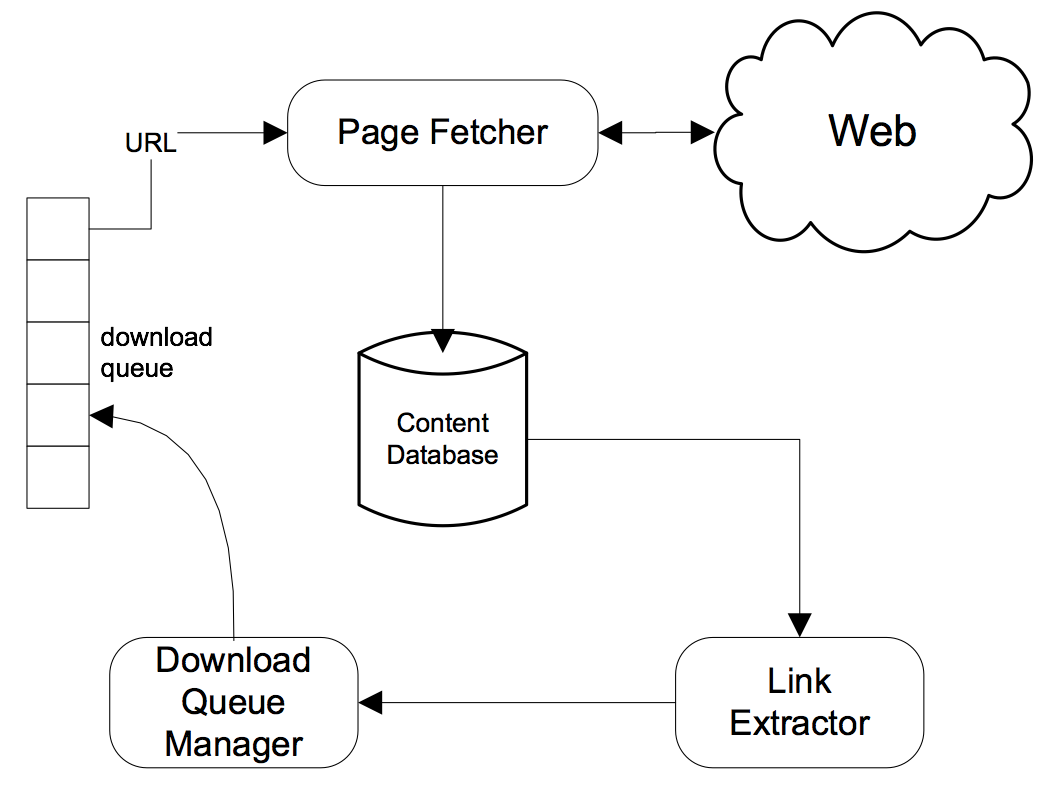
\includegraphics[scale=0.3]{Crawler_001}
		\caption{Basic web crawler algorithm.}\label{fig:Crawler_001}
	\end{figure}
		
	\begin{itemize}
		\item Content Selection: Crawlers should bypass irrelevant, low-quality, malicious content.
		\item Scale: Web hosts an enormous amount of data but the crawlers seek broad coverage and freshness.
		\item Speed: The basic and fast way of keeping track of visited URLs is storing in the memory. However, it is not possible to store hundreds of millions of URLs in the memory. That is why such lists are kept on disk, but accessing and re-ordering the list becomes slower and degrade the crawling performance.
		\item Infrastructure Cost: According to a blog post on the Official Google Blog \cite{A2013}, the Google index now contains about 1 trillion unique URL's. This graph of one trillion URLs is similar to a map made up of one trillion intersections, which is continuously reprocessed several times per day. Storing, indexing and fresh-keeping such a huge data requires massive investments on hardware infrastructure.
		\item Ethics / Politeness: Crawlers should prevent server overload and comply with Robot Exclusion Protocol according to Koster in his article \cite{K2013}: \emph{"A standard for robot exclusion."}(which is a de facto standard for definition of access rights on a website for crawling).
	\end{itemize}
	
	\subsubsection{Focused Web Crawling}\label{focusedWebCrawling}

	One of the most important properties of a crawler is the speed; this becomes even more important when we think about the web hosting an enormous amount of data in various forms, structures, formats, etc. Is estimated to have more than 10 billion pages and continues to grow rapidly according to the work of Kunder \cite{WWW2013}. 
	
	
	Crawlers should discover and use not only the new pages but also the recent versions of the pages. A general purpose crawler is said to be neither necessary nor sufficient to crawl and index such a giant amount of web pages. Therefore, a specialised version of crawling, called focused web crawling, is proposed aiming to collect on-topic data which actually reduces the search space.
	
	The first related work on focused crawling was done by De Bra in his article \emph{"Information retrieval in distributed hypertexts"} \cite%[p. 481-493]
	{B1994}, called fish search. In this research, for a client-based search engine, a simulated group of fish crawls on the web and assigns page relevance metric to pages using a binary classification with an input of simple keyword or regular expression. The lifespan of a fish depends on visited page relevance, where the fish dies when a specified amount of irrelevant pages are traversed. In addition, a fish produces offspring when a new page is traversed. Fish search works as depth-first search, since new URLs are added to the beginning of the download queue.
	
	Later, an extended version of fish search was developed, so called shark search, it was proposed by Hersovici in his article: \emph{"The shark-search algorithm"} \cite%[p. 317-326]
	{H1998}. In contrast to fish search, shark search estimates page relevance with a continuous function resulting a real number between 0 and 1 for the a similarity between document and query. Then, in the download queue, URLs are ordered by linear combination of source page relevance, anchor text and neighbourhood of the link on the source page.

	\subsection{Sentiment Analysis}
	
	Opinions as the key influencers of our behaviour are important. As Liu \cite%[p. 459-460]
	{L2011} stated, our beliefs and perceptions of the reality, and the choices we make, are susceptible on how others see and evaluate the world. This is the reason why people seek out opinions of others when making a decision. Sentiment analysis (a.k.a. opinion mining) is an area of study and analysing people's opinions, appraisals, attitudes, feelings, and emotions toward entities, individuals, issues, events, topics and their attributes. Sentiment analysis has been an active research area for quite some time. Feldman \cite%[p. 82-89]
	{F2013} states that there are over 7,000 articles on the topic of sentiment analysis, and apart from the techniques applied, all sentiment analysis systems implement a generic pipeline, which is illustrated in Figure \ref{fig:Sentiment_001}.
	
	\begin{figure}\centering
		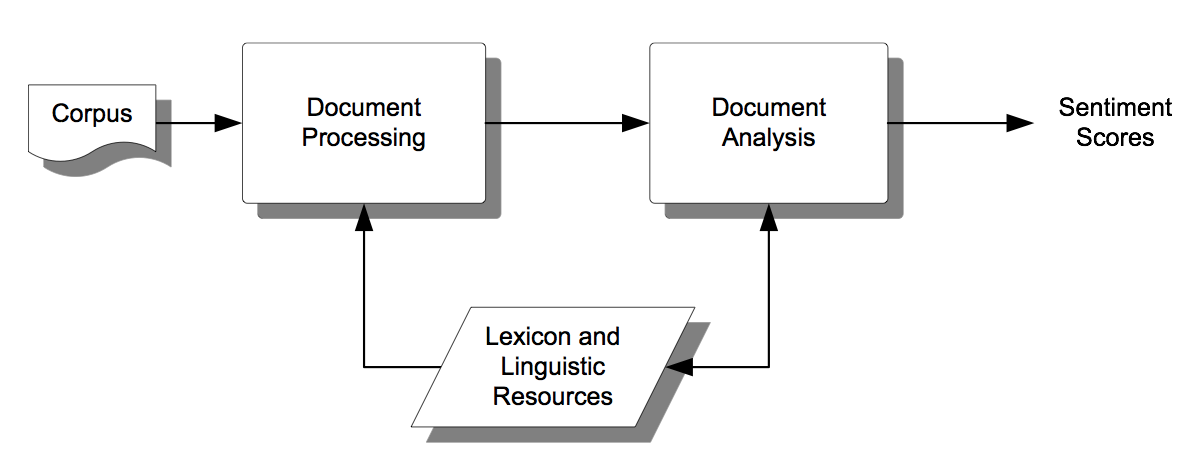
\includegraphics[scale=0.3]{Sentiment_001}
		\caption{The pipeline of modules in a generic sentiment analysis framework.}\label{fig:Sentiment_001}
	\end{figure}
	
	The input for a sentiment analysis framework is a corpus of documents, which may include a web page, news articles (which is particularly our case), a short post or a text document in any format. The corpus is pre-processed by document processing module, which converts corpus to texts by using linguistic resources for stemming, tokenization etc. Then pre-processed texts are sent to the document analysis module which annotates them using the linguistic resources and sometimes with a dictionary of words, called lexicon, which includes annotations of word's sentiment strength. The primary source of subjective content in a textual content can be adjectives (\cite{H1997}, \cite{H2004}), adverbs \cite{B2007}, adjectives and verbs \cite{K2004} or exclusive use of verbs \cite{S2008}. The output of the framework is the annotations which can be attached to whole document, to sentences, to entities as sentiment scores.
	
	The document analysis module, which is the main module of the framework, can apply two main lines of techniques for annotation: machine-learned and lexicon-based. In machine-learned sentiment analysis techniques \cite{P2002}, a model is built by a training dataset using common machine learning algorithms such as SVM, Naive Bayes, Logistics Regression, or KNN. Each document instance (e.g., a product review) in the dataset is associated with a value indicating the strength and polarity of the sentiments expressed in the text. In practice, obtaining large-scale labeled datasets is difficult, and the existing datasets are often domain-specific. As a remedy, the lexicon-based sentiment analysis techniques (\cite{B2010}, \cite{T2010}, \cite{TB2011}) aim to create a vocabulary and a set of rules to quantify the amount of sentiments in a given piece of text, eliminating the dependency to labeled training data. The vocabulary and rules are created manually, or by utilising resources like WordNet \cite{M1995}.
	
		
	\section{Structure of the work.}

	\begin{itemize}
		\item \textbf{Chapter \ref{introduction}} introduces the thesis, its goals and the current state of the art of \emph{Web Crawlers} and \emph{sentiment analysis}.
		\item \textbf{Chapter \ref{backgroundRelated}} presents the theoretical background needed in order to develop the technical and practical parts of the thesis. Besides in this chapter is presented the related work previously done in the field of news article analysis and its application to the stock markets.
		\item \textbf{Chapter \ref{analysisDesign}} introduces the analysis and design of the framework, this chapter is segmented in the design and analysis of the two main components: the \emph{news crawler} and the \emph{sentiment analysis}.
		\item \textbf{Chapter \ref{Realisation}} describe in detail how the framework was implemented, how to configure it, class diagram, data model and libraries used.
		\item \textbf{Chapter \ref{experimentalEvaluation}} shows experimentally how the multi-threading improved the performance of the framework, its thresholds with the available hardware. Besides we will make a simple analysis on the obtained data for \emph{the current most valuable company in history (so far)} \cite{BE2012}.
	\end{itemize}
	
	
.
	
	
	
	
	
	
	
		




		
	\setsecnumdepth{all}
	
	\chapter{Theoretical Background and related work}\label{backgroundRelated}
	
		Due to the technical nature of the work, there are until these days only few authors that refers to this topic, mostly in papers or articles, or journals; in which they don't provide that much technical information.\\
Anyways, we will mention here the most important details about some related work that have been done that can help us in the development of this work.\\\\
First we will start with the work of Robert Schumaker \cite{SCH2012}, \cite{SCH2010}, \cite{SCH2010-1}. He is an Associate Professor of Management Information Systems at Central Connecticut State University. We will dig into each of this papers that are previously cited.\\ We will start with the paper named: "Sentiment Analysis of Financial News Articles" \cite{SCH2012}. In this paper, the author mentions that the prediction of the stock price has always had certain appeal to researchers, and then it came the one biggest questions in stock markets:  \emph{Does price history matter?}. According to the author, new information is introduced to the market all the time, while a variety of information sources can all move a stock price, e.g., rumors, eavesdropping and scandals. Financial news articles are considered more stable and a more trustworthy source. We will quote some textual words from the author.\\

\emph{"However, the exact relationship between financial news articles and stock price movement is complex. Even when the information contained in financial news articles can have a visible impact on a security’s price [Gidofalvi 2001 \cite{GG2001}; Lavrenko, Schmill, Lawrie, Ogilvie, Jensen \& Allan 2000a \cite{LSL2001}; Mittermayer 2004 \cite{MM2004}; Wuthrich, Cho, Leung, Permunetilleke, Sankaran, Zhang \& Lam 1998 \cite{WC1998}], sudden price movements can still occur from other sources, such as large unexpected trades [Camerer \& Weigelt 1991 \cite{CW1991}]."}\\

This previous works, rely on financial documents from reputable Web sources, there are many financial news aggregation sites to provide this service. One of these sites is Comtex, which offers real-time financial news in a subscription format. Another source is PRNewsWire, which offers free real- time and subscription-based services. Yahoo! Finance is a third such source and is a compilation of 45 different news sources including the Associated Press, Financial Times and PRNewsWire among others. This source provides a variety of perspectives and timely news stories regarding financial markets.

In our case, we will rely on one "reputable" source that the only thing it does is to collect news from around 800 different sources. In this case we are talking about \emph{Google News}.

		
		\clearpage
\section{Theoretical Background}

Before we will go deep, we will establish a theoretical background to clarify some concepts that we will be using on this work. 

\subsection{Finances}

First, we will start with some non-computer-science related topic, that in our case is important because we need to understand the basics of \emph{why stock prices change?}, and for this we will rely on the work of Pattel: \emph{"Profit from prices"} \cite{P2007}.


 \subsubsection{How the market works?}
	\emph{"Any market is made of buyers and sellers/suppliers and there is always a conflict going on between these two groups. Buyers want to pay the minimum possible price while sellers on the other hand want to get maximum possible price. If the price is too low, buyers would demand a large quantity but sellers would not want to sell much at this low price. If price is too high, sellers would love to sell a large quantity but buyers would not want to buy much. This is a kind of war between two groups - one trying to push prices lower and the other one trying to push prices higher. In market economy, price keeps changing until it reaches a point where the quantity demanded by buyers equals quantity supplied by sellers."}

 \subsubsection{What causes stock prices to change?}
	\emph{"One will see these Demand and Supply curves change more rapidly for a stock than for any other item. That is why we see stock prices changing almost every moment. For a stock, individuals and institutions that hold the stock or intend to short the stock are the potential sellers and they collectively define the supply curve. There are thousands, if not millions, of reasons that may motivate or prompt a market participant to sell a particular stock he or she is holding or intending to short sell. Similarly, individuals and institutions that are thinking/planning to buy the stock form the Demand curve. There would also be several reasons why they want to buy this stock. As we all know, a stock’s price is likely to go up if the Demand is increasing or the Supply is decreasing. Similarly it is no rocket science to figure out that a stock’s price would drop if the Demand is shrinking and/or the Supply is expanding. So when a trader is buying a stock, he wants its prices to go up after he has bought it. He wants the Demand for the stock to go up or the supply to dry up."}
	
 \subsubsection{How often the stock prices change?}
	\emph{"The demand and supply curves for any stock are constantly changing. Variety of economy, industry related or company related events, news, discussions, analyst reports and political and global developments constantly change the demand and supply curves for any stock. Add to this, the fact that given a certain piece of information, a person can’t be sure how people will react to it. Aren’t you surprised to see that even after some unexpected strong positive news about a stock, the stock keeps being traded! Ideally, if the news is too good, everybody should be a buyer and there should be no seller! If there were no seller, there would be no trade! But the fact that most of the stocks keep trading every moment when the Market is open indicates just one thing: There are people with totally different views about the prospects of a stock at any given moment. Everyone who is driven to buy or sell a stock has his own criteria to value the stock, his own set of expectations, and his own unique financial situations and circumstances. This makes it almost impossible to draw complete demand and supply curve for any stock at any point in time."}
	
 \subsubsection{What does the stock price represent?}
	\\ \emph{"The net impact of everything happening in a stock or a company gets immediately reflected in the price of the stock. Price is the point where millions of different counter acting forces balance out. So with enough attention to changes in the price of a stock over a day or two, there will be times when we can visualize changes that are taking place in aggregate demand/supply of that stock, and based on that, we will be able to determine in which direction the price of the stock is likely to move over the next few days. There is no need to get into complex world of demand and supply curves; all we need is to keep an eye on where the balance between them is heading."}


\clearpage
\subsection{Parallel Computing}\label{ParallelComputing}

In order to evaluate our gain or loss by implementing multi-threading in our framework we will cite the work of Professor Tvrdík \cite{T2011} in the chapter of his book \emph{Performance and Scalability of parallel algorithms}, where there are some useful metrics to measure the performance of parallel algorithms. We will be using this metrics further in our work.


 \subsubsection{Parallel time T(n,p)}\label{ParTime}
Is the time elapsed from the beginning of a p-processor (In our case we will consider software threads) parallel algorithm solving a problem instance of size \emph{n} until the last processor finishes the execution. \emph{T(n,p)} is obtained by \emph{counting} or by \emph{measuring the total time complexity} of:
	\begin{itemize}
		\item \emph{parallel computationl} steps. e.g., arithmetic operations.
		\item \emph{parallel communication} steps. i.e., transfers and exchanges of data between processors.
	\end{itemize}	
	Due to the second component \emph{T(n,p)} depends on the architecture of a parallel computer. Therefore the performance evaluation of a parallel algorithm must \emph{always} consider the architecture. In a specific algorithm, \emph{p} is always chosen as a suitable function of \emph{n}.

 \subsubsection{Parallel Speedup S(n,p)}\label{ParSpeedup}
If both, sequential and parallel algorithm with \emph{p} processors are executed under the same conditions, the best speedup we can hope is for \emph{p}. Due to the communication overhead, such a speedup is achievable only if the solution of the problem contains enough parallelism, the communication part is negligible, and all the processors perform only useful computation under ideal load balancing and synchronisation. In practice, a linear speedup \emph{k*p} for some constant 0 \textless k \textless 1 is quite satisfactory.
	
 \subsubsection{Parallel cost C(n,p)}\label{ParCost}
	\[C(n,p) = p * T(n,p) \] 
	This metric is a bit coarse-grained. It is actually an upper estimate of the operational complexity. It gives the total number of operations as if all processors were active since the beginning till the end (like the slowest processor). But this is what parallel systems with job schedulers typically allow: prior to a parallel computation, a user job is assigned p processors and these are released only after the whole parallel computation has finished. In such systems, \emph{C(n,p)} is a useful metric, since idling processors or processors that finished their subtasks faster are useless for the other users until the whole computation finishes. Since any parallel algorithm can be trivially simulated on a uniprocessor machine with multiprogramming, we get that \emph{The parallel Cost, cannot be less than the complexity of the best sequential algorithm:}
	\[C(n,p) = \Omega(SU(n)) \] 
	\emph{In the best case, the cost is of the same order as the sequential complexity:}
	\[C(n,p) = O(SU(n)) \] 
	
 \subsubsection{Parallel Efficiency E(n,p)}\label{ParEfficiency}
	\[E(n,p) = \frac{SU(n)}{C(n,p)} = \frac{S(n,p) * T(n,p)}{p * T(n,p)} =  \frac{S(n,p)}{p} \leq 1 \] 
	Basically, the Parallel efficiency is the speedup per processor.

 \subsubsection{Barrier Synchronization}\label{BarrierSynchronization}
	Each processor stops at a logical point in the program until all processor arrives to this point. Then all processors can continue.

\clearpage
\subsection{Statistics}\label{statistics}

In our work, there are several statistics-related topics, which we need to understand and clarify, because our \emph{Sentiment Analysis Framework} (\ref{sentimentAnalysis}) rely mostly on \emph{Pointwise mutual information - PMI} (\ref{PMI}). We will need as well another simple concept for the analysis that we will be performing to the retrieved information in chapter \ref{experimentalEvaluation}, which is the \emph{Pearson correlation coefficient} (\ref{PearsonCorr}).

\subsubsection{Random Variables}\label{RandomVariable}

In order to define our framework, first we need a simple statistical concept and we will rely on the work of Anderson \cite{AN2011}; A \emph{Random variable} is a numerical description of the outcome of an experiment, and its particular value depends on the outcome of the experiment, and they can be classified as being either \emph{discrete} or \emph{continuous} depending on the numerical value it assumes.

In our case, for this work , we will focus on the \emph{discrete} random variables, which assume either a finite number of values or an infinite sequence of values such as 0,1,2, ..., +\infty.

We will use the \emph{Discreate random variables} when we will calculate the \emph{Pointwise mutual information} (\ref{PMI}).

 \subsubsection{Mean}\label{mean}

This is quite common, simple and useful concept. In order to establish the mathematical background, we will define the \emph{Simple arithmetic mean} relying on the work of Arulmozhi \cite{ARU2009}, which is obtained by summing up all elements \begin{math}X_{i}\end{math} of the set and divide it by the number of computed elements. Mathematically is defined as follows:

\begin{equation} \label{eq:Mean}
	\bar{X} = \frac{1}{n} \sum ^n _{i=1}X_i
\end{equation}

\subsubsection{Variance}\label{variance}

In order to introduce the \emph{Pearson correlation coefficient} (\ref{PearsonCorr}), we first must define how it is composed, for that we will start with the \emph{variance}, and we will rely on the work of Anderson \cite{AN2011} which states that the \emph{variance} is a measure of variability that utilises all the data, and is based on the difference of the value of each observation \begin{math}X_{i}\end{math} and the mean. The difference between each \begin{math}X_{i}\end{math} and the mean (\begin{math}\bar{X}\end{math} for a sample, \begin{math}\mu\end{math} for a population) is called \emph{deviation about the mean}. For example, a deviation about the mean is written \begin{math}(X_{i} - \bar{X})\end{math}; for a population it is written \begin{math}(X_{i} - \mu)\end{math}. In the computation of the \emph{variance}, the deviations about the mean are \emph{squared}. 

If the data are for a population, the average of the squared deviations is called: \emph{the population variance}, which is represented by \begin{math}\sigma ^2 _{X_i}\end{math}.

In our case, we will use notation for the deviation about the mean \begin{math}(X_{i} - \bar{X})\end{math}, because we will be analysing a subset of the \emph{population} of news articles. We will exemplify for two \emph{random variables} it's variance in the equations: \ref{eq:VarX} and \ref{eq:VarY}, the Standard deviation is the square root of the variance of the random variable and is exemplified in the equations \ref{eq:sdX} and \ref{eq:sdY}.


\begin{equation} \label{eq:VarX}
	var X = \frac{\sum ^n _{i=1}{(X_i - \bar{X})}^2}{n}
\end{equation}

\begin{equation} \label{eq:sdX}
	Standard Deviation X = \sqrt{var X} = \sqrt{\frac{\sum ^n _{i=1}{(X_i - \bar{X})}^2}{n}}
\end{equation}

\begin{equation} \label{eq:VarY}
	var Y = \frac{\sum ^n _{i=1}{(Y_i - \bar{Y})}^2}{n}
\end{equation}

\begin{equation} \label{eq:sdY}
	Standard Deviation Y = \sqrt{var Y} = \sqrt{\frac{\sum ^n _{i=1}{(Y_i - \bar{Y})}^2}{n}}
\end{equation}


 \subsubsection{Covariance}\label{covariance}

Before introducing the \emph{Pearson correlation coefficient} (\ref{PearsonCorr}) we still need another statistical concept; \emph{covariance} which is a descriptive measure of the linear association or degree of overlap of the variables between two variables, it describes the extent to which a change in one variable (X) is paired with a comparable change in another variable (Y). For a sample size \emph{n} \begin{math}(X_{1},Y_{1}), (X_{2},Y_{2}), (X_{3},Y_{3}), ... , (X_{n},Y_{n}) \end{math} the sample covariance is defined according to Sharma \cite{PP2014} and Arulmozhi \cite{ARU2009} we have:

\begin{equation} \label{eq:PearsonCovariance1}
	Covariance (X, Y) = \frac{1}{n} \sum ^n _{i=1}(X_i - \bar{X})(Y_i - \bar{Y})
\end{equation}

According to the formula, is defined as the sum of the product of the deviations of the X and Y values from the means of X and Y.

 \subsubsection{Pearson correlation coefficient}\label{PearsonCorr}
 \emph{Pearson correlation coefficient} (Pearson's r) is a measure of the \emph{linear correlation} (dependence) between two variables X and Y, giving a value between \begin{math}+1\end{math} and \begin{math}-1\end{math} inclusive; as shown in the equation \ref{eq:PearsonRange}, where \begin{math}+1\end{math} is total positive correlation, \begin{math}0\end{math}is no correlation, and \begin{math}-1\end{math} is total negative correlation. It is widely used in the sciences as a measure of the degree of linear dependence between two variables.

Pearson's correlation coefficient between two variables is defined as the covariance (equation: \ref{eq:PearsonCovariance1}) of the two variables divided by the product of their standard deviations. The form of the definition involves a "product moment", that is, the mean (the first moment about the origin) of the product of the mean-adjusted random variables; hence the modifier product-moment in the name.

Pearson's correlation coefficient when applied to a sample is commonly represented by the letter r and may be referred to as the sample correlation coefficient or the sample Pearson correlation coefficient. And is calculated as follows: 

\begin{equation} \label{eq:PearsonExtended}
	r_{x,y} = \frac{\sum ^n _{i=1}(X_i - \bar{X})(Y_i - \bar{Y})}{\sqrt{\sum ^n _{i=1}(X_i - \bar{X})^2} \sqrt{\sum ^n _{i=1}(Y_i - \bar{Y})^2}}
\end{equation}

Simplifying the formula we will have:

\begin{equation} \label{eq:Pearson1}
	r_{x,y} = \frac{Covariance (X, Y)}{\sqrt{var X} \sqrt{var Y}}
\end{equation}

The range of the \emph{Pearson correlation coefficient}

\begin{equation} \label{eq:PearsonRange}
	-1 \leq r_{x,y} \leq +1
\end{equation}



We will mention some properties of the Pearson's coefficient according to Arulmozhi \cite{ARU2009}:

	\begin{itemize}
		\item The value of \begin{math}r_{x,y}\end{math} does not depend upon the units of measurement.
		\item The value of \begin{math}r_{x,y}\end{math} does not depend upon which variable is labeled X and which is labeled Y (\begin{math}r_{x,y} = r_{x,y}\end{math})
		\item Correlations lies between \begin{math}-1\end{math} and \begin{math}+1\end{math} as mentioned in the equation \ref{eq:PearsonRange}.
		\item If \begin{math}r_{x,y} = \pm 1\end{math} then all the points of the scatter diagram lie exactly on a straight line and the correlation is said to be positive perfect or negative perfect, depending on the sign of the correlation.
		\item \begin{math}r_{x,y}\end{math} measures only the linear relationship between X and Y.
	\end{itemize}



We will define some facts of the strength of the correlation.

	\begin{itemize}
		\item Strong or high correlation exists between between variables if  \begin{math}| r_{x,y} | \geq 0.75\end{math}
		\item Moderate correlation exists between the variables if \begin{math} 0.5 \leq | r_{x,y} | \leq 0.75\end{math}
		\item Weak or low correlation exists between the variables if \begin{math}| r_{x,y} | \leq 0.3\end{math}
	\end{itemize}


\subsubsection{Pointwise mutual information - PMI}\label{PMI}

In order to introduce the concept of \emph{Pointwise mutual information} we will rely on several authors. According to Gelbukh \cite{G2009} \emph{Pointwise mutual information} gives the direction and strength of association (whether a bigram occurs more often or less often than expected, based on the frequency of its parts), but this measure is unreliable with spare data.

Goldstein \cite{G2006} mentions that statisticians have devised methods for combining information in several conditional probabilities into a single number summarising the relevant information. One of this methods is \emph{Pointwise mutual information}, which is obtained by dividing the probability of two tonal sequences occurring together (in any order). Besides, is useful with binary events (e.g., boundary tones, which have only two values: H\% and L\%). When many tonal sequences are being considered, \emph{Pointwise mutual information} may produce a large array of numbers. To find a single number, one uses \emph{mutual information}, a weighted average of \emph{Pointwise mutual information} for every possible combination of tonal sequences. The weights used in the weighted average are given by the probability of each combination of sequences occurring.

All this concepts are useful for us, but we will try to keep it simple, and for this we will help ourselves with the work of Sundaram \cite{SD2006} which states that the mutual information between two variables is defined as \emph{Pointwise mutual information}. Mathematically is defined as follows: 

\begin{equation} \label{eq:PMI1}
\operatorname{pmi}(x;y) \equiv \log_{2}\frac{p(x,y)}{p(x)p(y)} = \log_{2}\frac{p(x|y)}{p(x)} = \log_{2}\frac{p(y|x)}{p(y)}.
\end{equation}

According to the equation \ref{eq:PMI1} \emph{x} and \emph{y} are two discrete and independent random variables, and they can be regarded as the amount of information \emph{x} contains about \emph{y}, and the quantification of the discrepancy between the probability of their coincidence given their joint and individual distributions.

And in our particular case and for our work, and as described by Trnka \cite{TR2011} we will approach the \emph{PMI} as the measure of how much one word tell us about the other, how much information we gain. This number can be positive or negative, as described in the equation \ref{eq:PMIRange}. For us, \emph{x} and \emph{y} are occurrences of particular words. The denominator \emph{P(x) * P(y)} is the expected value of \emph{P(x , y)}, assuming x and y are independent. 

\begin{equation} \label{eq:PMIRange}
	-\infty \leq \operatorname{pmi}(x;y) \leq +\infty
\end{equation}
	
	\chapter{Analysis and design of the framework}\label{analysisDesign}
	
		%%%%%%%%%%%%%%%%%%%%%%%%%%%
%%%%%%%%%NEWS CRAWLER%%%%%%%%%
%%%%%%%%%%%%%%%%%%%%%%%%%%%
In this chapter we will analyse the two basic components of this work, and we will design a solution in which the output data of the first one (News Crawler \ref{newsCrawler}) will be the input data of the second one (Sentiment Analysis \ref{sentimentAnalysis}). For this we will introduce some simple and general sequential algorithm that will give us a brief overview of how we will deliver our solution.


\begin{algorithm}
\caption{General Algorithm}\label{generalAlgorithm}
\begin{algorithmic}[1]
\FOR {\text{each company}}
	\STATE \text{Crawl News articles;}
	\STATE \text{Extract} \textit{article: date, title, content, author}\text{;}
	\STATE \text{Classify} \textit{article}\text{;}
	\STATE \text{Save} \textit{article}\text{;}
\ENDFOR
\STATE \text{Summarize} \textit{articles}\text{;}
\STATE \text{Download \& Save} \textit{stock prices}\text{;}
\end{algorithmic}
\end{algorithm}

Each part of the algorithm \ref{generalAlgorithm} will take one or several sections in this work, besides is the highest level of abstraction of the tasks that will be performed. This process will be repeated for each of the previously defined companies (see the table \ref{tab:analyzedCompanies}). Basically, we will crawl the news for every company (as shown in section \ref{newsCrawler}) and we will extract the information of our interest (as described in section \ref{locators}), after this we will classify the article in positive or negative (according to the section \ref{sentimentAnalysis}), finally we will be saving every article in our page repository \ref{pageRepository}. When we will finish the iteration, for all companies we will summarise the data and download the stock prices as described in the section \ref{priceRetrieval}. Later, with this data we will perform a statistical analysis (Pearson correlation \ref{PearsonCorr}), based on the assumption that the data that we obtained share a \emph{linear relationship}.


\section{News crawler}\label{newsCrawler}

This section will describe how the task of "news article retrieval" was performed in order to get the right data from the news endpoint.
In a perfect world when every Web application/Web page has its own Web API the "article retrieval" would be a trivial task that would consist on consuming a Web API and we would get structured information, but unfortunately not all web pages allows access to their information through Web API.
We will use as news endpoint "google news"; even if it doesn't have a Web API, because the news articles there, are already categorised by company and date.

By crawling "google news", we will basically get links of articles pointing to different web pages; not articles \emph{per se}. This suppose a problem because every web page has different html structure. So, our crawler must be smart enough to associate one host to one particular page structure. To solve this problem we will introduce the term: Locators, which basically define for every host where is the data that we will extract.

To get this information, we will develop what is called in Liu \cite%[p. 312]
{L2011}: "A focused crawler" \ref{focusedWebCrawling}, where we will focus on \emph{news articles} of a particular company. Besides, we will make several modifications to this algorithm in order to adapt it to our needs. A basic focused web crawler is shown in the figure: \ref{fig:Crawler_002}, our classifier will be based on the fact that we only want news articles, and we will crawl our seed with different parameters (table \ref{tab:query-string}) in order to obtain the desired data.

	\begin{figure}\centering
		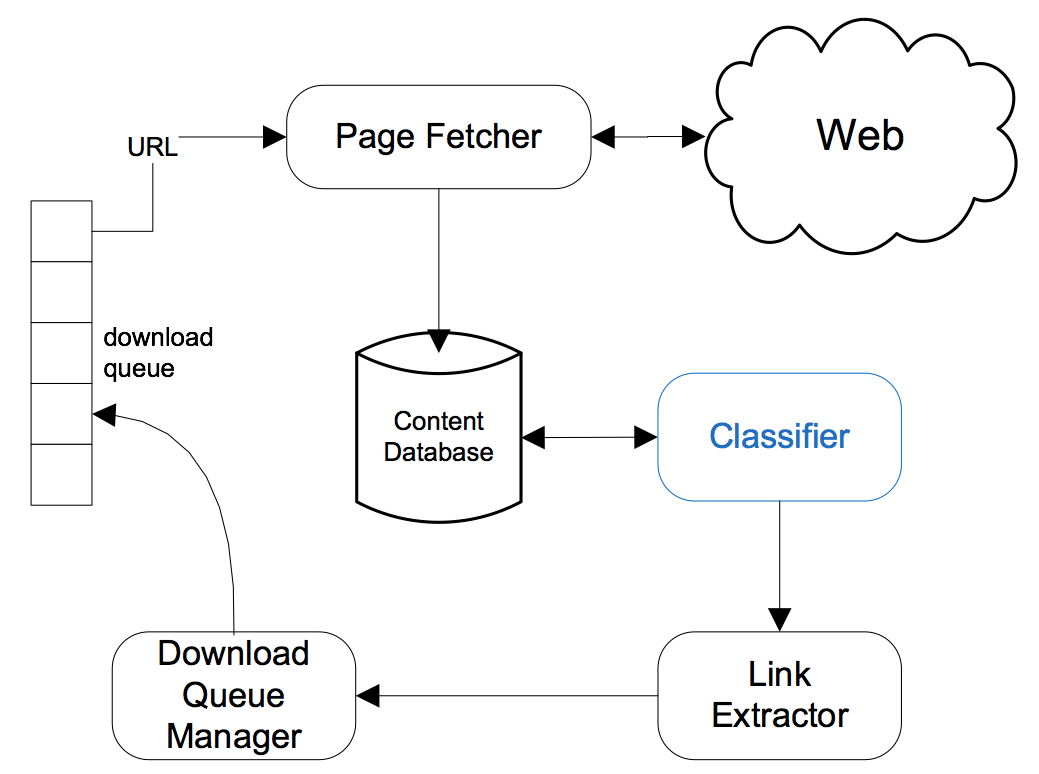
\includegraphics[scale=0.3]{Crawler_002}
		\caption{Basic focused web crawler algorithm.}\label{fig:Crawler_002}
	\end{figure}

\begin{algorithm}
\caption{Crawler Algorithm}\label{crawlerAlgorithm}
\begin{algorithmic}[1]
\STATE \text{Set } \textit{timeout;}
\STATE \text{Initialize } \textit{locators;}
\STATE \text{Initialize } \textit{seed(s);}
\STATE \text{Send } \textit{request;}
\STATE \text{Recieve } \textit{response;}
\STATE \text{Parse } \textit{response;}
\STATE \text{Extract } \textit{links} \text{ of our interest;} 
\FOR {\text{each} \textit{link} }
	\STATE \text{Save } \textit{link;}
	\STATE \text{Load } \textit{locator} \text{ for the host;}
	\STATE \text{Extract from} \textit{link: date, title, content, author}\text{;}
	\STATE \text{Save extracted data;}
\ENDFOR
\end{algorithmic}
\end{algorithm}

\subsection{Web Crawler}\label{webCrawler}

According to Liu \cite%[p. 311]
{L2011} a Web crawler is basically a program that automatically download Web pages. To build the Web crawler, we will need a set of seed pages; in our case, our main seed will look like follows: 
\\\\
\url{https://www.google.com/finance/company\_news?q=\%s&start=\%s&num=\%s}
\\\\

	\begin{figure}\centering
		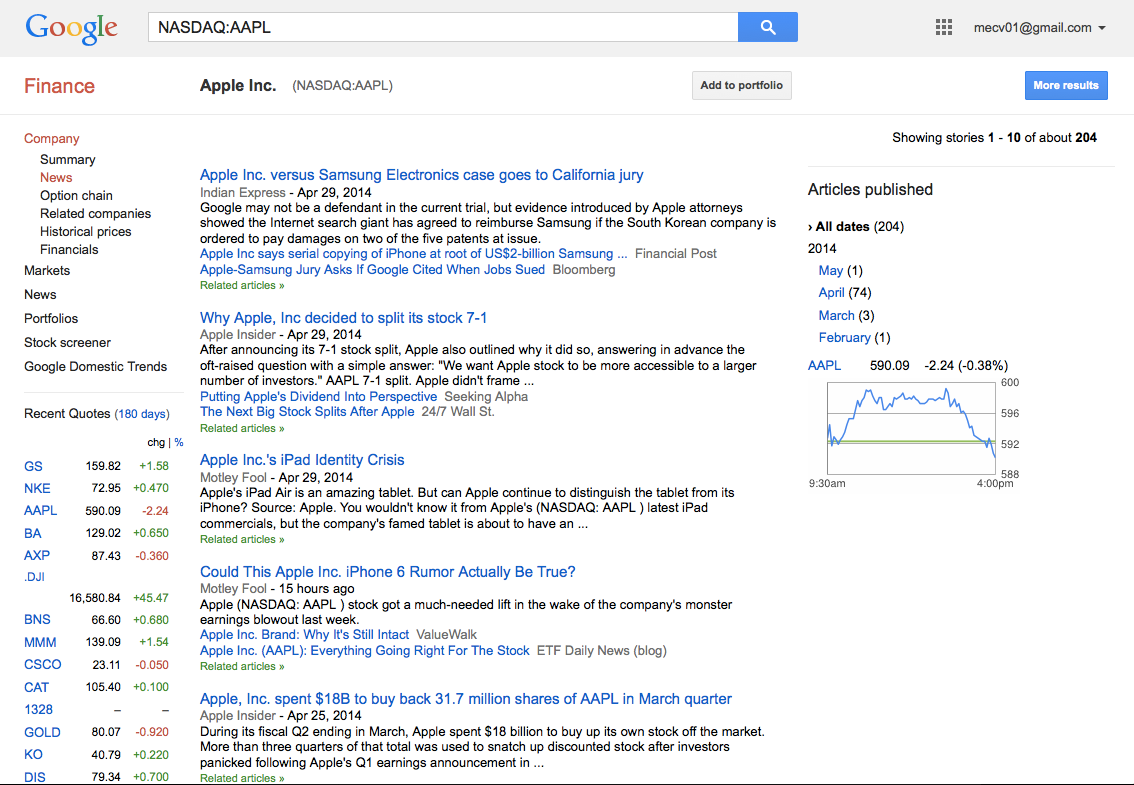
\includegraphics[scale=0.35]{News_001}
		\caption{Screenshot of Google News.}\label{fig:News_001}
	\end{figure}

Every variable in the query string will represent something in particular, as described in  the table \ref{tab:query-string}.

\begin{table}\centering
	\caption{Query string variables}\label{tab:query-string}
   	\begin{tabular}{ | l | p{4cm\textwidth} | p{6cm\textwidth} |}
   	\hline
   	\textbf{Variable}  & \textbf{Explanation} & \textbf{Example}  \\ \hline
    	q & 
	In this variable, we will put the code of a particular company in the stock market.  & 
	Supposing that we want to retrieve all the news of apple(AAPL), the we will send: q=AAPL\\ \hline
	start & 
	This variable define in which index we will start watching the news.  & 
	Assume there are 100 news available, and I want to start in news article number 20; so, we will send: start=20 \\ \hline
	num & 
	This variable define how many news articles I will retrieve in one request. Maximum per request is 50. &
	We could use the previous example, assume we are starting in news article number 20, and we want to see the next 10 articles; so, we will send: start=20 and num=10 \\ \hline
    \end{tabular}
\end{table}

For each company we will generate \textit{N} number of links depending to the number of published articles per company. In every link that we will generate and crawl, we will find news articles links which will be pendant to be visited, these links are called:  \textit{the frontier}; which for efficiency matters and because of its small size (up to 50 links per crawled seed) will be stored in the main memory.

At the end we will have some sort of "preferential crawler"  \cite%[p. 314]
{L2011} due to not all the links of the page will be interesting for us; only the article links. From here, we will extract the article link, date, and title. To get this data we must check deeply the structure of the web page, to figure it out we help ourselves with \emph{Firefox developer tools}, which is a plugin of the Firefox Web browser, it will allow us to know the location (that's why further we will call this part of the application \emph{Locators}) of the element (title, date, link) of our interest. We can see in the figure \ref{fig:News_002} the plugin where we locate the main container of one particular news article. After identifying the container of the news article, we must identify the location of the title of the article, which contain as well the link of the article as shown in the figure \ref{fig:News_003}, and the last part would be to identify the date of the article, as shown in the figure \ref{fig:News_004}. 

	\begin{figure}\centering
		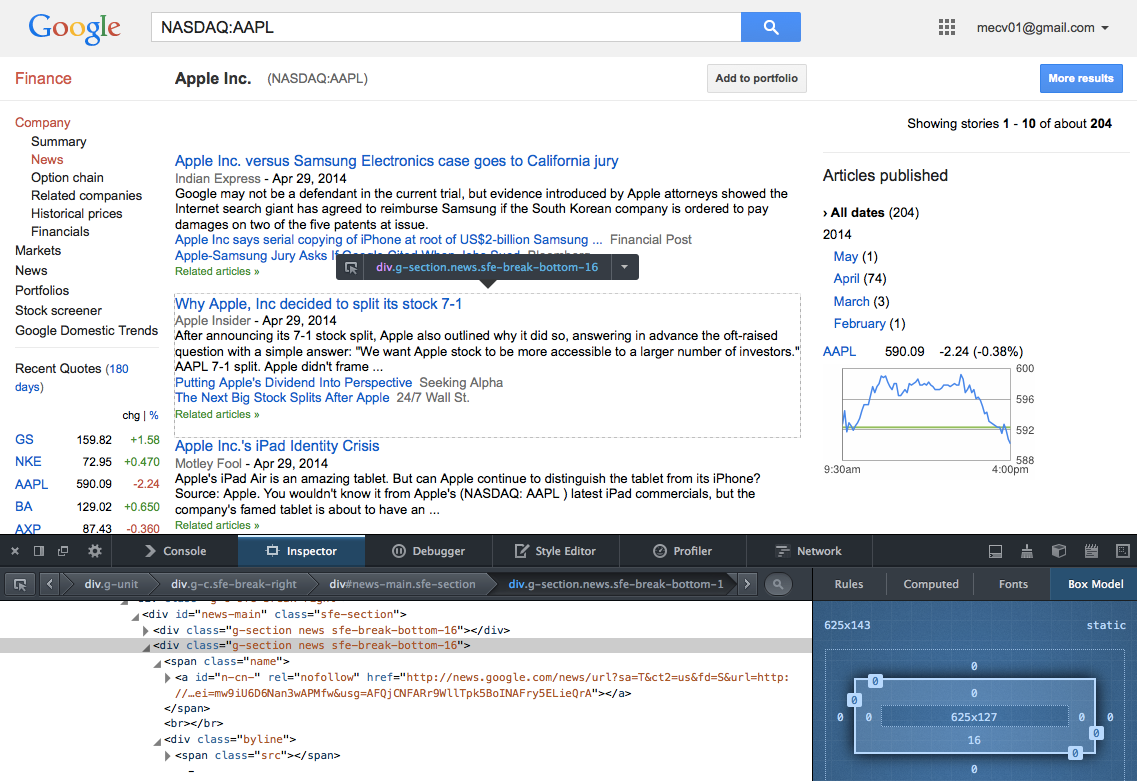
\includegraphics[scale=0.35]{News_002}
		\caption{Container of every article.}\label{fig:News_002}
	\end{figure}
	
	\begin{figure}\centering
		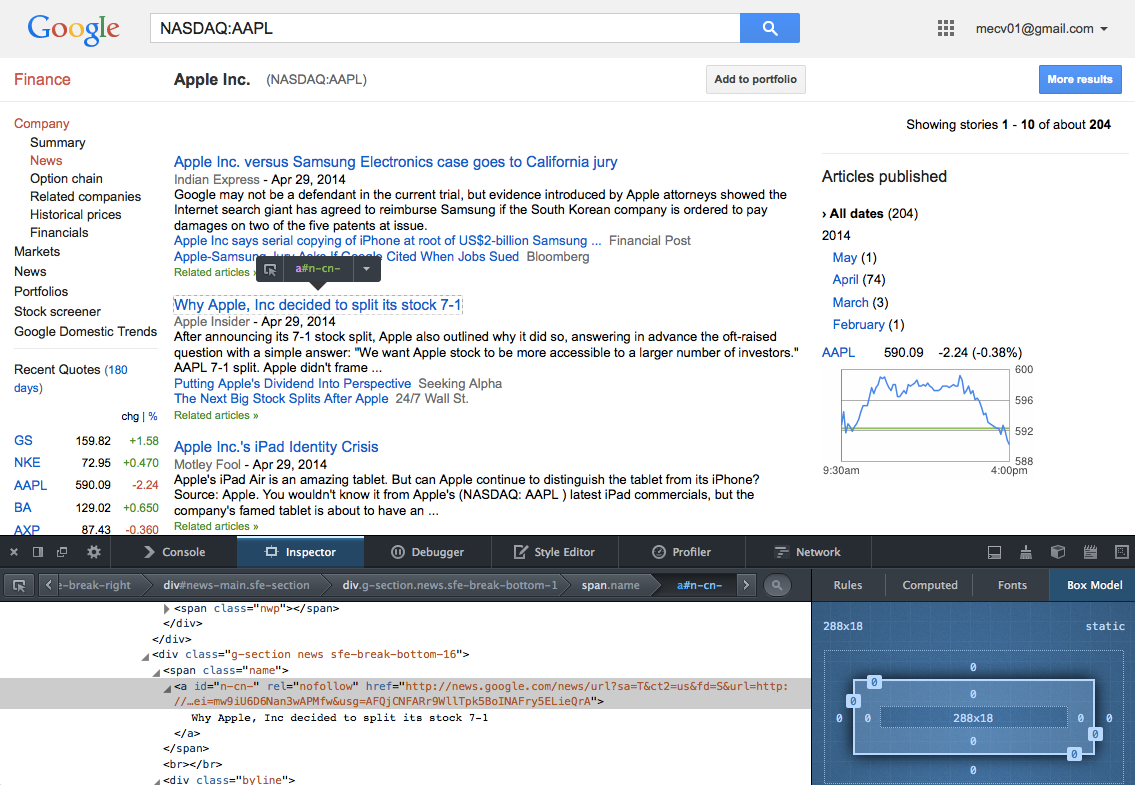
\includegraphics[scale=0.35]{News_003}
		\caption{Title of the article.}\label{fig:News_003}
	\end{figure}
	
	\begin{figure}\centering
		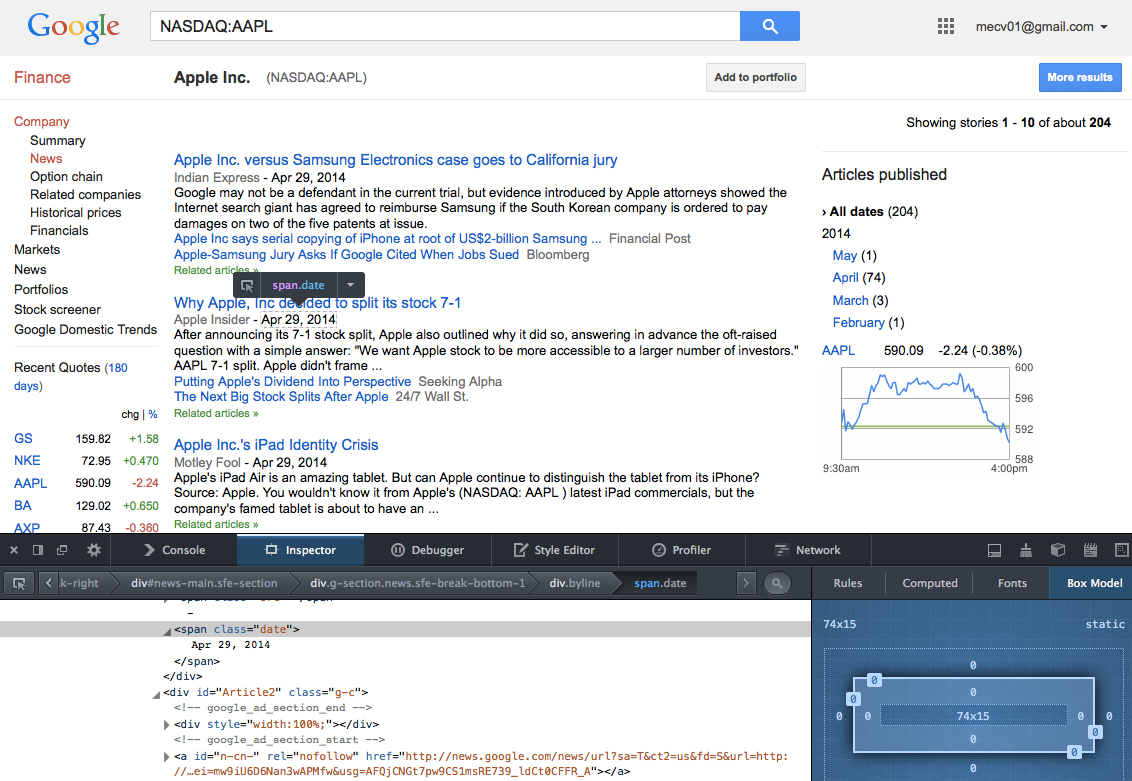
\includegraphics[scale=0.35]{News_004}
		\caption{Date of the article.}\label{fig:News_004}
	\end{figure}

\subsection{Implementation Issues}\label{implementationIssues}
In this section we will describe the "Implementation Issues" that we faced.
%\cite[p. 315]{L2011}
We will use one open-source tool: "jsoup" in order to download and parse a web page, so we will abstract this part, and we will focus on our main aim: news articles.

\subsubsection{Fetching}\label{fetching}
Once we have a particular link, and we will proceed to download the Web page, one important detail must be taken in consideration: \textit{timeout} connections; in the case of the application this parameter will be set to 30 seconds; which of course can be changed in the configuration file that we will call: "jsoup.properties". This part will be delegated to jsoup.

\subsubsection{Parsing}\label{parsing}
Again, the parsing part will be delegated to jsoup. Which manages in a good and efficient way the whole page structure by using "hash tables." In our particular case, once we fetched and parsed the article web page, we need to extract only the data that we are interested in. For this, and as we mentioned at the beginning of this chapter , we will introduce the term: "Locators" in the next section.

\subsubsection{Locators}\label{locators}
The aim of the "news crawler" is basically to extract \textit{title, date, author, content} from a particular article, and if we take in consideration that every Web page has \emph{different structure}, we need to define an extra component in order to extract accurately the information that we needed. We must mention that this method is very accurate when it tries to retrieve the article data.

We will define a Locator as a custom data structure that holds the particular representation of the structure of a web page in a particular host, in order to retrieve the data that we want. For this purpose a class can be found under the package: "com.carramil.dp.crawler" called: "Locator.java", and this class has its input data in a properties file which we called: "crawler.properties". The structure of this file is as follows: We will enumerate \textit{N} number of hosts from 1 to \textit{N} and for each of them we will define the required information as shown in the table: \ref{tab:locator}. Each item between semi-colons is a path to a particular tag; if we want to specify a path we must do it by separating every tag with "-$>$". It is important to mention that there must not be blank spaces between each semi-colon (";"), and in the case one particular host has several different page structures we can use ampersand ("\&") to separate between tags. We will mention an example in order for this part to be clear.

\begin{table}\centering
	\caption{Locator format}\label{tab:locator}
   	\begin{tabular}{p{11.5cm}}
   	\hline
GenericCrawler.source.1 = host;title;content;author;date;dateFormat\\
GenericCrawler.source.2 =host;title;content;author;date;dateFormat\\
GenericCrawler.source.3 =host;title;content;author;date;dateFormat\\
... up to \textit{N} ...\\
GenericCrawler.source.\textit{N} =host;title;content;author;date;dateFormat\\
    \hline
    \end{tabular}
\end{table}

\begin{table}\centering
	\caption{Locator example}\label{tab:locatorExample1}
   	\begin{tabular}{p{11.5cm}}
\lstset{language=HTML}
\begin{lstlisting}
<!DOCTYPE html>
<html>
<head>
    <title>my Page title</title>
</head>
<body>
	<div id="menu">
		The menu of the Web Page
	</div>
	<div class="meta-data">
		<h1>Title of the article</h1>
		<div class="author">
			By: <a href="#">Author Name of this article</a>
		</div>
		<div class="dateTime myFormat">
			Oct 9, 1985
		</div>
	<div >
	<div id="articleBody">
		This will be the body of the article
	</div>
</div> 
</body>
</html>
\end{lstlisting}
    \end{tabular}
\end{table}

In this example listed in the table: \ref{tab:locatorExample1} we will identify each of the things that we will be interested in, we will start with title: "body-$>$div.meta-data-$>$h1" and the result according to the example would be "Title of the article", we could define the locator by just specifying the tag "h1", because in this case the tag is unique in the document.

To get the content of the article we can construct the following locator: "body-$>$div\#articleBody" or as mentioned before "div\#articleBody" works for our purposes.

To get the date of the article the locator follows the pattern: "body-$>$div.meta-data-$>$div.dateTime.myFormat", and we have to specify to the Locator the format of this date; in this case is: MMM dd, yyyy. Remember that we can specify more than one date format.

The author would be retrieved as follows: "body-$>$div.meta-data-$>$div.author-$>$a".

Once we have this information from a particular host, the complete locator would be:\\
\emph{
GenericCrawler.source.1 = "www.host.com;body-$>$div.meta-data-$>$h1;\\
body-$>$div\#articleBody;body-$>$div.meta-data-$>$div.author-$>$a;\\
body-$>$div.meta-data-$>$div.dateTime.myFormat;MMM dd, yyyy"
}
\\\\
An actual example of a Locator:

\emph{
"GenericCrawler.source.2 = www.reuters.com;h1;\\
span\#articleText\&div.columnLeft-$>$p;p.byline;span.timestamp;\\
EEE MMM dd, yyyy hh:mma z\&dd MMM yyyy\&\\
MMM dd, yyyy\&EEE, dd MMM yyyy\&EEEE, MMM dd yyyy"}

But how to create a locator? we make a reference to \ref{crawlerProperties} in order to make an example on how to create one locator. And we will recall the \emph{Locator} of one particular how: \url{http://www.fool.com}, and we will use the following article to state the example:\\\ \url{Fool.com/investing/general/2014/04/29/apple-incs-ipad-identity-crisis.aspx}

\begin{itemize}
	\item First of all, we will consider the previously mentioned url, it looks like in figure \ref{fig:Locator_001}.
	
\begin{figure}\centering
	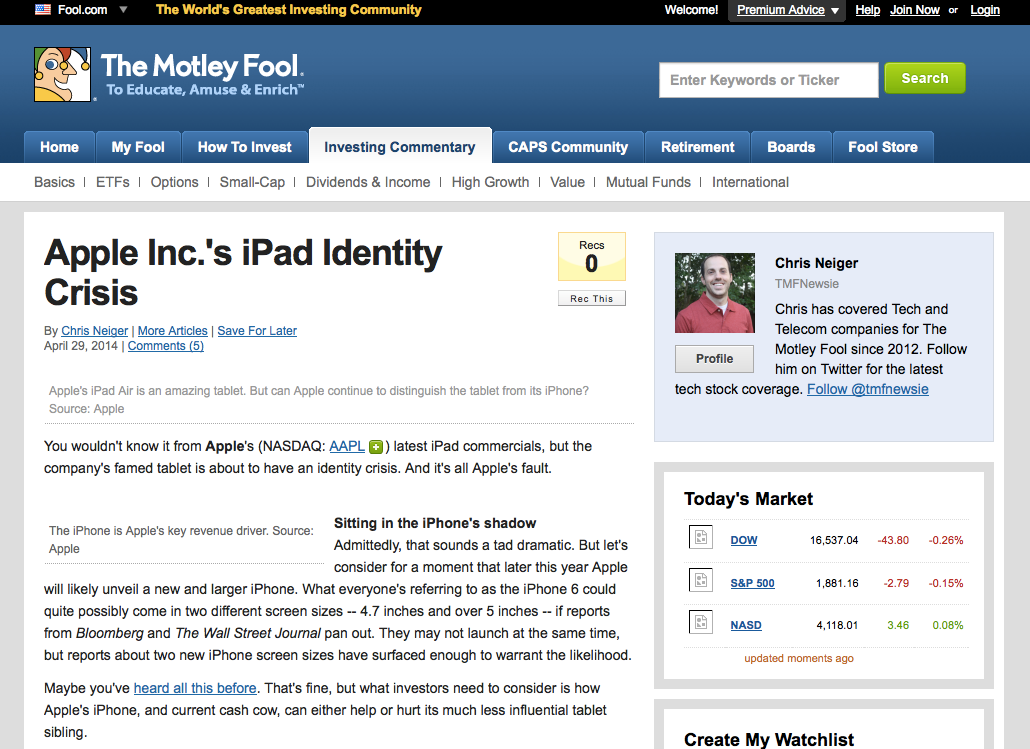
\includegraphics[scale=0.4]{Locator_001}
	\caption{Initial Web page.}\label{fig:Locator_001}
\end{figure}
	
	\item Then we must identify where is the location of the header/title of the news article. In our case, because \emph{h1} is an unique location in the webpage, we can just add \emph{h1} or we can add the complete path to it: \emph{body-$>$h1.xlHeader}, as shown in figure \ref{fig:Locator_002}.
	
\begin{figure}\centering
	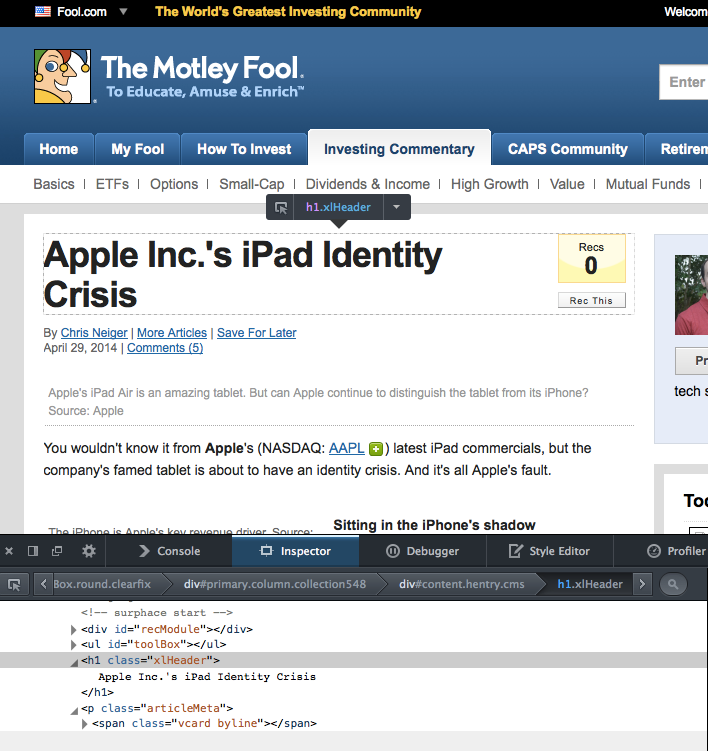
\includegraphics[scale=0.4]{Locator_002}
	\caption{Retrieving the title.}\label{fig:Locator_002}
\end{figure}
	
	\item After this, we would like to know the location of the content of the news article. Here, again \emph{div.entry-content} is a unique location the webpage, or if we want to be more specific, we would write: \emph{body-$>$div.entry-content} as shown in figure \ref{fig:Locator_003}.

\begin{figure}\centering
	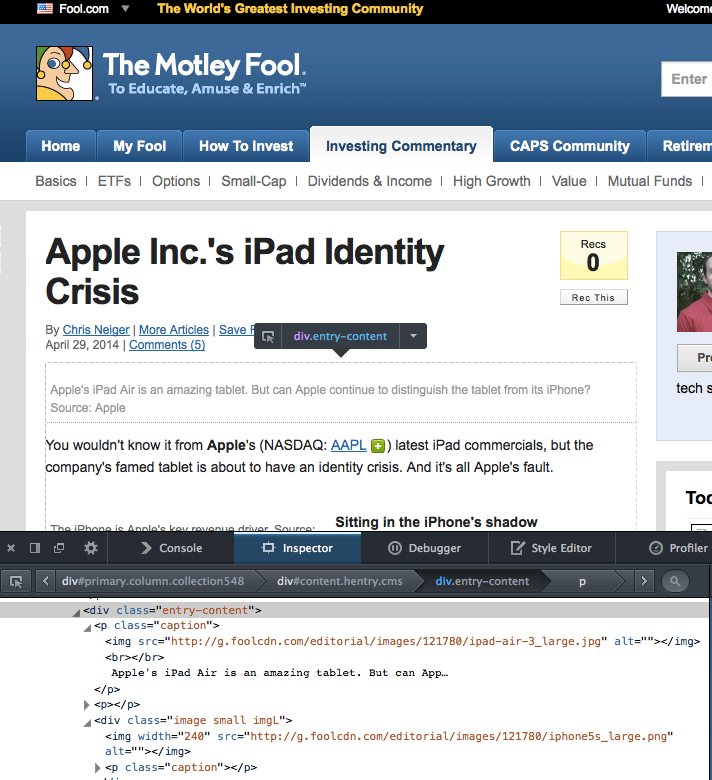
\includegraphics[scale=0.4]{Locator_003}
	\caption{Retrieving the content.}\label{fig:Locator_003}
\end{figure}

	\item Another important thing is the date of the article; as show in the figure \ref{fig:Locator_004}, in order to identify the location of the tag, we must define it as follow: \emph{body-$>$p.articleMeta-$>$span.datetime}.
	
\begin{figure}\centering
	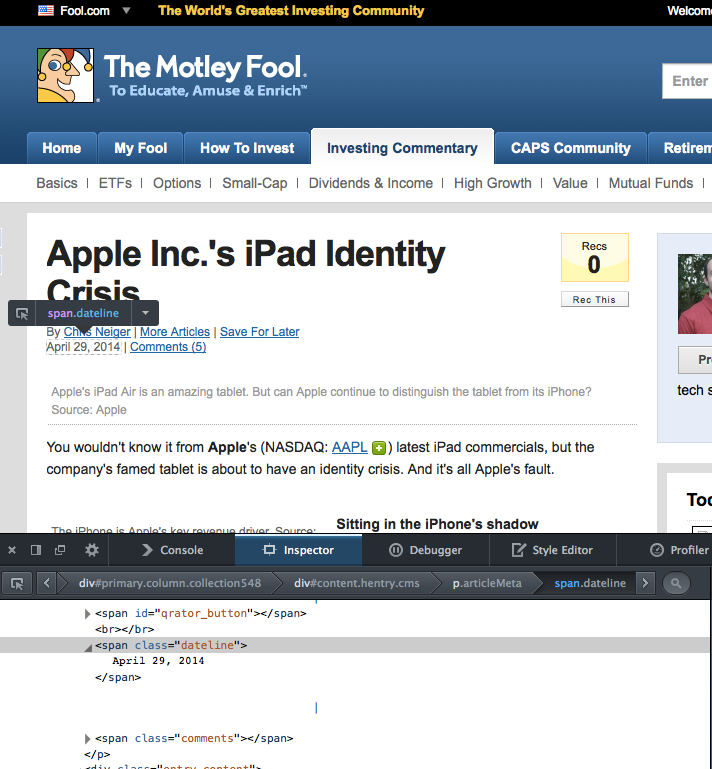
\includegraphics[scale=0.4]{Locator_004}
	\caption{Retrieving the date.}\label{fig:Locator_004}
\end{figure}
	
	\item And last but not least, the author; we must identify the location in the content of the document. Which according to the figure \ref{fig:Locator_005} is: \emph{body-$>$span[itemprop=author]}.
	
\begin{figure}\centering
	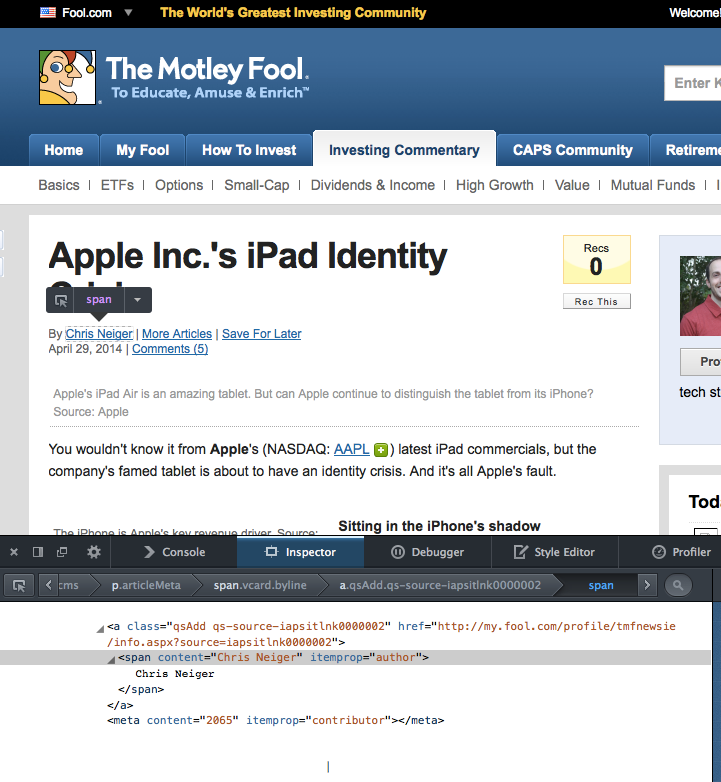
\includegraphics[scale=0.4]{Locator_005}
	\caption{Retrieving the author.}\label{fig:Locator_005}
\end{figure}
	
\end{itemize}

\subsubsection{Generic Locator}\label{genericLocator}

When we think about the scalability of the locators (\ref{locators}), is quite poor; not because it does not fulfil its purpose, but because for every site, we \emph{must} examine the structure of the web page, and this \emph{manual} task takes around 5-10 minutes per site. And, while more news sources we would like to have, more time we should spend constructing our locators. 

So, we have to come out with another method, that allow us to retrieve news article from different sources without spending time examining the structure of every news provider. For us, this method will be called \emph{Generic Locators}. 

To implement this method we will refer first to the section \ref{webCrawler}, and we will take advantage that we already know the date, and title of the article. So we will perform a simple heuristic that will let us retrieve significantly more articles; around 40 \% (According experimental results) if we compare it with the total number of articles retrieved.

As usual, when heuristics are applied, we have to do some trade-off in order to get a good solution with an specific algorithm. In our case, our trade-off will be the accuracy of the text of the article; because sometimes we will get some undesirable characters/phrases in the content of the article. Everything will depend on homogeneous and uniform the structure of the webpage is.

\begin{figure}\centering
	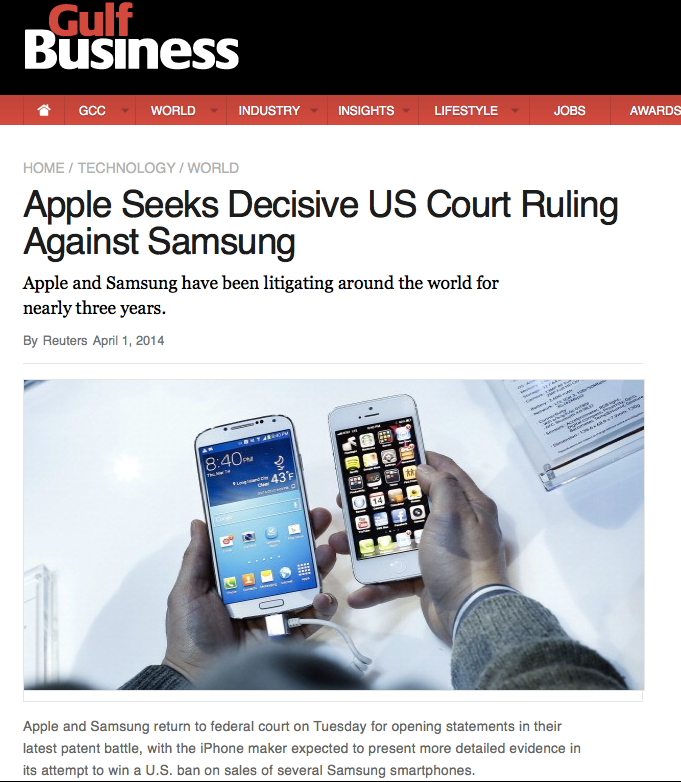
\includegraphics[scale=0.4]{GenericLocator_1}
	\caption{Web page without Locator defined}\label{fig:GL_1}
\end{figure}

We will state an example in order to make it clear. Let's consider this link \url{http://gulfbusiness.com/2014/04/apple-seeks-decisive-us-court-ruling-samsung/} (Figure: \ref{fig:GL_1}). So far, we have implemented a Locator in order to crawl this host and gain 100\% of accuracy. So, in this case that's when the \emph{Generic Locator} comes to play. The text that a \emph{Locator} would retrieve would be the following: 
\\\\
\emph{"Apple and Samsung return to \textbf{federal court} on Tuesday for opening statements in their latest patent battle, with the iPhone maker expected to present \textbf{more detailed} evidence in its attempt to win a U.S. ban on sales of several Samsung smartphones.Apple Inc and Samsung Electronics Co (...)
% Ltd have been litigating around the world for nearly three years. Jurors awarded the iPhone maker about \$930 million after a 2012 trial in San Jose, California, but Apple failed to persuade U.S. District Judge Lucy Koh to issue a \textbf{permanent injunction} against the sale of Samsung phones.A sales ban would be a far \textbf{more serious} threat to Samsung, which earned \$7.7 billion in the quarter that ended in December. Samsung’s \textbf{mobile division}, which includes smartphones, generated operating profit of 5.47 trillion won (\$5.1 billion).The two companies are set to embark on another trial in San Jose over a \textbf{fresh batch} of Apple patents, which cover iPhone features like slide to unlock and search technology. Apple is seeking to ban sales of several Samsung phones, including the Galaxy S III.Likewise, Samsung claims Apple violated two of its patents, and is seeking to ban the iPhone 5. Samsung’s phones use the Android operating system developed by Google Inc.In rejecting Apple’s \textbf{previous bid} for a sales ban, Koh wrote that a consumer survey Apple submitted in the 2012 trial \textbf{likely inflated} the value that customers place on the smartphone features in dispute, meaning Apple does \textbf{not merit} an injunction. Apple is appealing that decision.Apple has hired the \textbf{same marketing} expert to conduct a \textbf{new consumer} survey for the \textbf{current trial}. But this latest effort contains \textbf{additional analysis} about how Apple’s patented features drive consumer demand, according to court filings.While the \textbf{prior survey} \textbf{only concluded} that there was \textbf{general demand} for the patented features, the \textbf{new study} attempts to quantify the proportion of customers Samsung would have lost if its smartphones did \textbf{not contain} those features, court filings show.Samsung tried to stop Apple from presenting that evidence to the jury, arguing that the methodology was unsound. 
However, Koh agreed in a February ruling to allow Apple to use the study.The trial is expected to last until early May.The case in U.S. District Court, Northern District of California is Apple Inc vs Samsung Electronics Co Ltd, 12-630."}
\\\\
And in the case of the generic locator we got: 
\\\\
\emph{\ul{Home \/ Technology \/ World Apple Seeks Decisive US Court Ruling Against Samsung Apple and Samsung have been litigating around the world for nearly three years. By Reuters April 1, 2014} Apple and Samsung return to \textbf{federal court} on Tuesday for opening statements in their latest patent battle, with the iPhone maker expected to present \textbf{more detailed} evidence in its attempt to win a U.S. ban on sales of several Samsung smartphones.Apple Inc and Samsung Electronics Co  (...)
% Ltd have been litigating around the world for nearly three years. Jurors awarded the iPhone maker about \$930 million after a 2012 trial in San Jose, California, but Apple failed to persuade U.S. District Judge Lucy Koh to issue a \textbf{permanent injunction} against the sale of Samsung phones.A sales ban would be a far \textbf{more serious} threat to Samsung, which earned \$7.7 billion in the quarter that ended in December. Samsung’s \textbf{mobile division}, which includes smartphones, generated operating profit of 5.47 trillion won (\$5.1 billion).The two companies are set to embark on another trial in San Jose over a \textbf{fresh batch} of Apple patents, which cover iPhone features like slide to unlock and search technology. Apple is seeking to ban sales of several Samsung phones, including the Galaxy S III.Likewise, Samsung claims Apple violated two of its patents, and is seeking to ban the iPhone 5. Samsung’s phones use the Android operating system developed by Google Inc.In rejecting Apple’s \textbf{previous bid} for a sales ban, Koh wrote that a consumer survey Apple submitted in the 2012 trial \textbf{likely inflated} the value that customers place on the smartphone features in dispute, meaning Apple does \textbf{not merit} an injunction. Apple is appealing that decision.Apple has hired the \textbf{same marketing} expert to conduct a \textbf{new consumer} survey for the \textbf{current trial}. But this latest effort contains \textbf{additional analysis} about how Apple’s patented features drive consumer demand, according to court filings.While the \textbf{prior survey} \textbf{only concluded} that there was \textbf{general demand} for the patented features, the \textbf{new study} attempts to quantify the proportion of customers Samsung would have lost if its smartphones did \textbf{not contain} those features, court filings show.Samsung tried to stop Apple from presenting that evidence to the jury, arguing that the methodology was unsound. 
However, Koh agreed in a February ruling to allow Apple to use the study.The trial is expected to last until early May.The case in U.S. District Court, Northern District of California is Apple Inc vs Samsung Electronics Co Ltd, 12-630. \ul{Get your Free Gulf Business Newsletter}}
\\\\
In the last article we can observe the underlined text, which corresponds to the extra-text retrieved by the \emph{heuristic method (Generic Locator)}. And the text in the bold letters represents the part of speech extracted from the text, in this case doesn't affect the \emph{polarity} of the document. For the first document we had a negative score: -1.06451389862862 and for the second one 0.33956281372088865, according to the equations \ref{eq:ourRange1} and \ref{eq:ourRange2} that defines the criteria to assign the polarity to a document. In this case, both documents have \emph{negative polarity}; but why the different scores for each document if both of them states "almost" the same? The answer to this question is quite simple in this case, the word that makes the biggest impact of the score is on the underlined part of the second document: \ul{Get your \emph{Free} Gulf Business Newsletter}. If we check our file of \emph{positve bag of words}  \cite{M1995} in the line 797, there is the word \emph{Free} which is considered as part of the analysis and it will contribute to the average result in a positive way.
\\\\
We will now describe the \emph{Generic locator algorithm} (\ref{genericLocatorAlgorithm}), which basically takes the \emph{title, date, link and host} and verify if there is an actual locator that can process the web page accurately, then we must check if the link is already in our \emph{page repository}, after this, we will download the article and find the \emph{tag} that contains the \emph{title}, if we found it we will assign the \emph{tag} as \emph{parent} and we will iterate until we fulfill the condition of the \emph{minimum article lenght} (determined experimentally; around 200 characters) and on every iteration we will prepare for the next one, we will assign to the variable \emph{article\_text} the text of the current parent and to \emph{article\_length} the length of the parent, and we will update the \emph{parent} to its \emph{parent}.

\begin{algorithm}
\caption{Generic locator algorithm}\label{genericLocatorAlgorithm}
\begin{algorithmic}[1]

\STATE Input: companyId, title, date, link, host;
\STATE Output: article\_text;
\STATE $article\_lenght \gets 0$;
\STATE $article\_text \gets NULL$;
\STATE $min\_article\_lenght \gets 0$;
\STATE $parent \gets NULL$;
\STATE $tag \gets NULL$;

\IF{\neg $host\_has\_locator}
	\IF{\neg $is\_link\_saved}
		\STATE download \emph{article};
		\STATE find \emph{tag} that contains \emph{title};
		\IF{is\_tag\_found}
			\STATE $parent \gets tag$;
			\WHILE{$article\_lenght < min\_article\_lenght$} 
				\STATE $article\_text \gets parent.text()$
				\STATE $article\_lenght \gets length(article\_text)$
				\STATE $parent \gets parent.parent()$
			\ENDWHILE		
		\ELSE
			\RETURN \emph{NULL};
		\ENDIF
	\ENDIF
\ENDIF
\RETURN $article\_text;

\end{algorithmic}
\end{algorithm}

\subsubsection{Page repository}\label{pageRepository}
Once that the page is fetch and parsed, according to Liu \cite%[p. 321]
{L2011}, it may be stored/indexed. In our case, we will need such a particular repository. Mostly because we are not interested in the web page \emph{per se}, but in its content; as we mention in the subsection \ref{locators}. We could have chosen any particular storage method; file system, document oriented database, object oriented database, but for the purposes of this work we will use a relational database: MySQL because for the following reasons:

\begin{itemize}
    \item The information that we are interested in, is just text.
    \item Several transactions will be executed simultaneously.
    \item Complex queries will be performed.
    \item Stored procedures capabilities.
    \item Summarisation operations will be performed quite often.
\end{itemize}

The database server has the following characteristics:

\begin{itemize}
    \item Server: Localhost via UNIX socket
    \item Software: MySQL
    \item Software version: 5.5.29 - Source distribution
    \item Protocol version: 10
    \item Server charset: UTF-8 Unicode (UTF8)
\end{itemize}

For all the news articles that will be saved in the database, it is important to clarify that no HTML will be stored, mostly because it is not the aim of the work. We will be saving the following fields: Title of the article, content of the article, link, post date, author (not mandatory) and web site. Basically we will index the database by link and by post date of the article. If in the future the original article needs to be checked, the link will be stored.

\subsubsection{Concurrency}\label{concurrency}

Once again, we will make a reference to Liu, \cite%[p. 322]
{L2011}. A crawler basically consumes three main resources: network, CPU and disk. 

In the previous sections we have described basically a sequential crawler, and of course, even if we are really good programmers, and we manage to develop and implement an optimum algorithm, as we mention in the last paragraph, there will be some parameters that will make a bottleneck of our sequential application. 



To state an example we will assume the following: 
\begin{itemize}
    \item A web page that weights around 800 KB
    \item a connection of 256 Kbps
\end{itemize}

According to the figure \ref{fig:Bandwidth} in which we have represented the average download time without considering the \emph{overhead}, it will take around 25 seconds. We could think that this download time is not that bad if we try to download only several web pages; but if we think about it deeply, when we try to download maybe hundreds, thousands or maybe millions, this 25 seconds become a huge overhead. And even for the one page case, this 25 seconds for the processor/CPU seems like ages of waiting, and it will depend on the number of cycles per seconds that the CPU can process, in the example in the table: \ref{tab:downloadIdleness} we have consider a single CPU of 2 GHz (2,000,000,000 cycles every second), and as we can see the idleness of the processor (assuming that the processor is not doing anything else but processing our download request) is quite big and it decreases while we have a faster download speed, but even with today's highest commercial bandwidths available, the idleness of the CPU would be quite high.

\begin{table}\centering
	\caption{Download time \& CPU Idleness}\label{tab:downloadIdleness}
   	\begin{tabular}{ | p{2.5cm\textwidth} | p{3cm\textwidth} | p{3.5cm\textwidth} |}
   	\hline
   	\textbf{Bandwidth (Kbps)}  & \textbf{Download time (seconds)} & \textbf{CPU Idleness (Cycles/second)}  \\ \hline

	9.66&666&1,332,000,000,000\\ \hline
	14.4&441&882,000,000,000\\ \hline
	28.8&222&444,000,000,000\\ \hline
	33.6&190&380,000,000,000\\ \hline
	56&114&228,000,000,000\\ \hline
	64&100&200,000,000,000\\ \hline
	128&50&100,000,000,000\\ \hline
	256&25&50,000,000,000\\ \hline
	512&12&24,000,000,000\\ \hline
	1024&6&12,000,000,000\\ \hline

    \end{tabular}
\end{table}

According to Liu \cite%[p. 322]
{L2011}: the most straightforward way to \emph{speed-up} a crawler is through concurrent processes or threads. Multiprocessing may be somewhat easier to implement than multithreading depending on the programming language and platform.

\begin{figure}\centering
	\caption{Web page download}\label{fig:Bandwidth}
	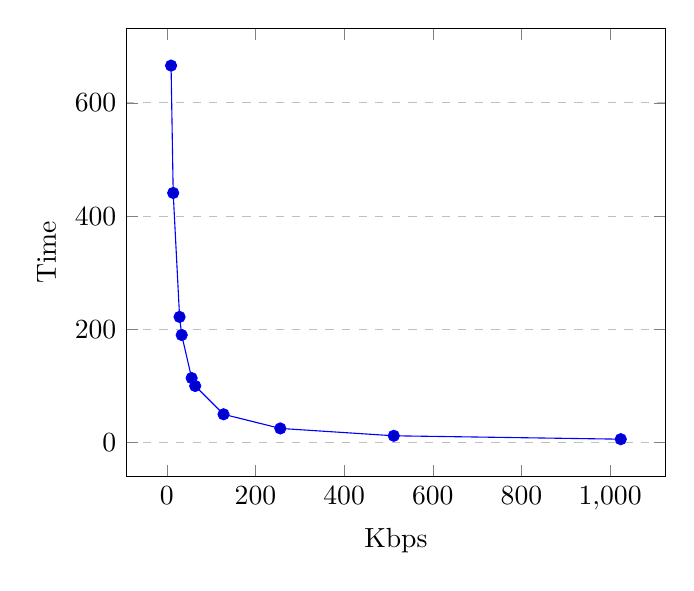
\begin{tikzpicture}
		\begin{axis}[ 
			xlabel=Kbps,
			ylabel=Time,
			ymajorgrids=true,
			grid style=dashed,
  				]	 
			\addplot coordinates {
				(9.6, 666 )
				(14.4, 441)
				( 28.8, 222 )
				(33.6, 190 )
				(56, 114)
				(64, 100)
				(128, 50)
				(256, 25)
				(512, 12)
				(1024, 6)
				};
		\end{axis}
	\end{tikzpicture}
\end{figure}


\begin{figure}\centering
	\caption{CPU Idleness}\label{fig:CPUIdleness}
	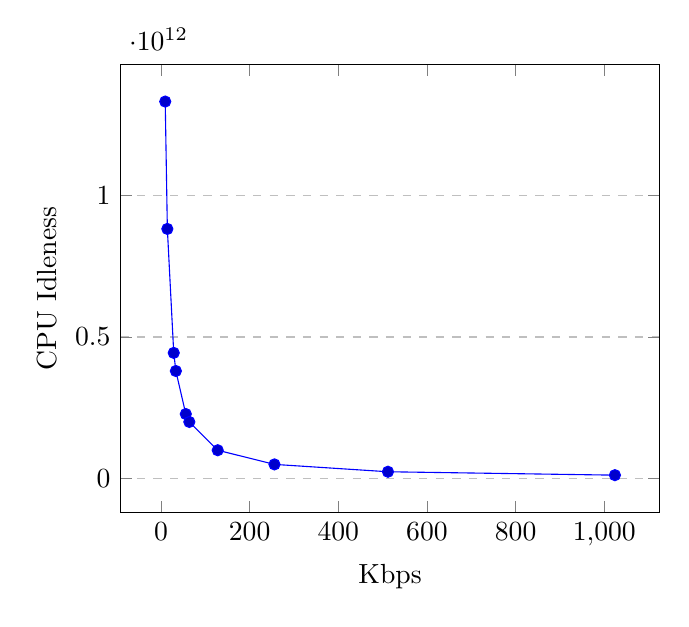
\begin{tikzpicture}
		\begin{axis}[ 
			xlabel=Kbps,
			ylabel=CPU Idleness,
			ymajorgrids=true,
			grid style=dashed,
  				]	 
			\addplot coordinates {
				(9.6, 1332000000000 )
				(14.4, 882000000000)
				( 28.8, 444000000000 )
				(33.6, 380000000000 )
				(56, 228000000000)
				(64, 200000000000)
				(128, 100000000000)
				(256, 50000000000)
				(512, 24000000000)
				(1024, 12000000000)
				};
		\end{axis}
	\end{tikzpicture}
\end{figure}

This word for us (\emph{speed-up}) will have a deeper meaning in the chapter \ref{experimentalEvaluation}, where we will show experimentally the decrease of the idleness of the CPU and the threshold of the parallelisation of the crawler.

In our particular case, we have to make reference to the sequential solution which basically iterates every company until it reaches the last one, after this the collected information is summarised. This approach has the worst time execution (remember: \ref{ParTime}), but of course the best efficiency (remember: \ref{ParEfficiency}); this is represented in the figure \ref{fig:Sequential_1}.

When we will talk about the parallel solution, we will create a pool of requests where we will push the tasks for every company and the framework itself will identify the number of processors available, and it will start to process a set of requests according to the hardware resources available; then it will wait until the last company is processed; this is related to the concept of \emph{Barrier synchronization} (\ref{BarrierSynchronization}). In this case, there will be a threshold where the time will be the best and the speedup as well will be the best; this will be demonstrated experimentally in the chapter \ref{experimentalEvaluation} in the section \ref{MultiThreadingPerformance} specifically in the table \ref{tab:threadsTime}. The idea of the parallel algorithm is depicted in the figure: \ref{fig:Concurrency_1}, and the pseudocode is described in the algorithm \ref{parallelCrawlerAlgorithm} which is implemented in the file \emph{CrawlerThreadPool.java}, this will be the starting point of the console application.

\begin{algorithm}
\caption{Parallel Crawler Algorithm}\label{parallelCrawlerAlgorithm}
\begin{algorithmic}[1]
\STATE \text{Initialize the thread pool;}
\STATE \text{Insert the companies in the thread pool;}
\FORALLP {\text{companies}}
	\STATE \text{Apply the general sequential algorithm \ref{generalAlgorithm};}
\ENDFOR
\STATE \text{Wait until the last task is done (Barrier \ref{BarrierSynchronization}) ;}
\STATE \text{Summarize} \textit{articles}\text{;}
\STATE \text{Download \& Save} \textit{stock prices}\text{;}
\end{algorithmic}
\end{algorithm}


\begin{figure}\centering
	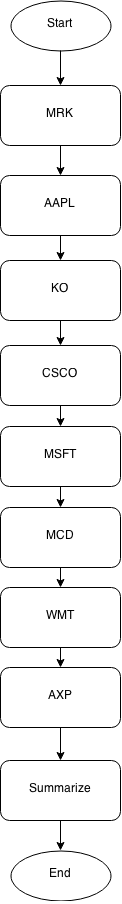
\includegraphics[scale=0.4]{Sequential}
	\caption{Sequential diagram}\label{fig:Sequential_1}
\end{figure}

\begin{figure}\centering
	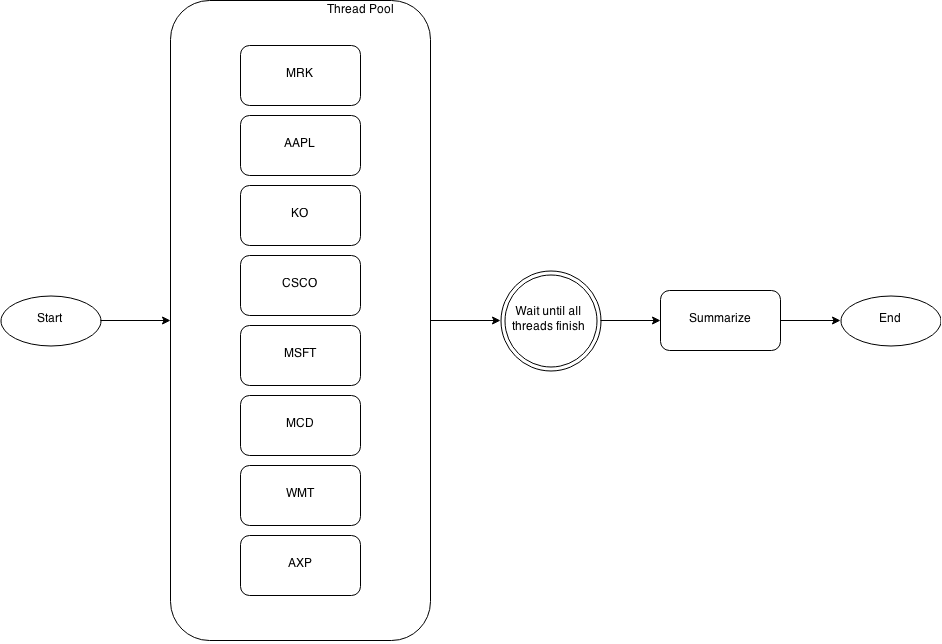
\includegraphics[scale=0.4]{Concurrency}
	\caption{Model of the parallel solution.}\label{fig:Concurrency_1}
\end{figure}



		
		%%%%%%%%%%%%%%%%%%%%%%%%%%%
%%%%%%SENTIMENT ANALYSIS%%%%%%%%
%%%%%%%%%%%%%%%%%%%%%%%%%%%
\clearpage
\section{Sentiment analysis}\label{sentimentAnalysis}

In this section we will describe the algorithms and conventions that were used in order to perform the Sentiment analysis. The implementation can be found in the file "PolarityAnalysis.java".
This part may be considered as the most important of the work, because the results that will be presented will be based on the data produced by polarity analyzer that we will describe on this section.

Up to this point, we already have the results of crawler, from the point of view of the Sentiment analysis this will be the input data. The task that we will perform in this chapter could be seen as "simple" or "trivial", because for a person is quite normal to read an article and decide if the article has positive or negative polarity.

But what if, instead of only one article we have ten, one hundred, one thousand, ten thousands, or we may say \textit{"N"} articles every day and our task would be to classify all this documents.

Now the situation becomes a bit more complicated, because with the previous method (read and classify manually) would be expensive to pay hundreds of people in order to read and decide about the polarity of this \textit{"N"} articles, besides all of them will apply its own criteria. \cite%[p. 459]
{L2011} Because usually people pay more attention with text or opinions that are consistent with their own preferences.

Basically, what we will be doing is a statistical analysis of some particular article, according to some parameters that we will define in this chapter, and after this we will assign a score to the document, and depending on this score, the article will be classified as positive or negative. But before all of this, we will explore Opinion Mining/Sentiment analysis more deeper in order to understand better this techniques. 

\subsection{Document sentiment classification}\label{documentSentimentClasification}

Now that we describe the general aim of this chapter, we will start to scratch a bit deeper, we will focus according to Liu \cite%[p. 469]
{L2011} in one of the main research topics of opinion mining; \textit{sentiment clasification}, it classifies a document as expressing a positive or negative opinion/sentiment. This particular task, is known as document-level sentiment classification because it considers the whole document as the basic information unit. 

In order to get to our point (Sentiment analysis), we need to define several important concepts: opinion and the problem of sentiment classification.

\begin{itemize}
	\item Entity: This could be a product, service, person, event, organisation, or topic.
	\item Aspect: Are the components and attributes of an Entity.
	\item Aspect name: An aspect name is the name of an aspect given by the user.
	\item Aspect expression: is an actual word or phrase that has appeared in text indicating an aspect.
	\item Entity name: An entity name is the name of an entity given by the user.
	\item Entity expression: is an actual word or phrase that has appeared in text indicating an entity.
	\item Opinion holder: The holder of an opinion is the person or organisation that expresses the opinion.
\end{itemize}

\subsubsection{Opinion}\label{opinion}
As our common sense would tell us, an opinion from an entity could be rather positive or negative and it can contain emotions, attitude or appraisal.
To positive and negative, we will call them opinion orientations; this are called as well: sentiment orientation, semantic orientation or polarity.
After mentioning a concept about "opinion" we will define it formally according to Liu \cite%[p. 463]
{L2011}. Basically it is a quintuple:

\begin{equation} \label{eq:opinionQuintuple}
	\textit{(e\textsubscript{i}, a\textsubscript{ij}, oo\textsubscript{ijkl}, h\textsubscript{k}, t\textsubscript{l})}
\end{equation}


Where \emph{e\textsubscript{i}} is the \textbf{name of an entity}, \emph{a\textsubscript{ij}} is an \textbf{aspect} of \emph{e\textsubscript{i}}, \emph{oo\textsubscript{ijkl}} is the \textbf{orientation of the opinion} about the aspect \emph{a\textsubscript{ij}} of entity \emph{e\textsubscript{i}}, \emph{h\textsubscript{k}} is the \textbf{opinion holder}, and \emph{t\textsubscript{l}} is the \textbf{time} when the opinion is expressed by \emph{h\textsubscript{k}}.


Now that we define an opinion, we will define a model of entity, a model of opinionated document, and the mining objective, which are collectively called the aspect-based opinion mining.

Model of entity: An entity e\textsubscript{i} (which is a product, service, person, event, organisation, or topic.) is represented by itself as a whole and a finite set of aspects (The aspects of an entity e are the components and at- tributes of e.), A\textsubscript{i} = \{a\textsubscript{i1}, a\textsubscript{i2}, ..., a\textsubscript{in}\}. The entity itself can be expressed with any one of a final set of entity expressions OE\textsubscript{i} = \{oe\textsubscript{i1}, oe\textsubscript{i2}, ..., oe\textsubscript{is}\}. Each aspect a\textsubscript{ij} in A\textsubscript{i} of the entity can be expressed by any one of a finite set of aspect expressions AE\textsubscript{ij} = \{ae\textsubscript{ij1}, ae\textsubscript{ij2}, ..., ae\textsubscript{ijm}\}. (An aspect name is the name of an aspect given by the user, while an aspect expression is an actual word or phrase that has appeared in text indicating an aspect.)


Model of opinionated document: An opinionated document d contains opinions on a set of entities \{e\textsubscript{1}, e\textsubscript{2}, ..., e\textsubscript{r}\} from a set of opinion holders \{h\textsubscript{1}, h\textsubscript{2}, ..., h\textsubscript{p}\}. The opinions on each entity e\textsubscript{i} are expressed on the entity itself and a subset A\textsubscript{id} of its aspects.
                                                                                                                                                                                                                                                                                                                                                                                                                                                                                                                                                                                                                                                                                                                                                                                                                                                                                                                                                                                                                                                                                                                                                                                                                                                                                                                                                                                                                                                                                                                                                                                                                                                                                                                                                                                                                                                                                                                                                                                                                                                                                                                                                                                                                                                                                                                                                                                                                                                                                                                                                                                                                                                                                                                                                                                                                                                                                                                                                                                                                                                                                                                                                                                                                                                                                                                                                                                                                                                                                                                                                                                                                                                                                                                                                                                                                                                                                                                                                                                                                                                                                                                                                                                                                                                                                                                                                                                                                                                                        

To achieve this objective, we need to perform the following tasks:
\begin{itemize}
	\item Task  1 (entity extraction and grouping): Extract all entity expressions in D, and group synonymous entity expressions into entity clusters. Each entity expression cluster indicates a unique entity ei.
	\item Task  2 (aspect extraction and grouping): Extract all aspect expressions of the entities, and group aspect expressions into clusters. Each aspect expression cluster of entity ei indicates a unique aspect aij.
	\item Task  3 (opinion holder and time extraction): Extract these pieces of information from the text or structured data.
	\item Task  4 (aspect sentiment classification): Determine whether each opinion on an aspect is positive, negative or neutral.
	\item Task  5 (opinion quintuple generation): Produce all opinion quintuples \emph{(e\textsubscript{i}, a\textsubscript{ij}, oo\textsubscript{ijkl}, h\textsubscript{k}, t\textsubscript{l})} expressed in D based on the results of the above tasks.
\end{itemize}

We will give an example from an article taken from: \url{http://www.valuewalk.com/2014/04/iphone-6-specs/} and we will follow the task pattern we mention before.

"Published on: 2014-04-05. By: Vikas Shukla. The iPhone 6 may have the fastest Wi-Fi, thanks to the new Wi-Fi chip developed by Apple's partner Broadcom Apple Inc."

\begin{itemize}
	\item Task 1 (entity extraction and grouping): "iPhone"
	\item Task 2 (aspect extraction and grouping): "Wi-Fi"
	\item Task 3 (opinion holder and time extraction): Vikas Shukla / 2014-04-05
	\item Task 4 (aspect sentiment classification): Positive opinion to get a fastest Wi-Fi
	\item Task 5 (opinion quintuple generation): (iPhone, Wi-Fi, positive, Vikas Shukla, 2014-04-05)
\end{itemize}

We already define some basics about opinion mining, as we mention before, our goal will be to classify a  document, and in our particular case will be news articles and express if this article/document is positive or negative. The task of expressing the sentiment/polarity of a document is called: \textbf{document level sentiment classification.} 

For this we will mention the \textbf{problem definition} that is presented on %\cite[p. 469]{L2011} of the author which is: 

\emph{Problem Definition}: Given an \emph{opinionated document} \textbf{d} evaluating an \emph{entity} \textbf{e}, determine the \emph{opinion orientation} \textbf{oo} on \textbf{e}, i.e., determine \textbf{oo} on aspect \emph{General} in the quintuple: (e, h, and t are assumed known or irrelevant)

\begin{equation} \label{eq:documentClassificationProblem}
	(e, General, oo, h, t)
\end{equation}

\emph{Assumption}: Sentiment classification assumes that the \emph{opinion document} d expresses opinions on a single entity e and the opinions are from a single \emph{opinion holder} h.

\subsection{Classification based on unsupervised learning}\label{unsupervisedLearning}

The aim of this section is to explain the algorithm used in order to classify an article. Particularly I had several chats with finance-related people and I mentioned the basic idea of this work; and the common question of all of them was: \emph{"How you/computer will decide if an article is positive or negative?"}. According to this brief survey, I realised that most of people (Non-IT-related) don't realise about "opinion mining" techniques.

We will mention here quite often, the algorithm used by Peter Turney \cite{T2002} which originally was designed to classify movie reviews as recommended or not recommended. We will base on this algorithm with certain modifications in order to achieve our goal (Classify news articles). Basically this kind of algorithms have a simple input and output; if we would see at it as a blackbox it would look like this:


\emph{Text to be analyzed} $\rightarrow $\emph{Algorithm} $\rightarrow$ \emph{Classified text (Positive/Negative)}

\subsubsection{Why Unsupervised learning?}\label{whyUnsupervised}

There are basically two ways how to approach the \emph{document classification: Supervised and Unsupervised Classification}.

This algorithm (Unsupervised Classification) was chosen mostly because of the "Unsupervised" part, because it would be hard to perform some "Supervised learning" mostly because of the time constrains; in which several hundreds of articles must be read and classified "manually", and then apply some machine learning techniques.

\subsubsection{Unsupervised learning algorithm}\label{unsupervisedAlgoritm}

The \emph{unsupervised learning alogorithm} is based on a set of already classified \emph{positive/negative "bag of words"} taken from: \url{http://www.cs.uic.edu/~liub/FBS/sentiment-analysis.html}.

If we would take a simple algorithm like: count the positive and negative words and subtract the positive from the negatives and if the result is positive, then the article is possible; with this algorithm, we would not be considering the relationship of every positive or negative word with its environment. So, our algorithm will be a bit more complicated than that. 

We will use two techniques that belongs to:
	\begin{itemize}
		\item Text mining and natural language processing discipline called \emph{part-of-speech (POS) tagging}
		\item Information theory and statistics which measures association called \emph{Pointwise mutual information - PMI.} (Defined in section: \ref{PMI})
	\end{itemize}

\subsubsection{Part-of-speech tagging}\label{partOfSpeech}

The part-of-speech of a word is a linguistic category that is defined by its syntactic or morphological behaviour. In English; the language of the news articles that we will be analysing, exists seven parts-of-speech, which we will define briefly according to the work of Lyon \cite{L1832}.

	\begin{itemize}
		\item Noun: Name of any person, place, thing, quality, or principle. The name of whatever should be the subject of a conversation.
		\item Adjective: The aim of the adjectives is to designate the noun, or to point some peculiarity belonging to it. In the English language, its position is, and always may be, immediately \emph{before} the noun.
		\item Pronoun: This part of speech is self-explainable. and according to \cite%[p.~31]
		{L1832}  is well named. It is a word used instead of, or for a noun.
		\item Verb: Is the "chief word" in a sentence, and without it, no sentence can be completed. It denotes action or condition of being.
		\item Preposition: It is a primary characteristic is that affects words in contradistinction to sentences; namely, nouns, adjectives, pronouns, and participles; and in particular, any word, not being a verb, which governs the objective case of a pronoun.
		\item Conjunction: It is a primary characteristic is to affect words, and, in particular, to govern the objective case of the pronoun.
		\item Adverb: A word is an adverb when is clear that this word don't belong to any other part of speech. Conjunctions and Interjections can be categorised as Adverbs. Some authors classify this last two in different categories of part-of-speech.
	\end{itemize}
	
After this categorisation, we need to keep in mind that this previously mentioned part-of-speech can be classified deeply. For example, we often can found verbs in its infinitive form, present, past, gerund, etc. For our purposes we will use the Penn Treebank POS Tags as shown in the table \ref{tab:posTags}. \emph{POS tagging} is the task of labelling each word in a sentence with its appropriate part-of-speech. For our analysis, we will use the text mining software GATE, in order to perform the extraction of the phrases that fulfil the criteria defined in the table \ref{tab:twoWordPhrases}. To achieve this, we have to write a jape file named: "patterns.jape", this file contains the specifications defined in the table \ref{tab:twoWordPhrases}; and it looks as follows: 

\begin{lstlisting}
Phase:	PolarityPattern
Input:  Lookup Token
Options: control = brill

Rule: PolarityPattern
Priority: 100
(
 (
   {Token.kind==word, Token.category==JJ}
   {Token.kind==word, Token.category== NN}
 )
 
(...) // In order to exemplify, several conditions have been omitted; anyway, the jape file is valid.

)
:PolarityPattern
-->
{
	// Java code to process the Annotation set.
}
\end{lstlisting}

\begin{table}\centering
	\caption{Penn Treebank Part-Of-Speech (POS) tags}\label{tab:posTags}
   	\begin{tabular}{|l|p{5cm\textwidth}|l|p{5cm\textwidth}|}
   	\hline
   	\textbf{Tag}  & \textbf{Description} & \textbf{Tag}  & \textbf{Description}\\ \hline
	CC &Coordinating conjunction &PRP\$ &Possessive pronoun \\ \hline
	CD &Cardinal number &\textbf{RB} &\textbf{Adverb} \\ \hline
	DT &Determiner &\textbf{RBR} &\textbf{Adverb, comparative} \\ \hline
	EX &Existential there &\textbf{RBS} &\textbf{Adverb, superlative} \\ \hline
	FW &Foreign word &RP &Particle \\ \hline
	IN &Preposition or subordinating conjunction &SYM &Symbol \\ \hline
	\textbf{JJ} &\textbf{Adjective} &TO &to \\ \hline
	JJR &Adjective, comparative &UH &Interjection \\ \hline
	JJS &Adjective, superlative &\textbf{VB} &\textbf{Verb, base form} \\ \hline
	LS &List item marker &\textbf{VBD} &\textbf{Verb, past tense} \\ \hline
	MD &Modal &\textbf{VBG} &\textbf{Verb, gerund or present participle} \\ \hline
	\textbf{NN} &\textbf{Noun, singular or mass} &\textbf{VBN} &\textbf{Verb, past participle} \\ \hline
	\textbf{NNS} &\textbf{Noun, plural} &VBP &Verb, non-3rd person singular present \\ \hline
	NNP &Proper noun, singular &VBZ &Verb, 3rd person singular present \\ \hline
	NNPS &Proper noun, plural &WDT &Wh-determiner \\ \hline
	PDT &Predeterminer &WP &Wh-pronoun \\ \hline
	POS &Possessive ending &WP\$ &Possessive wh-pronoun \\ \hline
	PRP &Personal pronoun &WRB &Wh-adverb \\ \hline
    \end{tabular}
\end{table}

\begin{table}\centering
	\caption{Patterns of tags for extracting two-word phrases}\label{tab:twoWordPhrases}
   \begin{tabular}{|l|l|l|}
   	\hline
   	\textbf{ }  & \textbf{First word}  & \textbf{Second word} \\ \hline
	1&JJ &NN or NNS \\ \hline
	2&RB, RBR, or RBS &JJ \\ \hline
	3&JJ &JJ \\ \hline
	4&NN or NNS &JJ \\ \hline
	5&RB, RBR, or RBS &VB, VBD, VBN, or VBG \\ \hline
    \end{tabular}
\end{table}
\pagebreak
We will show a small example how to use this jape file using the GATE User Interface, in order to get the desired results and to prove that it works. In order to make this example work, we will use one phrase from link in the previous example: \url{http://www.valuewalk.com/2014/04/iphone-6-specs/} as shown in figure \ref{fig:POS1}, and we will follow the next steps:

	\begin{itemize}
		\item Open GATE (Figure \ref{fig:POS2})
		
			\begin{figure}\centering
				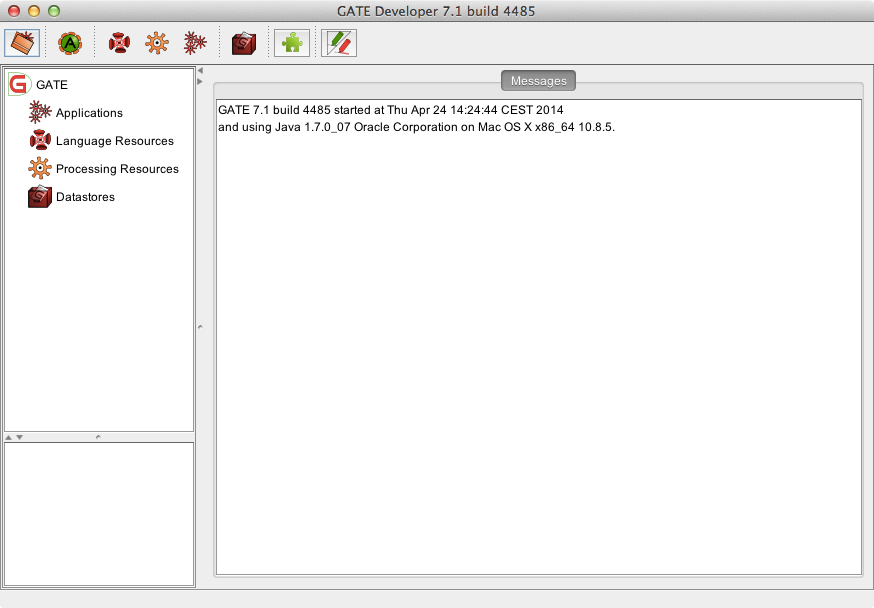
\includegraphics[scale=0.4]{POS2_Gate_nic}
				\caption{Gate interface}\label{fig:POS2}
			\end{figure}
		
		\item Consider the following text: \\\\"Apple Inc. (NASDAQ:AAPL) has announced that the Worldwide Developers Conference (WWDC) will begin on June 2. But the company is unlikely to launch the iPhone 6 at the event. The latest rumours suggest that the iPhone 6 will enter production in May and reach the public in September. As rumours build up ahead of its launch, consumers will wait for the upcoming iPhone rather than buying the current models. Let’s explore some of the latest rumours targeting its features, specifications and technologies." (Figure \ref{fig:POS1})
		
			\begin{figure}\centering
				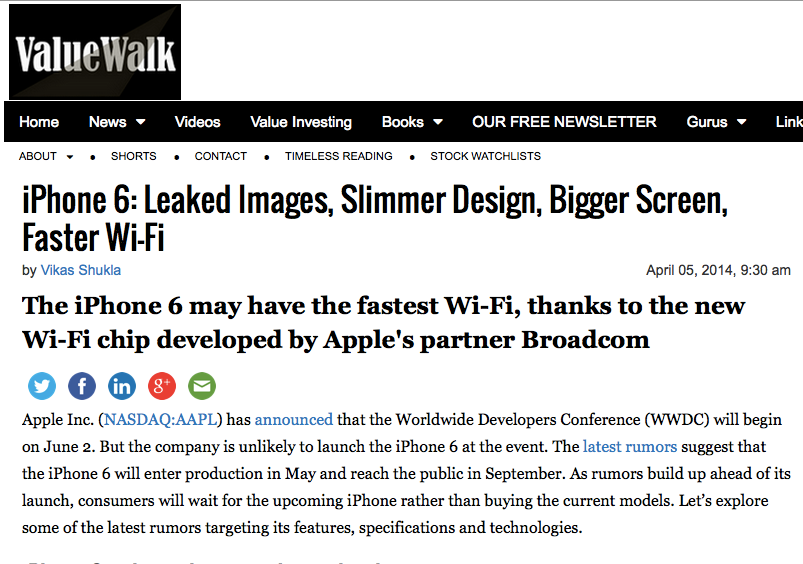
\includegraphics[scale=0.45]{POS1}
				\caption{Web page that contains the text to analyze}\label{fig:POS1}
			\end{figure}
		
		\item In "Processing Resources" add the following elements: Document reset, Tokeniser, sentence splitter, POS tagger and JAPE transducer (Don't forget to look for the "pattern.jape" file). (Figure \ref{fig:POS3}, \ref{fig:POS4})
		
			\begin{figure}\centering
				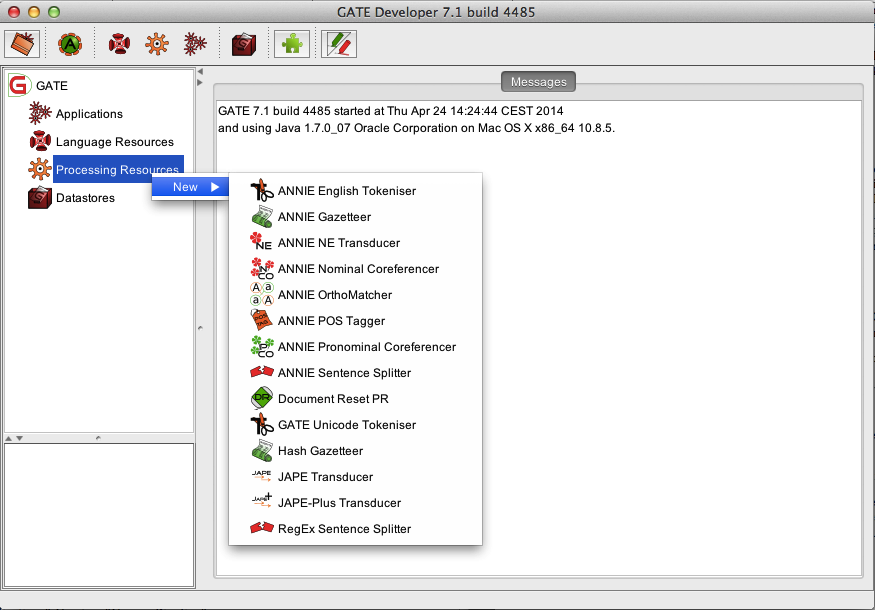
\includegraphics[scale=0.4]{POS3_Gate_processingResources}
				\caption{Processing resources available}\label{fig:POS3}
			\end{figure}

			\begin{figure}\centering
				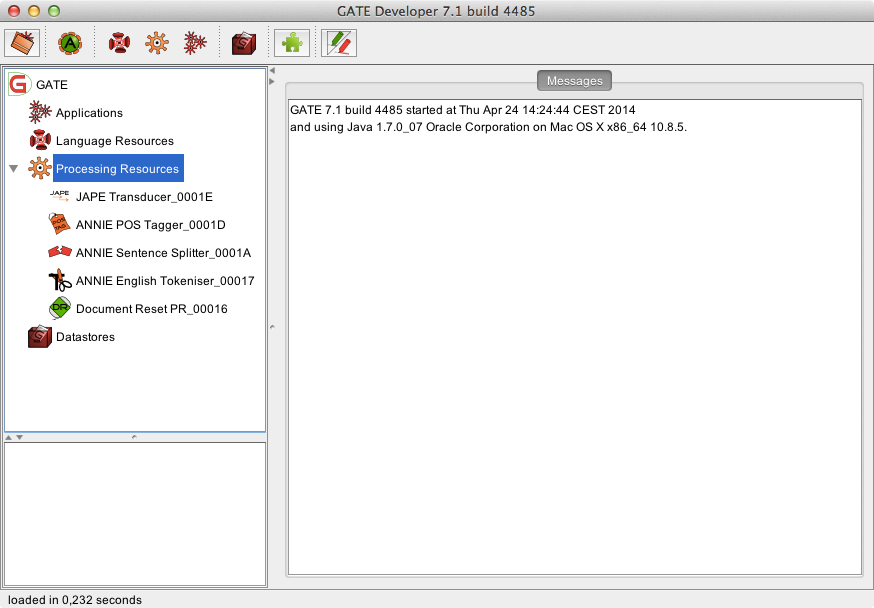
\includegraphics[scale=0.4]{POS4_Gate_ProcessingResources_2}
				\caption{Processing resources needed}\label{fig:POS4}
			\end{figure}
		
		\item In "Languages Resources" Create a "Corpus". (Figure \ref{fig:POS5})
		
			\begin{figure}\centering
				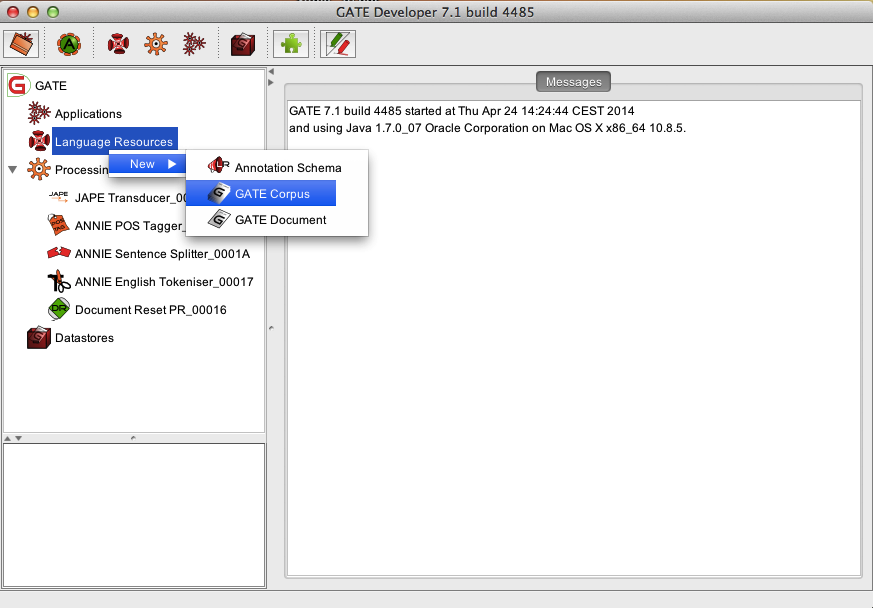
\includegraphics[scale=0.4]{POS5_Gate_LanguateResources_1}
				\caption{Language resources, Corpus \& Document}\label{fig:POS5}
			\end{figure}
		
		\item In "Languages Resources" Create a "Document". (Figure \ref{fig:POS6})
		\item Open the "Document" and paste the text that we are considering. (Figure \ref{fig:POS6})
		
			\begin{figure}\centering
				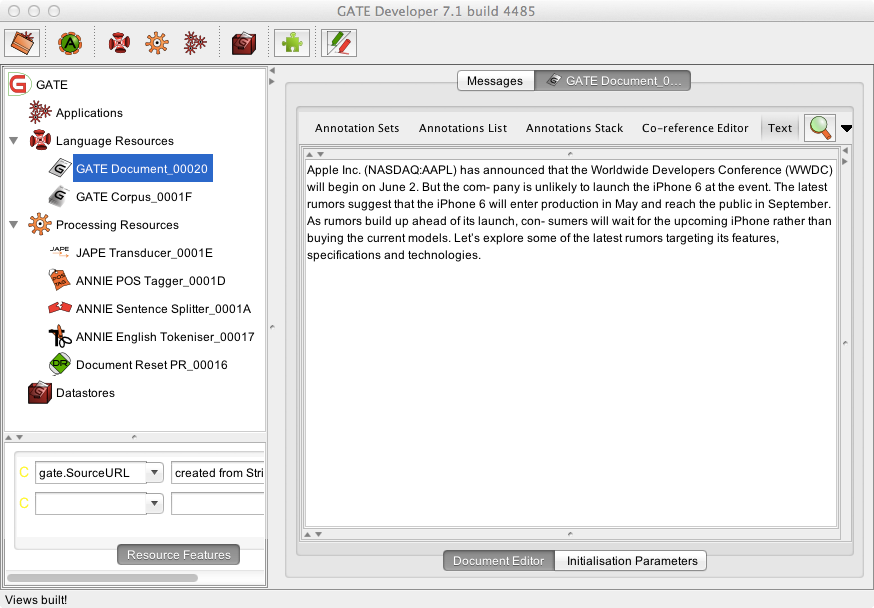
\includegraphics[scale=0.4]{POS6_Gate_LanguateResources_2}
				\caption{Language resources, Text processing}\label{fig:POS6}
			\end{figure}
		
		\item Open the "Corpus" and drag and drop the "Document" to the corpus working area. (Figure \ref{fig:POS7})
		
			\begin{figure}\centering
				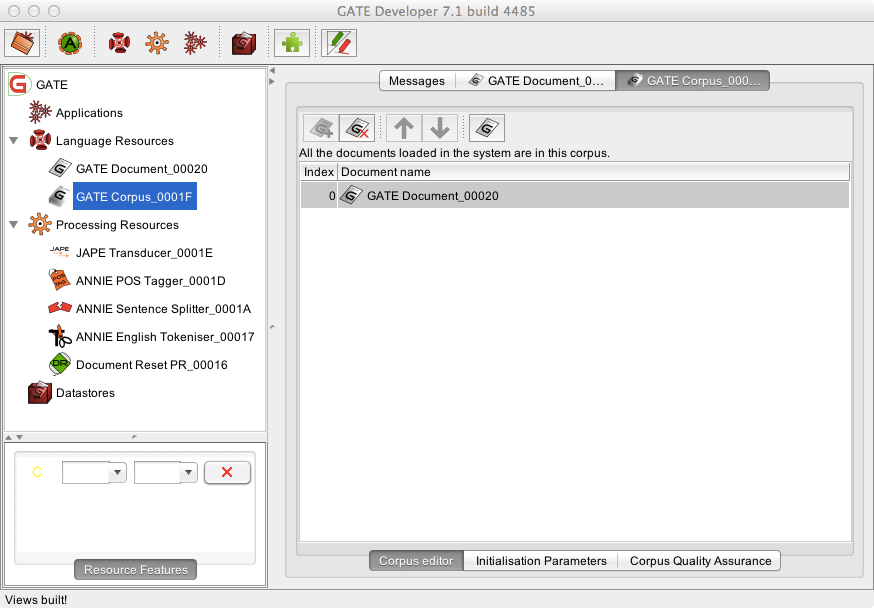
\includegraphics[scale=0.4]{POS7_Gate_LanguateResources_3}
				\caption{Language resources, Document drag \& drop to Corpus area}\label{fig:POS7}
			\end{figure}
		
		\item In "Applications" Create a "Corpus Pipeline" (Figure \ref{fig:POS8})
		
			\begin{figure}\centering
				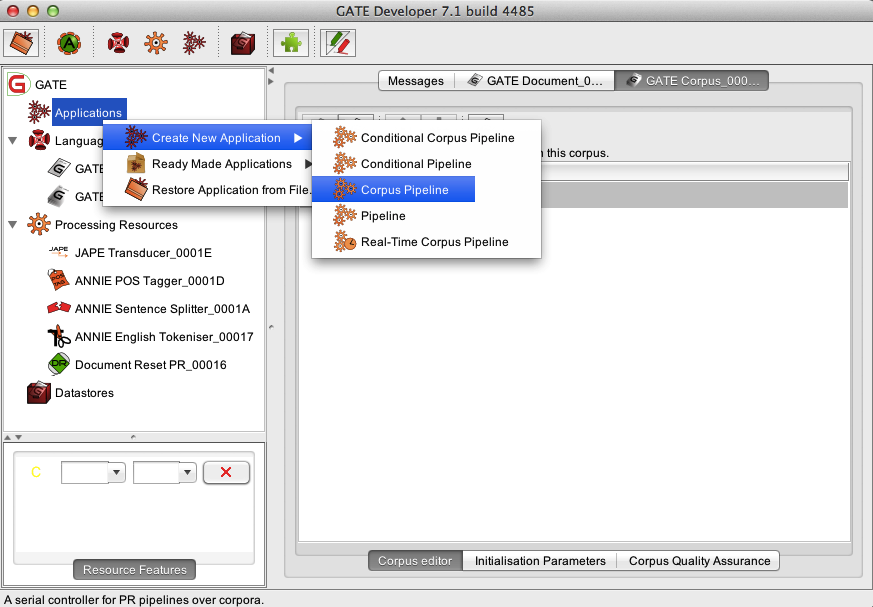
\includegraphics[scale=0.4]{POS8_Gate_Applications_1}
				\caption{Corpus creation}\label{fig:POS8}
			\end{figure}
		
		\item Open the "Corpus Pipeline", select the created "Corpus" and add the processing resources in the following order: Document reset, Tokeniser, sentence splitter, POS tagger and JAPE transducer. (Figure \ref{fig:POS9})
		
			\begin{figure}\centering
				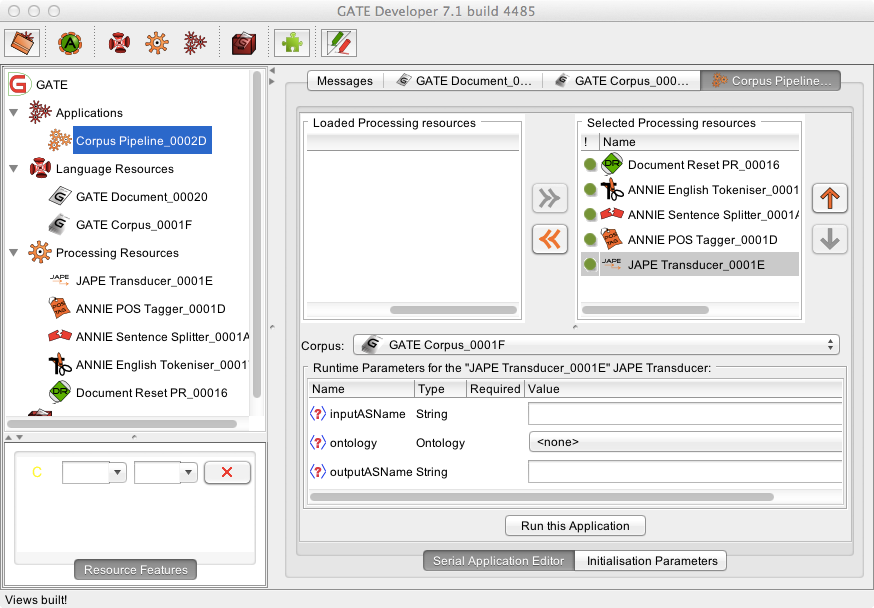
\includegraphics[scale=0.4]{POS9_Gate_Applications_2}
				\caption{Corpus setup}\label{fig:POS9}
			\end{figure}
		
		\item Press the "Run this application" button.
		\item Go back to the "Document" and press the buttons: "Annotation Sets" and "Annotation List". (Figure \ref{fig:POS10})
		
			\begin{figure}\centering
				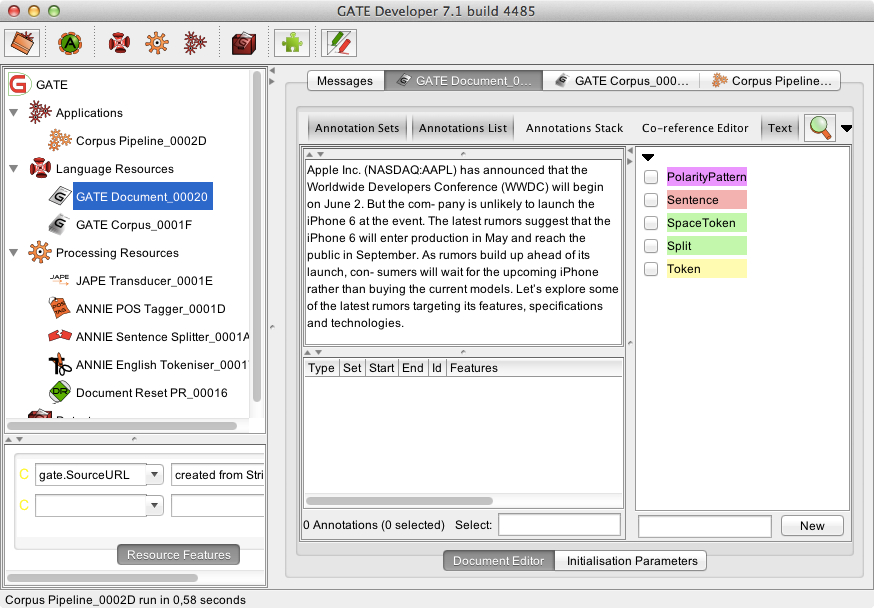
\includegraphics[scale=0.4]{POS10_Gate_Applications_3}
				\caption{Processed Document 1}\label{fig:POS10}
			\end{figure}
		
		\item After completing the previous step Click on the right: "Polarity Pattern" (Figure \ref{fig:POS10})
		\item We will see in the "Document" text marked as follows: \\\\
		Apple Inc. (NASDAQ:AAPL) has announced that the Worldwide Developers Conference (WWDC) will begin on June 2. But the company is unlikely to launch the iPhone 6 at the event. The latest rumours suggest that the iPhone 6 will enter production in May and reach the public in September. As rumours build up ahead of its launch, consumers will wait for the \textbf{\emph{upcoming iPhone}} rather than buying the \textbf{\emph{current models}}. Let’s explore some of the latest rumours targeting its features, specifications and technologies.
		\item By the time we will be running the algorithm, this two phrases were found and its neighbours words will be considered in order to calculate the polarity of the paragraph/document. (Figure \ref{fig:POS11})
		
			\begin{figure}\centering
				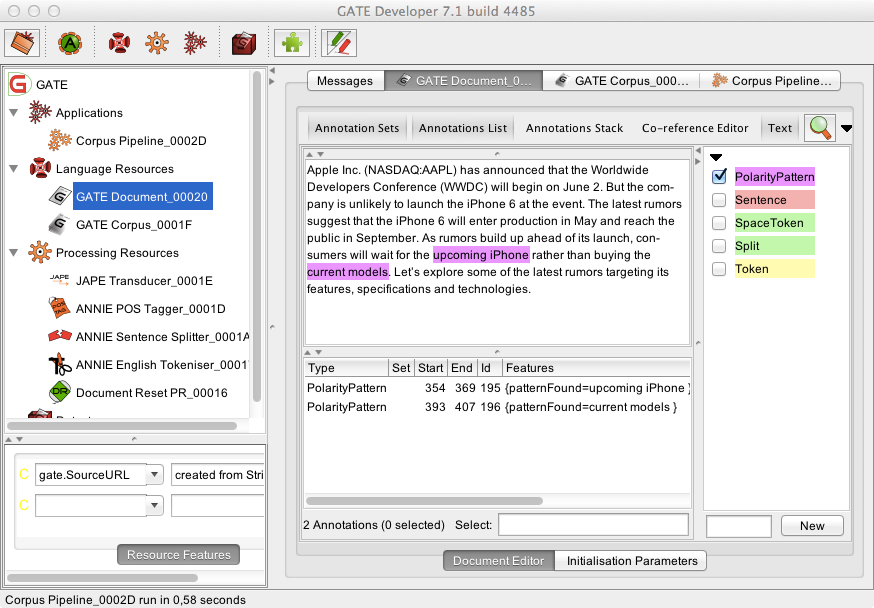
\includegraphics[scale=0.4]{POS11_Gate_Applications_4}
				\caption{Processed Document 2}\label{fig:POS11}
			\end{figure}
		
		\item This two phrases were selected according to the conditions stablished in the table \ref{tab:twoWordPhrases}. \emph{Upcoming} is adjective and \emph{iphone} is noun, and \emph{current} is adjective and \emph{models} is a noun.
	\end{itemize}
	
We already define how we will extract from the text of the article the required part-of-speech, now we will make a reference to the \emph{Pointwise mutual information} which we defined already in the section: \ref{PMI} and according to the obtained data we came to an observation; Usually authors define that reviews or texts with \emph{$PMI > $0} will be classified as \emph{positive} and \emph{$PMI \leq $0} will be classified as \emph{negative}. In this work, according to the meticulous reading of several articles (examples are shown in table: \ref{tab:FalsePositives}); when they have \emph{$0 \leq $PMI \leq $1}, the polarity of this articles even if according to some authors mathematically it is positive, in the majority of the analysed articles, their orientation is quite debatable. And in the case of finance news articles we will consider that an article should be positive enough to be consider as positive as shown in the equations \ref{eq:ourRange1} and \ref{eq:ourRange2}. With this assumption we will avoid to classify as positive anything that could be debatable, and in finances if something is debatable it \emph{should be} negative.

\begin{equation} \label{eq:ourRange1}
	-\infty \leq \operatorname{pmi}(x;y) \leq +1
\end{equation}

\begin{equation} \label{eq:ourRange2}
	+1 < \operatorname{pmi}(x;y) \leq +\infty
\end{equation}


\begin{table}\centering
	\caption{False Positives}\label{tab:FalsePositives}
   	\begin{tabular}{ | p{1.1cm\textwidth} | p{8cm\textwidth} | p{1.5cm\textwidth} | p{1.5cm\textwidth} |}
   	\hline
   	\textbf{Firma}  & \textbf{Title} & \textbf{Date} & \textbf{Score}  \\ \hline

AAPL&Samsung Electronics Co Ltd Wins Bid To Sell Nexus In Apple Inc Court Battle-Reuters&07/07/12&0.584482 \\ \hline
AAPL&Apple Inc Claims \$2.5 Billion Damages In Samsung Electronics Co Ltd Patent Case-Reuters&24/07/12&0.169725 \\ \hline
AAPL&Losers on major news: Microsoft (NASDAQ:MSFT), Citigroup (NYSE:C), Apple (NASDAQ:AAPL), Google (NASDAQ:GOOG)&28/03/14&0.405027 \\ \hline
AXP&US in talks with France on Holocaust compensation&10/04/14&0.655722 \\ \hline
BA&The Boeing Company (BA): Cash Generation May Disappoint Near-Term&13/03/14&0.777058 \\ \hline
BA&Mad Money Recommends Boeing: So Is It Time To Sell?&17/03/14&0.60467 \\ \hline
BA&"UPDATE: Malaysia Airlines MH370: 122 Objects Found In Southern Indian Ocean \& Legal Action Initiated Against Boeing And Malaysia Airlines"&26/03/14&0.705982 \\ \hline
BA&Boeing to Cut 300 Jobs in Australia as Manufacturing Weakens (1)&02/04/14&0.589379 \\ \hline
CSCO&Cisco Should Be Upgraded, Not Downgraded&19/03/14&0.870265 \\ \hline
CSCO&Cisco: Too Little, Too Late?&25/03/14&0.203206 \\ \hline
GE&GM Workers Who Built Defective Cars Fret About Recall&09/01/14&0.309883 \\ \hline
GS&Not a Good Day for Wall Street&08/04/14&0.0616087 \\ \hline
INTC&Is Intel In The Danger Zone?&20/02/14&0.646839 \\ \hline
INTC&Intel: The Worst-Case Scenario&27/02/14&0.368407 \\ \hline
INTC&Even More Bad Luck For Intel?&17/03/14&0.551018 \\ \hline
INTC&Microsoft Office For iPad Is Toxic To Intel&23/03/14&0.326464 \\ \hline
KO&Soda sales rapidly decline across the United States&31/03/14&0.430099 \\ \hline
KO&Soda sales in US drop steadily&03/04/14&0.981124 \\ \hline
MCD&McDonald's COO to retire&20/03/14&0.996407 \\ \hline
MCD&McDonald's Closes Crimean Locations&04/04/14&0.160516 \\ \hline
MCD&McDonald's Pulls Out of Crimea Due to Russian Annexation&05/04/14&0.633011 \\ \hline
    \end{tabular}
\end{table}

\subsubsection{Semantic orientation - SO}\label{SO}

According to Liu \cite%[p. 474]
{L2011},  \emph{semantic orientation} of a phrase is computed based on its association with the positive reference word “excellent” and its association with the negative reference word “poor”:

\begin{equation} \label{eq:SO1}
	SO(phrase) = PMI(phrase, "excellent") - PMI(phrase, "poor")
\end{equation}	

The probabilities are calculated by issuing queries to a search engine and collecting the number of hits. For each search query, a search engine usually gives the number of relevant documents to the query, which is the number of hits. Thus, by searching the two terms together and separately, we can estimate the probabilities in Equation \ref{eq:PMI1}. Turney, the author of \cite{T2002}, used the AltaVista search engine because it has a NEAR operator, which constrains the search to documents that contain the words within ten words of one another in either order. Let hits(query) be the number of hits returned. Equation \ref{eq:SO1} can be rewritten as:

\begin{equation} \label{eq:SO2}
\operatorname{SO}(phrase) = \log_{2}\frac{hits(phrase \operatorname{NEAR} "excelent") * hits("poor")}{hits(phrase \operatorname{NEAR} "poor") * hits("excelent")}
\end{equation}

To avoid division by zero, 0.01 is added to the hits. Let \emph{h} be the \emph{hits} and \emph{p} the \emph{phrase}.

\begin{equation} \label{eq:SO3}
\operatorname{SO}(p) = \log_{2}\frac{[ h(p \operatorname{NEAR} "excelent") + 0.01]* [ h("poor")+0.01]}{[ h(p \operatorname{NEAR} "poor") + 0.01] *[ h("excelent")+0.01]}
\end{equation}

For our purposes, we will calculate the \emph{semantic orientation} of a phrase similarly as Liu \cite{L2011}, with some modifications to adapt the algorithm to our particular needs, this is described in pseudocode in the algorithm \ref{semanticOrientationAlgorithm}. Basically, we have to load the positive and negative "bag of words"; then, according to the phrase, we will use the operator "NEAR" to search the 10 left and rightmost words. After we applied the operator "NEAR", we will search each word in the string, and we will look for \emph{positive} or \emph{negative} words, and we will account this numbers; so we can rewrite the equation \ref{eq:SO2} as:

\begin{equation} \label{eq:SO4}
\operatorname{SO}(phrase) = \log_{2}\frac{positive\_words\_phrase * negative\_words\_article}{negative\_words\_phrase * positive\_words\_article}
\end{equation}

And the equation \ref{eq:SO3} can be rewritten as: (To avoid division by zero)

\begin{equation} \label{eq:SO5}
\operatorname{SO}(phrase) = \log_{2}\frac{(positive\_words\_phrase+0.01) * (negative\_words\_article+0.01)}{(negative\_words\_phrase+0.01) * (positive\_words\_article+0.01)}
\end{equation}

The equation \ref{eq:SO5} is the one that will be used in the implementation of the \emph{semantic orientation} in the framework, and as a result we will obtain a real number.

As we know, every article will have \emph{N} phrases that will fulfill the requirements of the table \ref{tab:twoWordPhrases}, so we will have one score for the semantic orientation for each of the \emph{N} phrases; to get the score of the document we will compute the average of all the scores of each \emph{semantic orientation} from each phrase, as it will be defined in the equation: \ref{eq:avgSO}

\begin{equation} \label{eq:avgSO}
\overline{SO} = \frac {1}{N} \sum_{n=1}^{N} SO(phrase_n) \\	
\end{equation}


\subsubsection{The unsupervised learning algorithm}\label{theUnsuervisedAlgorithm}

Now, that we that we have introduced the theory that is behind \emph{the unsupervised learning algorithm} (Part of speech (section: \ref{partOfSpeech}), Pointwise mutual information (section: \ref{PMI}) and Semantic Orientation (section: \ref{SO})), we will present the algorithm used in our work, this is shown as pseudo code in the algorithm \ref{unsupervisedAlgorithm}. The base algorithm will be according to Liu \cite%[p. 473,474]
{L2011}.

The algorithm has 3 steps:
	\begin{itemize}
		\item \emph{Phase 1:} Extract phrases containing adjectives or adverbs as adjectives and adverbs are good indicators of opinions. The algorithm extracts two consecutive words, where one member of the pair is an adjective or adverb, and the other is a context word. Two consecutive words are extracted if their POS tags conform to any of the patterns in table \ref{tab:twoWordPhrases}. For example, the pattern in the second line means that two consecutive words are extracted if the first word is an adverb and the second word is an adjective.
		\item \emph{Phase 2:} Estimate the semantic orientation of the extracted phases using the \emph{PMI - Pointwise Mutual Information} (\ref{PMI}), using the equation: \ref{eq:SO5}. 
		\item \emph{Phase 3:} Given some text; in our case an \emph{Article}, the algorithm computes the average semantic orientation (algorithm \ref{semanticOrientationAlgorithm}, equation: \ref{eq:avgSO}) of all phrases in the \emph{Article} and classify the review according to the equations  \ref{eq:ourRange1} and \ref{eq:ourRange2}.
	\end{itemize}

\begin{algorithm}
\caption{Unsupervised classification algorithm}\label{unsupervisedAlgorithm}
\begin{algorithmic}[1]
\STATE \text{\emph{Input: article; Output: Average Semantic Orientation.}}
\STATE \text{Load positive "Bag of words";}
\STATE \text{Load negative "Bag of words";}
\STATE \text{Count \emph{positive\_words\_in\_article;}}

\STATE \text{Count} \emph{negative\_words\_in\_article;}
\STATE \text{Phase 1:}
	\STATE \text{Extract} \emph{phrases} containing indicators of \emph{opinions}
\STATE \text{Phase 2:}
	\FOR {\text{each} \emph{phrase} \text{found}}
		\STATE \text{Calculate \emph{semantic orientation} of the \emph{phrase};}
	\ENDFOR
\STATE \text{Phase 3:}
	\STATE \text{Compute the average \emph{semantic orientation} of all \emph{phrases};}
\STATE \text{return \emph{average semantic orientation};}
\end{algorithmic}
\end{algorithm}

\begin{algorithm}
\caption{Semantic orientation algorithm}\label{semanticOrientationAlgorithm}
\begin{algorithmic}[1]
\STATE \text{\emph{Input: Article, phrase, positive\_words, negative\_words; Output: Phrase SO.}}
\STATE \text{wordArray := NEAR(Article text, phrase);}
\FOR {\text{each} \emph{word} \text{in WordArray}}
	\STATE \text{\emph{search} word in \emph{positive} "Bag of words"and account it;}
	\IF{positive\_word\_found}
	\STATE \text{hits\_positive++}
	\ENDIF
	\STATE \text{\emph{search} word in \emph{negative} "Bag of words" and account it;}
	\IF{negative\_word\_found}
	\STATE \text{hits\_negative++}
	\ENDIF
\ENDFOR
\RETURN \text{\emph{PMI}}
\end{algorithmic}
\end{algorithm}

Now we have the theoretical background needed in order to start implementing the framework. In the next chapter, we will define all the technical details that we had to solve in order to deliver the framework.

	
	\chapter{Realisation}\label{Realisation}

		%%%%%%%%%%%%%%%%%%%%%%%%%%%
%%%%%%%%REALIZATION%%%%%%%%%%%
%%%%%%%%%%%%%%%%%%%%%%%%%%%
In this chapter we will describe the technical realisation of the framework. We can observe in the figure \ref{fig:ClassDiagram} how the most important entities of the framework are related. And each of them are described in the next sections. We will describe as well the implemented database; which its model is shown on the figure: \ref{fig:DB_001}, besides we will describe how the proposed parallel algorithm \ref{parallelCrawlerAlgorithm} mentioned in chapter \ref{analysisDesign} was implemented  and the libraries used in the realisation of the framework.

	\begin{figure}\centering
		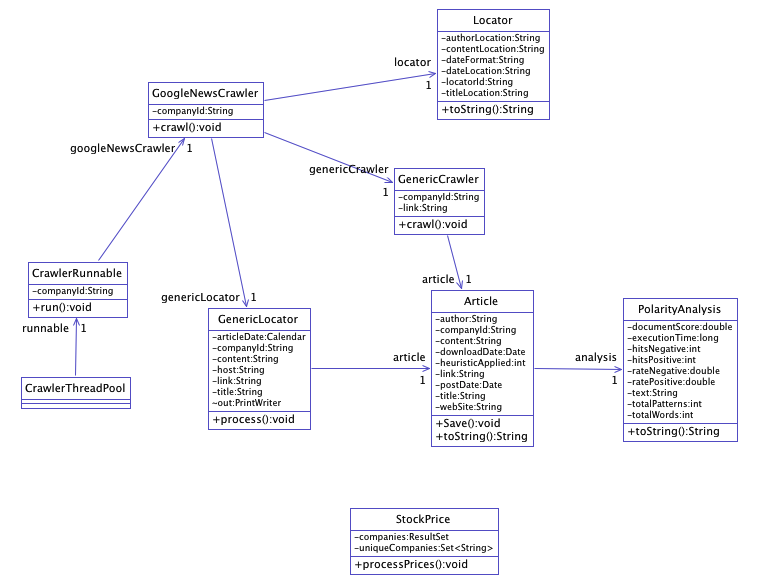
\includegraphics[scale=0.55]{ClassDiagram}
		\caption{Class diagram of the framework.}\label{fig:ClassDiagram}
	\end{figure}

\section{Configuration Files}

Because of the nature of the thesis, it is suitable to manage configuration files in order to change the behaviour of the framework without changing a single line of code, and of course not to \emph{hardcode} text or any string inside the code. The framework consists on 10 configuration files that contains around 40 different variables that can be set. We will describe each of them.

\begin{itemize}
	\item \emph{main.properties}\label{main.properties}: This configuration file was conceived for the user not to input 9 different parameters when he will run the application on the console. It contains only the paths for the other configuration files. We will introduce the required format, it is not necessary that the files have a strict name. What is mandatory is not to change the name of the variables (in the left).
	
\begin{lstlisting}
genericConstantsProperties = /Path/constants.properties
crawlerProperties = /Path/crawler.properties
databaseProperties = /Path/database.properties
dateFormatProperties = /Path/dateFormat.properties
filesProperties = /Path/files.properties
googleNewsProperties = /Path/googleNews.properties
jsoupProperties = /Path/jsoup.properties
locatorsProperties = /Path/locators.properties
priceProperties = /Path/priceEndPoint.properties
\end{lstlisting}
	
	\item \emph{constants.properties}:  This file is simple but important as well. Because here we define the debug mode of the application; and it defines the amount of output in console, if we will use the generic locator and if we will save the article or if it will be in simulation mode.
	
\begin{lstlisting}
DEBUG = true
USE_GENERIC_LOCATOR = true
SAVE_ARTICLE = true
\end{lstlisting}
	
	\item \emph{crawler.properties}\label{crawlerProperties}: This property file is the most important one for the crawler, because here we define for each host where exactly is the title, date, content and author of one particular article. For example; for the host \url{www.financialexpress.com} after following the procedure explained in \ref{locators}

\begin{lstlisting}
GenericCrawler.source.1 = www.fool.com;h1.xlHeader;div.entry-content;span[itemprop=author]; span.dateline;MMMM dd, yyyy
GenericCrawler.source.11 = www.financialexpress.com;h1;font;div.dateline;div.dateline;MMM dd yyyy
GenericCrawler.source.13 = indiatoday.intoday.in;h1;div.strleft;div.strstrap;div.strstrap;MMMM dd, yyyy
\end{lstlisting}	

	\item \emph{database.properties}: In this file, we will define the connection parameters of the database; host, user name, password, database name, port, and connection string (which is a formatted string, and it would look like:  \url{jdbc:mysql://localhost:port/DiplomaWork?user=myUser&password=myPassword})

\begin{lstlisting}
DB_HOST = localhost
DB_USER_NAME = myUser
DB_PASSWORD = myPassword
DB_NAME = DiplomaWork
DB_PORT = 8889
DB_CONNECTION_STRING = jdbc:mysql://%s:%s/%s?user=%s&password=%s
\end{lstlisting}

	\item \emph{dateFormat.properties}: In this file we define the possible date formats that we can find in the different Web pages. If we find more date formats in any other Web page, we just add a new row in this file with the regular expression of the desired date format.
	
\begin{lstlisting}
date.regex.1 = ([0-9]{4}-[0-9]{1,2}-[0-9]{1,2})
date.regex.2 = ([0-9]{1,2}(-|/)[0-9]{1,2}(-|/)[0-9]{2,4})
\end{lstlisting}

	\item \emph{files.properties}: Here we define a list of several files for several purposes. Here we define where the GATE home folder is, the Plugin folder, the JAPE grammar file, and the \emph{bag of words} (positive, negative and stop words)

\begin{lstlisting}
GATE_HOME_FOLDER = /Applications/GATE_Developer_7.1
GATE_PLUGIN_FOLDER = /plugins
GATE_JAPE_FILE = /files/patterns.jape
WORD_BANK_NEGATIVE = /files/negative-words.txt
WORD_BANK_POSITIVE = /files/positive-words.txt
WORD_BANK_STOP = /files/stop-words.txt
\end{lstlisting}

	\item \emph{stocks.properties}\label{stocks.properties}: This File contains the code of the stocks that will be crawled in the framework. We show here only a small part of the file. 
	
\begin{lstlisting}
company.1 = MMM
company.2 = AXP
company.3 = T
company.4 = BA
company.5 = CAT
company.6 = CVX
company.7 = CSCO
company.8 = KO
company.9 = DD
company.10 = XOM
\end{lstlisting}

	\item \emph{googleNews.properties}: To explain this file we will refer to the Locators (\ref{locators}), where we explain how to get the articles from google news. And here, we define the parameters (If we observe in detail the figures: \ref{fig:News_001}, \ref{fig:News_002}, \ref{fig:News_003}, \ref{fig:News_004}  we can see the name/id from the tag that contains every piece of information) how to do it; the url of the news end point, the location in the Web page of the main container, title, link, date. 
	
\begin{lstlisting}
GOOGLE_NEWS_END_POINT = https://www.google.com/finance/company_news?q=%s&start=%s&num=%s
GOOGLE_NEWS_RESULTS_PER_PAGE = 50
GOOGLE_NEWS_CONTAINER = div#news-main
GOOGLE_NEWS_ROW_ID = div.g-section.news.sfe-break-bottom-16
GOOGLE_NEWS_ROW_TITLE_ID = n-cn-
GOOGLE_NEWS_ROW_SOURCE = src
GOOGLE_NEWS_ROW_DATE = date
\end{lstlisting}	
	
	\item \emph{jsoup.properties}: In this work we help ourselves with and HTML parser called \emph{JSOUP}, and we have to set up some parameters in this configuration file, in order not to \emph{hardcode} strings in the source code, as previously mentioned. We define here, the name of the user agent, the url where we are supposed to be referred, if we should ignore the http errors or not, and the time out in order to not to wait so long if some news article host is offline.
	
\begin{lstlisting}
JSOUP_USER_AGENT = Mozilla/5.0 (Windows U WindowsNT 5.1 en-US rv1.8.1.6) Gecko/20070725 Firefox/2.0.0.6
JSOUP_REFERAL_URL = http://www.margaritka.com
JSOUP_IGNORE_HTTP_ERRORS = true
JSOUP_HTTP_SUCCESS_CODE = 200
JSOUP_TIME_OUT = 30000
\end{lstlisting}
	
	\item \emph{locator.properties}: Here, for this property file we will refer as well to the Locators (\ref{locators}) and to the crawler.properties file (\ref{crawlerProperties}). Because, in this file we define how many lines of comment the \emph{crawler.properties} has, what is the element that divides one particular locator in order to make one tag unique or to search in the HTML document for one specific tag. We define as well, what will be the minimum size of the article in order for the Generic Locator (\ref{genericLocator}) to extract it and process it.
	
\begin{lstlisting}
LOCATOR_HEADER_LINES_COUNT = 3
LOCATOR_ELEMENT_DIVIDER = ->
LOCATOR_MIN_ARTICLE_SIZE = 200
\end{lstlisting}
	
	\item \emph{priceEndPoint.properties}: In this file, we defined the URL of the price endpoint that we will describe later in the section: {priceRetrieval}, This is a formatted string in which we will be inputing the code of company, the start and also end date; our start date for all the companies will be on January 1st, 2012. This would be a bit inefficient because we would be downloading prices/data that we won't need, but in this case this details are ignored because of the small size of the file that we are downloading (approximately 30 - 50 KB). If we would like to change this date, we should just modify this file.

\begin{lstlisting}
PRICE_END_POINT = http://ichart.finance.yahoo.com/table.csv? s=%s&a=%d&b=%d&c=%d&d=%d&e=%d&f=%d&g=d&ignore=.csv
FIRST_DAY = 1
FIRST_MONTH = 1
FIRST_YEAR = 2012
\end{lstlisting}
	
\end{itemize}

\section{Singleton}

In our framework we will use the pattern that in software engineering is called \emph{Singleton} and to define it we will rely on the work of  Johnson \cite{S2014}, which according to the source is: \emph{a design pattern that restricts the instantiation of a class to one object. This is useful when exactly one object is needed to coordinate actions across the system. The concept is sometimes generalized to systems that operate more efficiently when only one object exists, or that restrict the instantiation to a certain number of objects. The term comes from the mathematical concept of a singleton.}

The reason of the \emph{Singleton} is simple but it has a huge impact in the performance of the application. Because it would be non sense to load all libraries, classes, database drivers, database connection and bag of words for every article that we would be analysing. The application takes around 10 seconds to start; but we should see this ten seconds as an investment, because as we mention we will spend them only once in the startup of the application. The pseudocode is presented in the Algorithm \ref{singletonAlgorithm}, and the part that takes more time is initialising the GATE text mining framework; this framework is presented in the \emph{Part-of-Speech} (\ref{partOfSpeech}). If we will be loading the class for first time, the \emph{unique\_instance = NULL}, so we will load the necessary information, otherwise we will not do anything because the class, frameworks and libraries will be already loaded in memory. The implementation of the class is in the file: \emph{\ul{Singleton.java}}

\begin{algorithm}
\caption{Singleton algorithm}\label{singletonAlgorithm}
\begin{algorithmic}[1]

\IF{$unique\_instance = NULL$}
		\STATE Load the \emph{bag of words};
		\STATE Load the \emph{database drivers};
		\STATE Initialise \emph{GATE Framework};
\ENDIF
\end{algorithmic}
\end{algorithm}

\section{Generic Objects}

In this section, we will describe the generic object and classes that doesn't have to do directly with the implementation of the \emph{News Crawler} and \emph{Sentiment Analysis}.

\begin{itemize}
	\item \emph{\ul{PriceDetail.java}}: We will be using this class in order to parse every day prices for a particular company.
	\item \emph{\ul{Utilities.java}}: This class as it names suggest, contain only utility functions/methods; all of them are public and static; it means that this class doesn't need to be instantiated in order to access its methods. Some of the methods that can be found here are: counting lines from a text file, count occurrences of a word in a text, count words in a text, simple debug methods, extract date from text, correlation, extract querystring parameters from a URL, download web document, logarithm base \emph{2}, logarithm base \emph{n}, implementation of a \emph{NEAR} method, parse and select HTML, memory information, check if a link exists, among others.
\end{itemize}

\section{News Crawler}

This class is one of the two more important, because here we will be implementing the Crawler that will be downloading and extracting the desired information from web pages. As explained earlier, in the section \ref{webCrawler}, we will be relying on the \emph{google news endpoint}, which previously has been analysed in order to get to know its structure. The decision of crawling the \emph{Google News endpoint} is because the information is already segmented by category (Because we will only be needing financial news) and company, as well here we have news articles from different providers, and they don't provide (or is not know) a public API to retrieve this information. Sometimes, only a particular provider provides some sort of \emph{pseudo-API} (RSS feeds, usually).

\begin{itemize}
	\item \emph{\ul{GoogleNewsCrawler.java}}\label{GoogleNewsCrawler}: This class is the starting point of the process, where the input data is the code of the company in the stock market. After the instantiation of the class, we will immediately start crawling the page. After this, we will be generating dynamically a link starting from zero (0) to the article number \emph{N}, with offsets of \emph{GOOGLE\_NEWS\_RESULTS\_PER\_PAGE} (50 by default). After this we will download the Web page, and we will be repeating this process until the \emph{stop condition} is fulfil; which is a big change in the HTML structure of the Web page. The process that we will be repeating besides the link generation, will be the link extraction from the already generated link; which contains the article title, date and link; but this process will be in charge of \emph{\ul{GenericCrawler.java}}.
	\item \emph{\ul{GenericCrawler.java}}: This class is in charge of every of the extracted links, and in order to work it will need two parameters; the companyId and extracted link. After this we will download the webpage and according to the \emph{Locator} or \emph{Generic Locator} we will be extracting the article title, date and link, with a high accuracy.	
	\item \emph{\ul{Locator.java}}: This class is used in the \emph{Generic Crawler} and is used in the \emph{Singleton} class in order to create an array with the information in \emph{crawler.properties}. Basically this class is a container in order to extract from the HTML structure the data of our interest.
	\item \emph{\ul{GenericLocator.java}}: This class maybe has a similar name as the previous one, but even if they aim the same objective, which is to extract data from the news article; this class implement a simple heuristic in order to try to get the data from the news article without the implementation of a \emph{Locator} as mentioned in the section \ref{genericLocator} with its respective algorithm (algorithm \ref{genericLocatorAlgorithm}).
	\item \emph{\ul{Article.java}}: This class is the integration point between the \emph{News Crawler, Sentiment Analysis} and the  \emph{Database}. Basically after an article is successfully parsed in the \emph{News Crawler}, an \emph{Article} object is created and the \emph{Polarity Analysis} class is instantiated inside this class, and finally, after every process is finished the news article is saved. 
\end{itemize}

\section{Sentiment Analysis}

Here, we will be describing the implementation of the theory described in the section \ref{sentimentAnalysis} and its respective algorithm ({unsupervisedAlgorithm}).

The implementation is in the file: \emph{\ul{PolarityAnalysis.java}}; and it needs only some text as a parameter; here we will remove the stop words and "weird" characters that we could found in the text and we will count the number of positive and negative words founded in the text according to our \emph{bag of words}, and of course, we will count the total number of words. After this, we will use the API of GATE (section: \ref{gate}) in order to extract automatically the words that fulfils the conditions presented early in the table \ref{tab:twoWordPhrases}; as presented in the example in the section \ref{partOfSpeech}, and for each pair of words that fulfil this conditions we will apply the operator \emph{NEAR} in order to take the ten left and rightmost words from the pattern found that fulfil the conditions of the table \ref{tab:twoWordPhrases}. After this, we will calculate the semantic orientation of each phrase found, we will calculate the average and some other useful statistics like: total number of patterns, rate of positive and negative words, execution time, etc. As output the class will return the \emph{score of the document}.

\section{Parallel algorithm implementation}\label{parallelImplementation}

\emph{\ul{CrawlerThreadPool.java}}: In this class is implemented the algorithm \ref{parallelCrawlerAlgorithm} defined in the chapter \ref{analysisDesign}. This is the starting point of the framework. The class expects as an argument the path to the main configuration file, where every other configuration is stored. (As mentioned earlier in the section: \ref{main.properties}), then the class calculates how many threads the framework will be using. Then for every company defined in stocks.properties (see \ref{stocks.properties}) an object of type GoogleCrawlerNews is created (see \ref{GoogleNewsCrawler}); which represent the sequential solution, after this, the framework waits until the last thread finish its execution, finally, the stock prices are gathered and the information is summarised as described in the section \ref{priceRetrieval}. An evaluation of the performance of the parallel solution will be described in the chapter \ref{experimentalEvaluation}.
 
\section{Price retrieval \& Summarization}\label{priceRetrieval}

\emph{\ul{StockPrice.java}}: This class firstly performs a summarisation of the data; in order to generate a table which will contain calculated data and general daily statistics about the companies (price, delta, number and percentage of positive and negative articles, etc.) which a posteriori will be correlated in order to present final results faster.

To retrieve the price we will use \url{finance.yahoo.com}, because it has a Web API which will allow us to access the stock price data in an easy way. We will find in the file: "priceEndPoint.properties" the link of the news endpoint in which we will define basic parameters like: start date and end date.
\\\\
\url{http://ichart.finance.yahoo.com/table.csv} 
\\\\
It is worth to mention that we will consider the close price of the stock. And to get this price we will download the "csv" file, which contains several fields: Date, Open, High, Low, Close, Volume, Adj Close*. In our case we will only need the "Close" field. Unfortunately; until today, there is no way to make a request asking only for the specific field we need, and make the transmission of the file lighter.

First of all, we will count the articles (positive, negative, total) per day, and for that we will be calling a \emph{Stored Procedure} in the database, which for simplicity every time that it is executed will delete all registries from the table, and it will perform calculations per every day were exists news articles, the output data (Ids of the companies) of the \emph{Stored Procedure} will be used to download the prices. 

After this, for each company returned in the output, we will download the prices file and we will parse the mentioned file. Once the data is parsed, we will be saving in the database the final prices.

\section{Startup}

When we are talking about the startup of the application, basically is the class that contains the \emph{main} method; and in our case there are several files, and most of them have been used in the development phase; to test individual parts of the framework. The one class that must be invoked in order to collect the data is \emph{CrawlerThreadPool.java}.

\begin{itemize}
	\item \emph{\ul{CrawlerThreadPool.java}}: As we mention before this is the class that startup the framework. But it has a particularity, instead of the sequential implementation of the framework, this class implements multi-threading in the application, which \emph{speedup} the application considerably; we will verify this fact in the experimental section (\ref{experimentalEvaluation}).
	\item \emph{\ul{CrawlerRunnable.java}}: This is the implementation of a \emph{Runnable} interface for our own purposes, which initialise the \emph{News Crawler} for a particular company.
	\item \emph{\ul{PolarityAnalysisTester.java}}: This class is a tester which help us to estimate the polarity of a particular text.
	\item \emph{\ul{GenericLocatorTester.java}}: For a Web page that has no locator defined, this class implement a tester of the \emph{Generic Locator} to extract the information of our interest.
	\item \emph{\ul{PriceTester.java}}: This class implements a main function for the summarisation class \emph{StockPrice.java}.
	\item \emph{\ul{ProcessLinksThreadPool.java}}: This class extracts from the database non-parsed links and try to parse them using the \emph{Generic Locator}.
	\item \emph{\ul{ProcessLinksRunnable.java}}: This is the implementation of a \emph{Runnable} interface for our own purposes, which initialise the \emph{Generic Locator} class.
\end{itemize}


\section{Database}

The database, as we mention earlier in the section \ref{pageRepository}, it will be our \emph{page repository}, and the place where we will keep statistics and the companies that we will be crawling. The entity-relation model was designed in \emph{MySQLWorkbench}; which is an open source visual database design tool. 

The model is quite simple, it consists on seven tables that we will be discussing here. The entity-relation model is shown on the figure \ref{fig:DB_001}.

	\begin{figure}\centering
		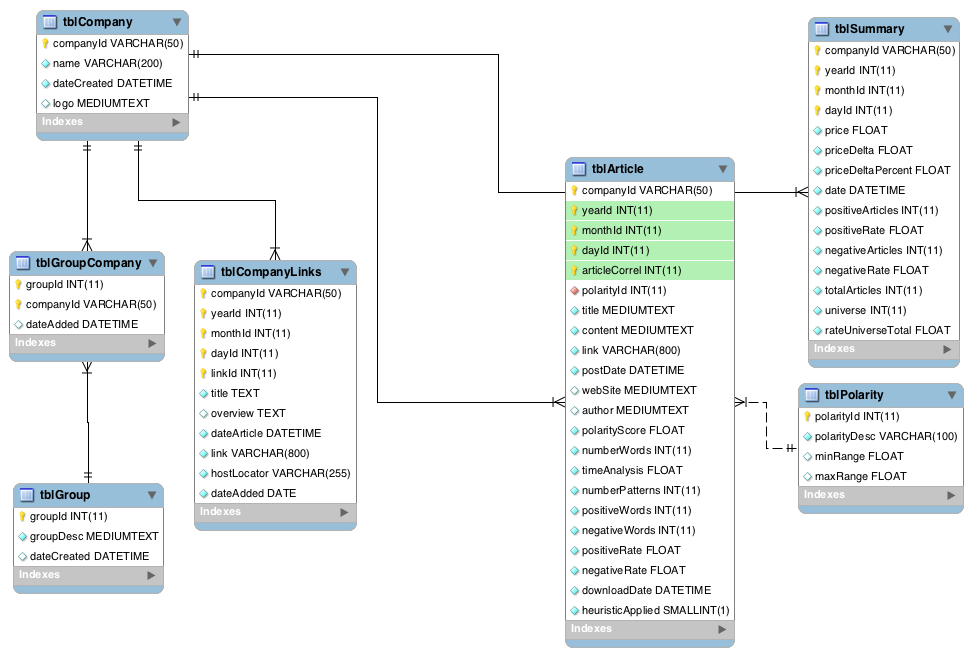
\includegraphics[scale=0.45]{DB_001}
		\caption{Entity-relation diagram of the database.}\label{fig:DB_001}
	\end{figure}

\begin{itemize}
	\item \emph{tblGroup}: We will be storing here the name of one particular group that will contain several companies; this with the objective to consolidate stocks in one particular group, following the idea for example of the industrial average \emph{Dow Jones} which tracks the 30 largest U.S. companies., \emph{NASDAQ} which has several companies that are in \emph{Dow Jones} as well.
	\item \emph{tblGroupCompany}: This entity is related directly with \emph{tblGroup} because companies and groups will be joining here. Here we will define which company belongs to which group. This table represents one \emph{many to many} relation. 
	\item \emph{tblCompany}: This entity basically defines a company, with its code, name and logo.
	\item \emph{tblCompanyLinks}: This entity is a repository of links, if a link goes through the framework, it will be saved here; doesn't matter if it is parsed or not. The parsed links will be in \emph{tblArticle}.
	\item \emph{tblArticle}: Here relies most of the information that we will be using for summarisation and experimentation. We identify an article by company, date of publication, and a correlative. And in this entity we will be storing the direction of the polarity, title, content of the article, author, link, score, website, execution time, if heuristic was applied to the link, among others. 
	\item \emph{tblPolarity}: It is a catalog that defines when an article will be positive or negative, with the ranges defined in every tuple.
	\item \emph{tblSummary}: As we know, a company can have several or maybe hundreds of articles per day. And to create a query that would compute this information is would be quite complex, time consuming and probably messy as well. The objective of this table is to summarise per company and per day the previously collected data: price, delta and delta percent of the stock and number of positive and negative articles collected.
\end{itemize}

Another feature of the database engine used in the framework are the \emph{Stored procedures} and \emph{functions}. And each of the stored procedures used are described here. As a naming convention the \emph{function} names starts with \emph{fn\_} and the  \emph{Stored procedure} names starts with \emph{pr\_}.

\begin{itemize}
	\item \emph{fn\_calculate\_price\_delta}: This function calculates the change (delta) in price of a particular stock from the current day with the previous working day.
	\item \emph{fn\_previous\_working\_day}: This function calculates the previous working day and the result is used by the function \emph{fn\_calculate\_price\_delta} in order to calculate the delta of the price.
	\item \emph{pr\_add\_article}: This stored procedure saves one article to the database, and outputs the correlative of the article generated.
	\item \emph{pr\_init\_database}: This stored procedure initialise the database, we only need to populate the table \emph{tblPolarity}.
	\item \emph{pr\_link\_exist}: Check if a link is already saved in the database; if not it saves it.
	\item \emph{pr\_summarize}: This stored procedure populates the table \emph{tblSummary} daily, with the respective information (Number of positive and negative articles).
	\item \emph{pr\_update\_summary}: This stored procedure is started after the summarisation (\emph{pr\_summarize}). After we download the prices, as we mention in the section \ref{priceRetrieval}, and what this procedure does is to update one particular row and calculating the delta of the stock price for that particular day.
\end{itemize}

\section{Libraries}
We will describe briefly the libraries used for the implementation of the framework. 

\begin{itemize}
	\item \emph{GATE}\label{gate}: According to Miner, Elder, Fast, Hill, Nisbet and Delen in his book \emph{Practical Text Mining and Statistical Analysis for Non-structured Text Data Applications} \cite{G2014}, \emph{GATE} stands for General Architecture for Text Engineering, which is described as an the leading Open Source tool kit for text mining. Which was written in Java and its tools were originally developed at the University of Sheffield in beginning of 1995 and now is used worldwide by a wide community of scientists, companies, teachers and students for all sorts of natural language processing tasks, including information extraction in many languages. 
	
	In our work, we have used \emph{GATE} as text pattern extraction; We have mention a practical example in the section {partOfSpeech} using the \emph{GATE} user interface, and in the framework this same example is implemented in code through the \emph{GATE API}.
	
	\item \emph{JSOUP}: is an HTML parser, its “jquery-like” and “regex” selector syntax is very easy to use and flexible enough to get extract any particular information from a Web page. It implements the WHATWG HTML5 specification, and parses HTML to the same DOM as modern browsers do.
	
	In our work, we have used \emph{JSOUP} as HTML parser, in order to download and extract specific data from a Web page that doesn't provide a Web API. Our work is not the kind of work that is written in stone, because we have to be conscious that any change on the structure of the page that we are parsing, we must change the details to specify where the data that we want is located.
	 
\end{itemize}


	
	\chapter{Experimental evaluation \& Results}\label{experimentalEvaluation}
	
		In this section we will be demonstrating the experimental evaluation of the Sentiment Analysis algorithm we have implemented; which is a crucial part of our framework, and we will have a look on at the execution time of the whole framework. In addition to this we will be showing the results that we obtain while collecting the data; the considered data collection period was: \emph{April 1st, 2014 - April 30th, 2014}. We have to have in mind that we will be considering only working days from \emph{Monday - Friday}; and if it was some holiday in this period, it was not considered in the analysis because the \gls{NYSE} is close in this period.

\section{Experimental evaluation.}

In this section we will be showing the behavior of the framework in it's most important and CPU time consuming part: \emph{The Polarity Analysis}; as shown in the section \ref{sentimentAnalysis}. In addition to the experimental evaluation, we have implemented \emph{multi-threading} in our framework, and we will be demonstrating experimentally how it \emph{speedup} the framework.

We will be using the \emph{Linear least squares} to get experimentally the complexity of the algorithm. \emph{Linear least squares \cite{L2014} is an approach fitting a mathematical or statistical model to data in cases where the idealized value provided by the model for any data point is expressed linearly in terms of the unknown parameters of the model. The resulting fitted model can be used to summarize the data, to predict unobserved values from the same system, and to understand the mechanisms that may underlie the system.}

We are presenting the results of this particular section in the table \ref{tab:wordsTime} and graphically in the figure \ref{fig:wordsTime} and even if the \emph{Linear least squares} (figure \ref{fig:Experiment_001}) method suggest a degree four complexity according to the data, we will take the complexity in degree 3, because of the amount of nested loops in the code (3). The equation that fits the better has the following form: 
\[4.98946x10^-7 x^3-0.00239705 x^2+4.28487 x-422.422\] 
which asymptotically is equivalent on average to 
\[\theta(n^3)\] 
We can verify the details of the \emph{Linear least squares} method in the following link:
\\\\
\url{http://www.wolframalpha.com/input/?i=fit+%2814%2C+229.7524129%29%2C%281014%2C+803.3164669%29%2C%282014%2C+1601.227397%29%2C%283014%2C+2921.279661%29%2C%284014%2C+3171.105263%29%2C%285014%2C+5282.681818%29%2C%286014%2C+3400.888889%29%2C%287014%2C+9654.75%29%2C%288014%2C+11768.33333%29%2C%289014+%2C+4507.2%29}

\begin{figure}\centering
	\caption{Number of words vs. Execution time (ms)}\label{fig:wordsTime}
	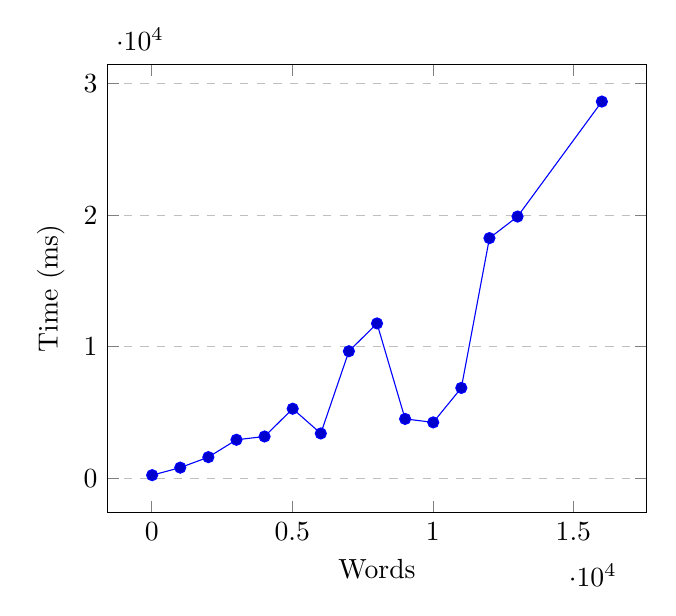
\begin{tikzpicture}
		\begin{axis}[ 
			xlabel=Words,
			ylabel=Time (ms),
			ymajorgrids=true,
			grid style=dashed,
  				]	 
			\addplot coordinates {
				(14, 229.7524129)
				(1014, 803.3164669)
				(2014, 1601.227397)
				(3014, 2921.279661)
				(4014, 3171.105263)
				(5014, 5282.681818)
				(6014, 3400.888889)
				(7014, 9654.75)
				(8014, 11768.33333)
				(9014 , 4507.2)
				(10014, 4242.875)
				(11014, 6866)
				(12014, 18255)
				(13014, 19895)
				(16014, 28639.5)
				};
		\end{axis}
	\end{tikzpicture}
\end{figure}

\begin{table}\centering
	\caption{Number of words vs. Execution time (ms)}\label{tab:wordsTime}
   	\begin{tabular}{ | p{4cm\textwidth} | p{4cm\textwidth} |}
   	\hline

\textbf{Number of Words}  & \textbf{Average Execution time (ms)}       \\\hline
14-1013     & 229.7524129 \\\hline
1014-2013   & 803.3164669 \\\hline
2014-3013   & 1601.227397 \\\hline
3014-4013   & 2921.279661 \\\hline
4014-5013   & 3171.105263 \\\hline
5014-6013   & 5282.681818 \\\hline
6014-7013   & 3400.888889 \\\hline
7014-8013   & 9654.75     \\\hline
8014-9013   & 11768.33333 \\\hline
9014-10013  & 4507.2      \\\hline
10014-11013 & 4242.875    \\\hline
11014-12013 & 6866        \\\hline
12014-13013 & 18255       \\\hline
13014-14013 & 19895       \\\hline
16014-17013 & 28639.5    \\\hline

    \end{tabular}
\end{table}

\begin{figure}\centering
	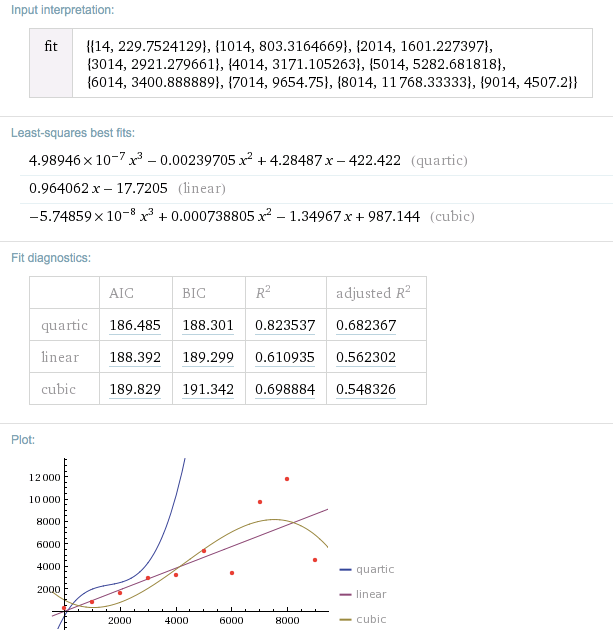
\includegraphics[scale=0.65]{Experiment_001}
	\caption{Least-squares Analysis - Words}\label{fig:Experiment_001}
\end{figure}


We are presenting the results of this particular section in the table \ref{tab:patternTime} and graphically in the figure \ref{fig:patternTime}. In the case of the patterns, this is strongly related to the complexity of the algorithm, because number of patterns will define how many loops will be executing; again, we perform the \emph{Linear least squares} method, in order to figure out the average time complexity of the algorithm. We will accept the linear equation, and it look as follows:
\[23.3226 x-2619.46\] 
which asymptotically is equivalent on average to 
\[\theta(n)\] 
We can verify the details of the \emph{Linear least squares} method in the following link:	
\\\\	
\url{http://www.wolframalpha.com/input/?i=fit+%2899+%2C+286.5746529+%29%2C%28199%2C+1430.8487+%29%2C%28299%2C+3201.441441+%29%2C%28399%2C+5272.302326+%29%2C%28499%2C+6610.857143+%29%2C%28599%2C+15193.8+%29%2C%28699%2C+21042.5+%29%2C%28799%2C+11245+%29%2C%28899%2C+15079+%29%2C%28999%2C+25786.33333+%29%2C%281099%2C+19710%29}

\begin{figure}\centering
	\caption{Number of patterns vs. Average execution time (ms)}\label{fig:patternTime}
	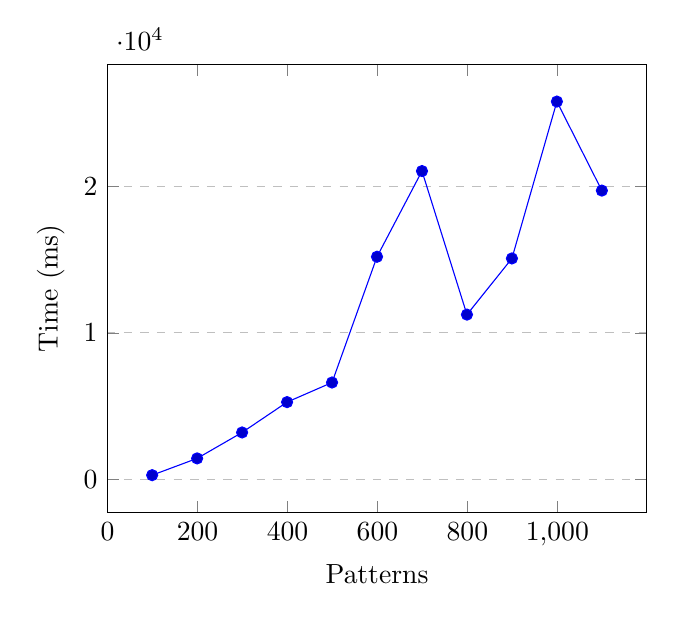
\begin{tikzpicture}
		\begin{axis}[ 
			xlabel=Patterns,
			ylabel=Time (ms),
			ymajorgrids=true,
			grid style=dashed,
  				]	 
			\addplot coordinates {
(99       , 286.5746529 )
(199    , 1430.8487   )
(299    , 3201.441441 )
(399    , 5272.302326 )
(499    , 6610.857143 )
(599    , 15193.8     )
(699    , 21042.5     )
(799    , 11245       )
(899    , 15079       )
(999    , 25786.33333 )
(1099  , 19710      )
				};
		\end{axis}
	\end{tikzpicture}
\end{figure}


\begin{table}\centering
	\caption{Number of patterns vs. Average execution time (ms)}\label{tab:patternTime}
   	\begin{tabular}{ | p{4cm\textwidth} | p{4cm\textwidth} |}
   	\hline
\textbf{Number of Patterns}  & \textbf{Average Execution time}       \\\hline
0-99       & 286.5746529 \\\hline
100-199    & 1430.8487   \\\hline
200-299    & 3201.441441 \\\hline
300-399    & 5272.302326 \\\hline
400-499    & 6610.857143 \\\hline
500-599    & 15193.8     \\\hline
600-699    & 21042.5     \\\hline
700-799    & 11245       \\\hline
800-899    & 15079       \\\hline
900-999    & 25786.33333 \\\hline
1000-1099  & 19710      \\\hline

    \end{tabular}
\end{table}

\begin{figure}\centering
	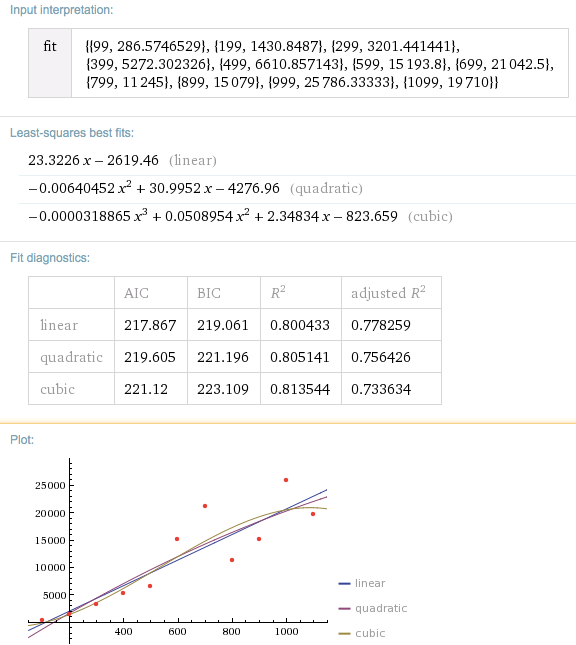
\includegraphics[scale=0.65]{Experiment_002}
	\caption{Least-squares Analysis - Patterns}\label{fig:Experiment_002}
\end{figure}


\subsection{Multi-Threading Performance}

We are presenting the results of this particular section in the table \ref{tab:threadsTime} and graphically in the figures: \ref{fig:threadsTime}. For this part we will cite professor Tvrdík \cite[p. 3-9]{T2011} in the chapter \emph{Performance and Scalability of parallel algorithms.}, where there are some metrics in order to measure the performance of parallel algorithms. We will describe several of this metrics in order to analyze the parallelism of our framework.

\begin{itemize}
	\item \emph{Parallel time T(n,p)}: Is the time elapsed from the beginning of a p-processor (In our case we will consider software threads) parallel algorithm solving a problem instance of size \emph{n} until the last processor finishes the execution. \emph{T(n,p)} is obtained by \emph{counting} or by \emph{measuring the total time complexity} of:
	\begin{itemize}
		\item \emph{parallel computationl} steps. e.g., arithmetic operations.
		\item \emph{parallel communication} steps. i.e., transfers and exchanges of data between processors.
	\end{itemize}	
	Due to the second component \emph{T(n,p)} depends on the architecture of a parallel computer. Therefore the performance evaluation of a parallel algorithm must \emph{always} consider the architecture. In a specific algorithm, \emph{p} is always chosen as a suitable function of \emph{n}.

	\item \emph{Parallel Speedup S(n,p)}: If both, sequential and parallel algorithm with \emph{p} processors are executed under the same conditions, the best speedup we can hope is for \emph{p}. Due to the communication overhead, such a speedup is achievable only if the solution of the problem contains enough parallelism, the communication part is negligible, and all the processors perform only useful computation under ideal load balancing and synchronization. In practice, a linear speedup \emph{kp} for some constant 0 < k <1 is quite satisfactory.
	
	\item \emph{Parallel cost C(n,p)}: 
	\[C(n,p) = p * T(n,p) \] 
	This metric is a bit coarse-grained. It is actually an upper estimate of the operational complexity. It gives the total number of operations as if all processors were active since the beginning till the end (like the slowest processor). But this is what parallel systems with job schedulers typically allow: prior to a parallel computation, a user job is assigned p processors and these are released only after the whole parallel computation has finished. In such systems, \emph{C(n,p)} is a useful metric, since idling processors or processors that finished their subtasks faster are useless for the other users until the whole computation finishes. Since any parallel algorithm can be trivially simulated on a uniprocessor machine with multiprogramming, we get that \emph{The parallel Cost, cannot be less than the complexity of the best sequential algorithm:}
	\[C(n,p) = \Omega(SU(n)) \] 
	\emph{In the best case, the cost is of the same order as the sequential complexity:}
	\[C(n,p) = O(SU(n)) \] 
	
	\item \emph{Parallel Efficiency E(n,p)}
	\[E(n,p) = \frac{SU(n)}{C(n,p)} = \frac{S(n,p) * T(n,p)}{p * T(n,p)} =  \frac{S(n,p)}{p} \leq 1 \] 
	Basically, the Parallel efficiency is the speedup per processor.
\end{itemize}

Now, that we prepare a theoretical background, we will be mentioning the characteristics of the hardware where the tests have been performed, and after this we will be introducing the experimental results, which are shown in the table \ref{tab:threadsTime}.

\begin{itemize}
	\item CPU: 1.86 GHz Intel Core 2 Duo
	\item Memory:  4 GB, 1067 MHz DDR3
	\item Operative System: OS X 10.8.5 (12F45)
	\item Hard drive: APPLE SSD TS128C Media
	\item Considered size of the problem: \emph{n=35}
\end{itemize}

\begin{table}\centering
	\caption{Multi-Threading Performance Analysis}\label{tab:threadsTime}
   	\begin{tabular}{ | p{2.5cm\textwidth} | p{2.5cm\textwidth} | p{2.5cm\textwidth} | p{2.5cm\textwidth} | p{2.5cm\textwidth} |}
   	\hline
\textbf{Number of threads} & \textbf{Execution time (s) T(n,p)}& \textbf{Speedup S(n,p)} & \textbf{Efficiency E(n,p)} & \textbf{Cost C(n,p)} \\\hline
1               & 223.816 	&	 1			&	1			&	223.816          \\\hline
2               & 124.441	&	 1.79857121	&	0.899285605	&	248.882           \\\hline
3               & 103.705	&	 2.158198737 	&	0.719399579	&	311.115           \\\hline
4               & 111.66	&	 2.004442056	&	0.501110514	&	446.64            \\\hline
5               & 101.099	&	 2.213830008	&	0.442766002	&	505.495           \\\hline
6               & 100.934	&	 2.217449026	&	0.369574838	&	605.604           \\\hline
7               & 95.115	&	 2.353109394 	&	0.336158485	&	665.805            \\\hline
8               & 89.632	&	 2.497054623	&	0.312131828	&	717.056            \\\hline
9               & 91.493	&	 2.446263649	&	0.271807072	&	823.437            \\\hline
10              & 93.347	&	 2.397677483	&	0.239767748	&	933.47            \\\hline
11              & 124.689	&	 1.794993945	&	0.163181268	&	1371.579           \\\hline
12              & 131.235	&	 1.705459672	&	0.142121639	&	1574.82           \\\hline
13              & 134.524	&	 1.6637626	&	0.127981738	&    1748.812      \\\hline

    \end{tabular}
\end{table}

Now that we have the execution data, we will visualize each of them in a plot. \emph{Time complexity T(n,p)} can be visualized in the figure \ref{fig:threadsTime}, \emph{Cost C(n,p)} in the figure \ref{fig:threadsCost}, \emph{Speedup S(n,p)} in the figure \ref{fig:threadsSpeedup}, and the \emph{Efficiency E(n,p)} in the figure {fig:threadsEfficiency}.

\begin{figure}\centering
	\caption{Number of threads vs Average execution time (s)}\label{fig:threadsTime}
	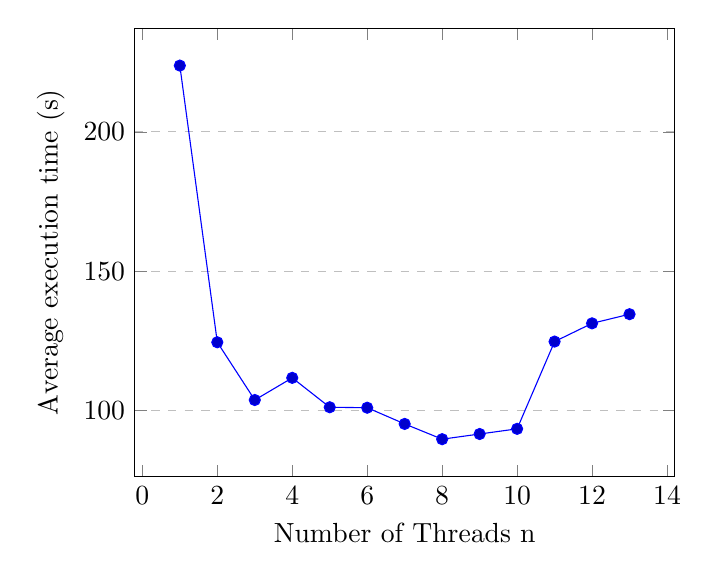
\begin{tikzpicture}
		\begin{axis}[ 
			xlabel=Number of Threads n,
			ylabel=Average execution time (s),
			ymajorgrids=true,
			grid style=dashed,
  				]	 
			\addplot coordinates {
(1               , 223.816           )
(2               , 124.441           )
(3               , 103.705           )
(4               , 111.66            )
(5               , 101.099           )
(6               , 100.934           )
(7               , 95.115            )
(8               , 89.632            )
(9               , 91.493            )
(10              , 93.347            )
(11              , 124.689           )
(12              , 131.235           )
(13              , 134.524          )
				};
		\end{axis}
	\end{tikzpicture}
\end{figure}

\begin{figure}\centering
	\caption{Number of threads vs Cost}\label{fig:threadsCost}
	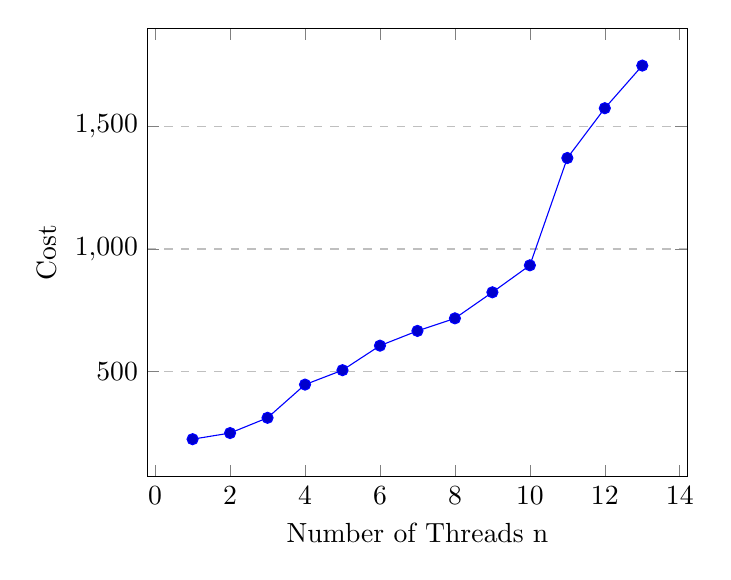
\begin{tikzpicture}
		\begin{axis}[ 
			xlabel=Number of Threads n,
			ylabel=Cost,
			ymajorgrids=true,
			grid style=dashed,
  				]	 
			\addplot coordinates {
(1               , 223.816            )
(2               , 248.882            )
(3               , 311.115           )
(4               , 446.64            )
(5               , 505.495          )
(6               , 605.604           )
(7               , 665.805            )
(8               , 717.056            )
(9               , 823.437          )
(10              , 933.47            )
(11              , 1371.579           )
(12              , 1574.82         )
(13              , 1748.812          )
				};
		\end{axis}
	\end{tikzpicture}
\end{figure}

\begin{figure}\centering
	\caption{Number of threads vs Speed up}\label{fig:threadsSpeedup}
	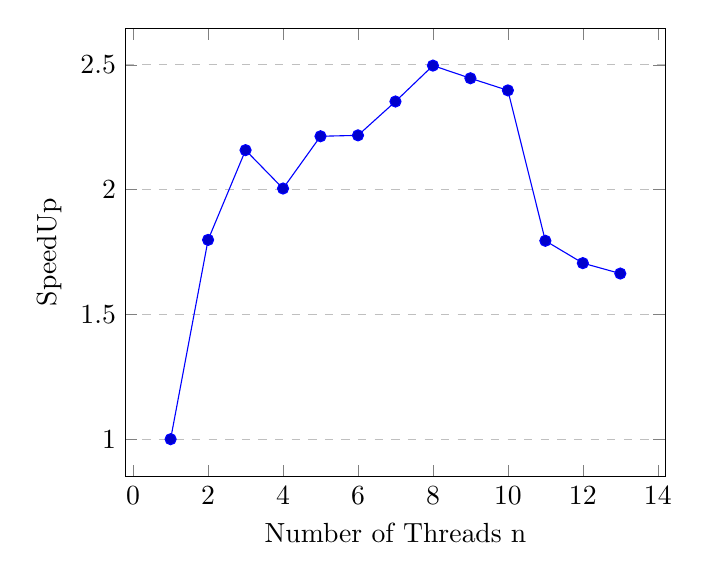
\begin{tikzpicture}
		\begin{axis}[ 
			xlabel=Number of Threads n,
			ylabel=SpeedUp,
			ymajorgrids=true,
			grid style=dashed,
  				]	 
			\addplot coordinates {
(1               , 1           )
(2               , 1.79857121  )
(3               , 2.158198737 )
(4               , 2.004442056 )
(5               , 2.213830008 )
(6               , 2.217449026 )
(7               , 2.353109394 )
(8               , 2.497054623 )
(9               , 2.446263649 )
(10              , 2.397677483 )
(11              , 1.794993945 )
(12              , 1.705459672 )
(13              , 1.6637626   )
				};
		\end{axis}
	\end{tikzpicture}
\end{figure}

\begin{figure}\centering
	\caption{Number of threads vs Efficiency}\label{fig:threadsEfficiency}
	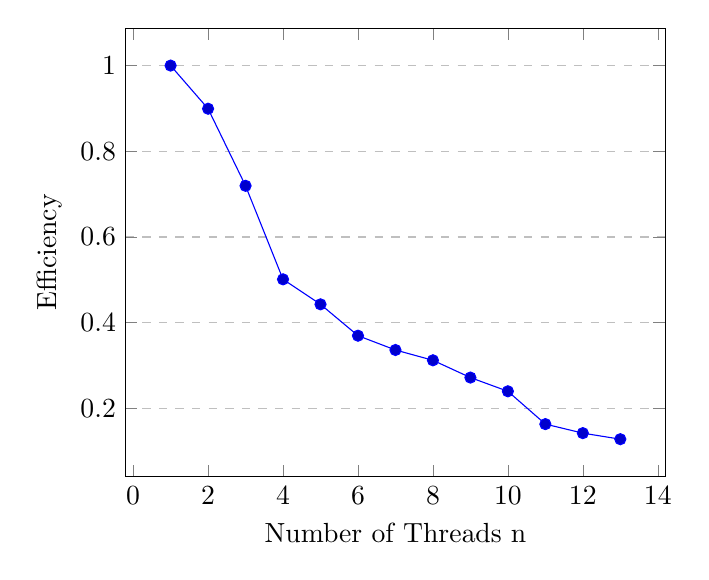
\begin{tikzpicture}
		\begin{axis}[ 
			xlabel=Number of Threads n,
			ylabel=Efficiency,
			ymajorgrids=true,
			grid style=dashed,
  				]	 
			\addplot coordinates {
(1               , 1           )
(2               , 0.899285605  )
(3               , 0.719399579 )
(4               , 0.501110514 )
(5               , 0.442766002 )
(6               , 0.369574838 )
(7               , 0.336158485 )
(8               , 0.312131828 )
(9               , 0.271807072 )
(10              , 0.239767748 )
(11              , 0.163181268  )
(12              , 0.142121639 )
(13              , 0.127981738 )
				};
		\end{axis}
	\end{tikzpicture}
\end{figure}


Now that we presented the collected data, we would like to estimate an approximate time complexity that would fit our \emph{Time Complexity T(n,p)} data. For that we will apply the method described before: \emph{Linear least squares}. After the analysis, we will adopt for our data the following equation for the \emph{Time Complexity T(n,p)}.
\[191.451-54.8072 log(x)\] 
which asymptotically is equivalent on average to 
\[\theta(log(x))\] 
We can verify the details of the \emph{Linear least squares} method in the figure \ref{fig:Experiment_003} or in the following link:	
\\\\
\url{http://www.wolframalpha.com/input/?i=fit+%281+%2C+223.816%29%2C%282+%2C+124.441%29%2C%283+%2C+103.705%29%2C%284+%2C+111.66+%29%2C%285+%2C+101.099%29%2C%286+%2C+100.934%29%2C%287+%2C+95.115+%29%2C%288+%2C+89.632+%29}
\\\\

\begin{figure}\centering
	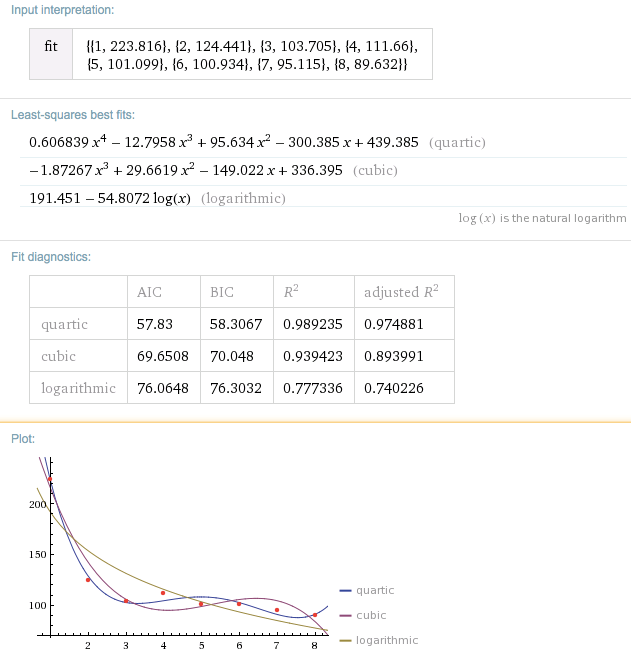
\includegraphics[scale=0.65]{Experiment_003}
	\caption{Least-squares Analysis - Threads}\label{fig:Experiment_003}
\end{figure}

In order to explain our results we will cite one article \cite{SF2008}, Our first problem was to determine the optimal number of threads that would be suitable for our task. What we did was to run the framework with several number of threads (from 1 to 13) in our limited hardware environment, and according to the average of the results of the execution time versus the number of threads (as shown in table \ref{tab:threadsTime} and figure \ref{fig:threadsTime}) and the theory; there is some \emph{threshold} \cite[p. 9]{T2011} where when p increases, the time decreases, but after this \emph{threshold}, the decreasing time is slower and slower with increasing \emph{p}; which means that the efficiency decreases and the cost starts to grow. Each Parallel Algorithm has its own flexibility to choose \emph{n} if \emph{p} changes or to choose \emph{p} if \emph{n} changes. After this, comes the concept of \emph{Time Scallability} (shown on the figure \ref{fig:threadsTime}), which is the minimum p, such that time is asymptotically optimal. If we analyze the figure \ref{fig:threadsTime} or the table \ref{tab:threadsTime} we can observe that after some \emph{threshold}, after adding more and more \emph{threads}, the time became worser; so after this, we will choose the number of threads that will keep a good performance without degrading the Execution time; which in our case will be 8 threads. 

Earlier we mention that we would explain the "why" of our results with such a limited hardware environment (2 cores). An approach of this answer was given in the section \ref{concurrency}; which states that the sequential version of our framework makes the processor \emph{iddle} for a long time (Almost "light years" in processor time :-)), and all this time the processor is waiting for download or I/O operations to finish. And after implementing 8 threads, our \emph{Time T(n,p)} and \emph{Speedup S(n,p)} are maximum in our environment. 

We can conclude that this improvement make an important impact on the performance of the framework \emph{for "free"}; because we are using exactly the same hardware. And the same behavior is expected for bigger \emph{sizes of the problem "n"} in larger \emph{infrastructures}.

\section{Results.}

In order to present the results, we will present the analyzed companies which are shown in the table \ref{tab:analyzedCompanies}, and we will choose one company to analyze it a bit deeper which will be \emph{AAPL - Apple Inc.},  and the reasons why we choose this company are simple: 
\begin{itemize}
	\item Apple now is the most valuable company in History \cite{BE2012} in terms of market capitalization (total value of the issued shares of a publicly traded company; it is equal to the share price times the number of shares outstanding.).
	\item Apple Overtakes Coca-Cola as World’s Most Valuable Brand \cite{AK2013}.
\end{itemize}
Our news crawler obtained 15,067 articles; from those 8,810 (58.47\%) were subject to heuristics in order to extract the article. The rest 6,257 (41.52\%) articles were extracted accurately using locators. From this 15,067 articles 9,567 (63.50\%) were positive and 5,500 (36.50\%) were negative.

\begin{table}\centering
	\caption{Analyzed companies}\label{tab:analyzedCompanies}
   	\begin{tabular}{ | p{3cm\textwidth} | p{7cm\textwidth} |}
   	\hline

\textbf{Symbol}           & \textbf{Name} \\\hline

AAPL   & Apple Inc.                        \\\hline
AXP    & American Express                  \\\hline
BA     & Boeing                            \\\hline
BNS    & The Nova Scotia Bank              \\\hline
CAT    & Caterpillar                       \\\hline
CSCO   & Cisco                             \\\hline
CVX    & Chevron                           \\\hline
DD     & Du Pont                           \\\hline
DIS    & The Walt Disney Company           \\\hline
GE     & General Electric                  \\\hline
GS     & Goldman Sachs Group               \\\hline
HD     & Home Depot                        \\\hline
HMC    & Honda Motor                       \\\hline
IBM    & IBM                               \\\hline
INTC   & Intel                             \\\hline
JNJ    & Johnson \& Johnson                \\\hline
JPM    & JPMorgan Chase                    \\\hline
KO     & Coca Cola                         \\\hline
MCD    & McDonald's                        \\\hline
MMM    & 3M                                \\\hline
MRK    & Merck                             \\\hline
MSFT   & Microsoft                         \\\hline
NKE    & Nike                              \\\hline
OXY    & Occidental Petroleum Corporation  \\\hline
PBR    & Petróleo Brasileiro - Petrobras   \\\hline
PFE    & Pfizer                            \\\hline
PG     & Procter \& Gamble                 \\\hline
T      & AT\&T                             \\\hline
TRV    & Travelers Companies               \\\hline
UNH    & United Health Companies           \\\hline
UTX    & United Technologies Corp          \\\hline
V      & Visa                              \\\hline
VZ     & Verizon Communications            \\\hline
WMT    & Wal-Mart                          \\\hline
XOM    & Exxon Mobil                       \\\hline
YPF    & Yacimientos Petrolíferos Fiscales \\\hline

    \end{tabular}
\end{table}

First of all we will analyze the correlation of the chosen company in the previously mentioned period (\emph{April 1st, 2014 - April 30th, 2014}). But before that, we will give a brief overview about: \emph{Pearson product-moment correlation coefficient} according to wikipedia \cite{PP2014}.
\\
 Pearson product-moment correlation coefficient (Pearson's r) is a measure of the linear correlation (dependence) between two variables X and Y, giving a value between +1 and \−1 inclusive, where 1 is total positive correlation, 0 is no correlation, and \−1 is total negative correlation. It is widely used in the sciences as a measure of the degree of linear dependence between two variables.

Pearson's correlation coefficient between two variables is defined as the covariance of the two variables divided by the product of their standard deviations. The form of the definition involves a "product moment", that is, the mean (the first moment about the origin) of the product of the mean-adjusted random variables; hence the modifier product-moment in the name.

Pearson's correlation coefficient when applied to a sample is commonly represented by the letter r and may be referred to as the sample correlation coefficient or the sample Pearson correlation coefficient. And is calculated as follows: 

\[r = \frac{\sum ^n _{i=1}(X_i - \bar{X})(Y_i - \bar{Y})}{\sqrt{\sum ^n _{i=1}(X_i - \bar{X})^2} \sqrt{\sum ^n _{i=1}(Y_i - \bar{Y})^2}}\] 
\\\\
Now that we have a small background about the \emph{Pearson correlation coefficient} we will proceed to interpret the obtained data. We will start with the table \ref{tab:ResultsApple} which shows the news articles (positive and negative) and the price and delta (variation of the current price according to the price of the day before). And if we apply the \emph{Pearson correlation coefficient} to the \emph{Number of positive articles} and to \emph{Price delta} we would get: \emph{r = -37.83\%} and when we correlate the \emph{Number of negative articles} and the \emph{Price delta} we get \emph{r = -37.85\%}. According to this numbers and to the interpretation of the coefficient; first thing that we can observe is that both numbers have the same direction and they are very close to each other, so this means that in this period if they have good news, their price will somehow drop. And if they have bad news, their price as well will drop, and the negative news will have more impact that positive ones.


\begin{table}\centering
	\caption{Results AAPL}\label{tab:ResultsApple}
   	\begin{tabular}{ | p{2cm\textwidth} | p{2cm\textwidth} | p{2cm\textwidth} | p{2cm\textwidth} | p{2.5cm\textwidth} |}
   	\hline

\textbf{Date}           & \textbf{Positive} & \textbf{Negative} & \textbf{Price}  & \textbf{PriceDelta\$} \\
01/04/14& 14       & 15       & 541.65 & 4.910035584  \\\hline
02/04/14& 38       & 15       & 542.55 & 0.899965664  \\\hline
03/04/14& 31       & 14       & 538.79 & -3.76001067  \\\hline
04/04/14& 34       & 13       & 531.82 & -6.969979738 \\\hline
07/04/14& 34       & 17       & 523.47 & -8.350027011 \\\hline
08/04/14& 22       & 13       & 523.44 & -0.029968249 \\\hline
09/04/14& 22       & 16       & 530.32 & 6.880000456  \\\hline
10/04/14& 22       & 7        & 523.48 & -6.84005142  \\\hline
11/04/14& 9        & 5        & 519.61 & -3.869992927 \\\hline
14/04/14& 17       & 7        & 521.68 & 2.070005373  \\\hline
15/04/14& 15       & 10       & 517.96 & -3.719968002 \\\hline
16/04/14& 10       & 6        & 519.01 & 1.049988371  \\\hline
17/04/14& 13       & 1        & 524.94 & 5.92998471   \\\hline
21/04/14& 12       & 9        & 531.17 & 6.23         \\\hline
22/04/14& 16       & 16       & 531.7  & 0.530029399  \\\hline
23/04/14& 14       & 12       & 524.75 & -6.9499989   \\\hline
24/04/14& 4        & 3        & 567.77 & 43.01998968  \\\hline
25/04/14& 1        & 5        & 571.94 & 4.169980224  \\\hline
28/04/14& 15       & 7        & 594.09 & 22.15005156  \\\hline
29/04/14& 8        & 7        & 592.33 & -1.760007899 \\\hline
30/04/14& 1        & 5        & 590.09 & -2.239987541 \\\hline

    \end{tabular}
\end{table}

In the table \ref{tab:ResultsApple}, we focused in a period of one month. Now we will have a look to the table {tab:ResultsApple}, which presents the correlation coefficient in a weekly basis. And as we can see, the weekly correlations are quiet different between each others and from the table \ref{tab:ResultsApple}, and the negative correlations appear several times in the analysis.

\begin{table}\centering
	\caption{AAPL Weekly correlation}\label{tab:ResultsApple}
   	\begin{tabular}{ | p{1.8cm\textwidth} | p{1cm\textwidth} | p{1cm\textwidth} | p{1.1cm\textwidth} | p{1.1cm\textwidth} | p{2.5cm\textwidth} | p{2.5cm\textwidth} |}
   	\hline

\textbf{Date}           & \textbf{Pos.} & \textbf{Neg.} & \textbf{Price}  & \textbf{Delta (\$)} & \textbf{Pos.-price corr.} & \textbf{Neg-price corr.} \\\hline
01/04/14 & 14   & 15   & 541.65 & 4.91         &                    &                     \\\hline
02/04/14 & 38   & 15   & 542.55 & 0.90         &                    &                     \\\hline
03/04/14 & 31   & 14   & 538.79 & -3.76        &                    &                     \\\hline
04/04/14 & 34   & 13   & 531.82 & -6.97        & -0.645596372       & 0.935331709         \\\hline
07/04/14 & 34   & 17   & 523.47 & -8.35        &                    &                     \\\hline
08/04/14 & 22   & 13   & 523.44 & -0.03        &                    &                     \\\hline
09/04/14 & 22   & 16   & 530.32 & 6.88         &                    &                     \\\hline
10/04/14 & 22   & 7    & 523.48 & -6.84        &                    &                     \\\hline
11/04/14 & 9    & 5    & 519.61 & -3.87        & -0.242402973       & 0.321685525         \\\hline
14/04/14 & 17   & 7    & 521.68 & 2.07         &                    &                     \\\hline
15/04/14 & 15   & 10   & 517.96 & -3.72        &                    &                     \\\hline
16/04/14 & 10   & 6    & 519.01 & 1.05         &                    &                     \\\hline
17/04/14 & 13   & 1    & 524.94 & 5.93         & -0.177342173       & -0.95274704         \\\hline
21/04/14 & 12   & 9    & 531.17 & 6.23         &                    &                     \\\hline
22/04/14 & 16   & 16   & 531.7  & 0.53         &                    &                     \\\hline
23/04/14 & 14   & 12   & 524.75 & -6.95        &                    &                     \\\hline
24/04/14 & 4    & 3    & 567.77 & 43.02        &                    &                     \\\hline
25/04/14 & 1    & 5    & 571.94 & 4.17         & -0.549262067       & -0.715444882        \\\hline
28/04/14 & 15   & 7    & 594.09 & 22.15        &                    &                     \\\hline
29/04/14 & 8    & 7    & 592.33 & -1.76        &                    &                     \\\hline
30/04/14 & 1    & 5    & 590.09 & -2.24        & 0.874501955        & 0.514829914    \\\hline    

    \end{tabular}
\end{table}

Finally we present the correlations between positive and negative articles with the delta price. We can observe in the table \ref{tab:GeneralResults} that the same pattern that we had in the correlation of the data of the table {tab:ResultsApple} repeats here. Not in every case, but usually both numbers are somehow close to each other and that news articles are not the only factor that affects the changes in the price of a stock.

\begin{table}\centering
	\caption{Results of the correlations for each analyzed company}\label{tab:GeneralResults}
   	\begin{tabular}{ | p{2cm\textwidth} | p{3.5cm\textwidth} | p{3.5cm\textwidth} | p{3.5cm\textwidth} | }
   	\hline
\textbf{Company} & \textbf{Positve-Delta Price} & \textbf{Negative-Delta Price} & \textbf{Difference (abs)}  \\\hline
AAPL    & -37.83\%           & -37.85\%            & -0.02\%  \\\hline
AXP     & -42.30\%           & -41.30\%            & 1.00\%   \\\hline
BA      & -37.82\%           & -30.10\%            & 7.72\%   \\\hline
BNS     & -6.64\%            & -14.41\%            & -7.77\%  \\\hline
CAT     & 14.64\%            & 29.17\%             & -14.52\% \\\hline
CAT     & -16.68\%           & -24.23\%            & -7.55\%  \\\hline
CVX     & -21.48\%           & -20.04\%            & 1.43\%   \\\hline
DD      & -20.96\%           & -32.00\%            & -11.04\% \\\hline
DIS     & -21.40\%           & -28.47\%            & -7.08\%  \\\hline
GE      & -44.37\%           & -38.52\%            & 5.85\%   \\\hline
GS      & -71.09\%           & -88.32\%            & -17.23\% \\\hline
HD      & -32.88\%           & -23.42\%            & 9.46\%   \\\hline
HMC     & -11.01\%           & -8.32\%             & 2.69\%   \\\hline
IBM     & 4.53\%             & 18.44\%             & -13.91\% \\\hline
IBM     & 10.52\%            & -4.29\%             & 6.23\%   \\\hline
JNJ     & -10.87\%           & -9.28\%             & 1.60\%   \\\hline
JPM     & -40.92\%           & -66.41\%            & -25.49\% \\\hline
KO      & -4.39\%            & 13.24\%             & -8.84\%  \\\hline
MCD     & -16.50\%           & -23.79\%            & -7.29\%  \\\hline
MMM     & -6.10\%            & -3.51\%             & 2.59\%   \\\hline
MRK     & -41.52\%           & 0.49\%              & 41.03\%  \\\hline
MSFT    & -12.49\%           & -9.19\%             & 3.30\%   \\\hline
NKE     & 12.13\%            & 23.71\%             & -11.57\% \\\hline
OXY     & -5.87\%            & -2.57\%             & 3.30\%   \\\hline
PFE     & -23.42\%           & -23.69\%            & -0.27\%  \\\hline
PG      & 0.47\%             & 15.96\%             & -15.49\% \\\hline
T       & -3.97\%            & -19.42\%            & -15.45\% \\\hline
TRV     & -5.67\%            & -2.87\%             & 2.80\%   \\\hline
UNH     & -25.98\%           & -40.06\%            & -14.08\% \\\hline
UTX     & -35.10\%           & -48.49\%            & -13.38\% \\\hline
V       & -5.73\%            & -25.02\%            & -19.29\% \\\hline
VZ      & -0.43\%            & -6.19\%             & -5.75\%  \\\hline
WMT     & 3.37\%             & -30.49\%            & -27.13\% \\\hline
XOM     & -38.55\%           & -29.69\%            & 8.86\%   \\\hline
YPF     & 26.45\%            & 18.48\%             & 7.97\%  \\\hline

    \end{tabular}
\end{table}




	\setsecnumdepth{part}

	\begin{conclusion}
		\section{Conclusions}

As we proposed since the beginning, there are several factors that affects the price of a particular stock, besides the most common one: \emph{supply and demmand}, our initial position and the most natural was that the positive news are positively correlated with the positive increments of the stock and vice-versa, the negative news are positively correlated with the drops in the stock prices. 

At the beginning what we tried to achieve was some numerical correlation by accounting qualitative factors, here came to play the news articles. This articles could have positive or negative polarity and somehow, according to our initial position and to the data obtained we can say that in most of cases the companies has almost same correlation in positive and negative articles, usually negative, which states that only by publishing news for a company that follows this pattern, means that the stock price may not improve, indeed it will go down.

Most of the work that we are doing here is about to structure information that doesn't have a particular, uniform or homogeneous structure. So, according to the processed information, it is shown once again that this is a particularly difficult and time consuming task to automatize the retrieval of unstructured information. In our case this happen because every Web page has different structure; even though they could have a strict HTML structure, but we are not talking about it, but to the location of the information we want to retrieve from  the different sources of information.

Web 2.0 plays an important role in this work; because it allows users to interact and collaborate as creators of content. In our case, this work was possible to developed because by these days we have the appropriate tools and the availability of the data to do a research like this. In our case the content creators are every reporter that works for a News Portal writing articles.

It's Strongly Recommended for Web Crawlers to implement \emph{Parallelism}. Because the CPU while is waiting for downloading a Web Page or performing I/O operations, is wasting a lot of CPU cycles that could be used by another thread in order to do some useful computation.

\section{Future work}

Here we will mention some directives regarding this work. In previous work that have been done in this topic, one limitation was the number of articles; in our case as mentioned in the results section we retrieve more than 15,000 articles for the 36 companies in one month. So it would be worth to get one more level of detail by trying to get the published time of the articles and perform a real-time analysis with the stock prices.

Besides, we can apply more advanced statistical methods in order to analyze the causality of the events. For this we recommend the ARMA Models which stands for autoregressive–moving-average (ARMA) models.

As we know, heuristics are basically experienced-based techniques for problem solving. In our case we applied heuristics to try to extract a news article from a host that we haven't construct it's locator; to this heuristic technique in our work we called it \emph{Generic Locator}, and the future work is to try to improve this algorithm in order to increase the rate of extracted news articles.

Finally, the last directive would be to consider the implementation of the Web 3.0 (Semantic Web) in the articles we retrieve. In order not only to classify the polarity of the article but to relate the information contained in the article with the web of data.
	\end{conclusion}

	\bibliographystyle{plain}
		\bibliography{ref}

	\printindex
	
	\setsecnumdepth{all}
	\appendix

	\chapter{Glossary}

		\begin{description}
  \item[Algorithm:] step-by-step set of operations to be performed.
  \item[Crawler:] programmable machine / piece of software that receives input, stores and manipulates data, and provides output in a useful format.
  \item[Data structure:] Is a particular way of storing and organising data in a computer so that it can be used efficiently.
  \item[DOM:] The XML DOM defines a standard way for accessing and manipulating XML documents. The DOM presents an XML document as a tree-structure. 
  \item[Dow Jones:] Is a stock market index.
  \item[Framework:] Universal and reusable software environment that provides particular functionality as part of a larger software platform to facilitate development of software applications, products and solutions.
  \item[GATE:] A computer architecture for a broad range of Natural Language Processing tasks, available under the GNU Public License.
  \item[Hash tables:] Data structure used to implement an associative array, a structure that can map keys to values.
  \item[HTML:] HyperText Markup Language is the standard markup language used to create Web pages.
  \item[Http:] Hypertext Transfer Protocol (HTTP) is an application protocol for distributed, collaborative, hypermedia information systems. Is the foundation of the World Wide Web.
  \item[JSOUP:] Java library for working with real-world HTML. It provides a very convenient API for extracting and manipulating data, using the best of DOM, CSS, and jquery-like methods Web page: http://jsouporg/
  \item[Lexemes:] Unit of lexical meaning that exists regardless of the number of inflectional endings it may have or the number of words it may contain.
  \item[Lexicon:] Language's inventory of lexemes.
  \item[News endpoint:] Entry point where news articles are published from several authors.
  \item[NYSE:] New York Stock Exchange
  \item[Query string:] Part of a uniform resource locator that contains data to be passed by web applications.
  \item[RSS:] Family of standard web feed formats to publish frequently updated information: blog entries, news headlines, audio, video.
  \item[S&P 500:] American stock market index based on the market capitalisation of 500 large companies having common stock listed on the NYSE or NASDAQ
  \item[Sentiment analysis:] Use of natural language processing, text analysis and computational linguistics to identify and extract subjective information in source materials
  \item[Stemming:] The process for reducing inflected (or derived) words to their word stem
  \item[Stock market index:] Measurement of the value of a section of the stock market It is computed from the prices of selected stocks It is a tool used by investors and financial managers to describe the market, and to compare the return on specific investments
  \item[Text mining:] Process of deriving high-quality/structured information from text/unstructured information
  \item[Tokenization:] Process of breaking a stream of text up into words, phrases, symbols, or other meaningful elements called tokens
  \item[Web API:] Acronym of "Web Application programming interface", which is defined as a request/response message system, which is exposed on the web.
  \item[WHATWG:] Web Hypertext Application Technology Working Group (WHATWG) is a community of people interested in evolving HTML and related technologies.
\end{description}


	\begin{appendices}
		\chapter{Contents of the CD}\label{app:CDcontent}
			The structure of the content of the CD is presented here.

\begin{figure}
	\dirtree{%
		.1 readme.txt\DTcomment{File with CD contents description}.
		.1 Framework\DTcomment{Directory with Framework implementation}.
		.2 DataBase\DTcomment{Database script}.
		.2 Executable\DTcomment{Executable Jar file}.
		.2 SourceCode\DTcomment{The source code of the framework}.
		.1 Thesis\DTcomment{the directory of \LaTeX{} source codes of the thesis}.
		.2 thesis.pdf\DTcomment{the Diploma thesis in PDF format}.
		.2 Sources\DTcomment{the \LaTeX{} source code files of the thesis}.
		.3 imgs\DTcomment{the thesis figures directory}.
		.3 *.tex\DTcomment{the \LaTeX{} source code files of the thesis}.
	}
\end{figure}
	\end{appendices}
	
\end{document}
